\chapter{Supplementary figures}
\label{sec:plotsetc}
\vspace{-0.75cm}

\begin{figure}
    \centering
    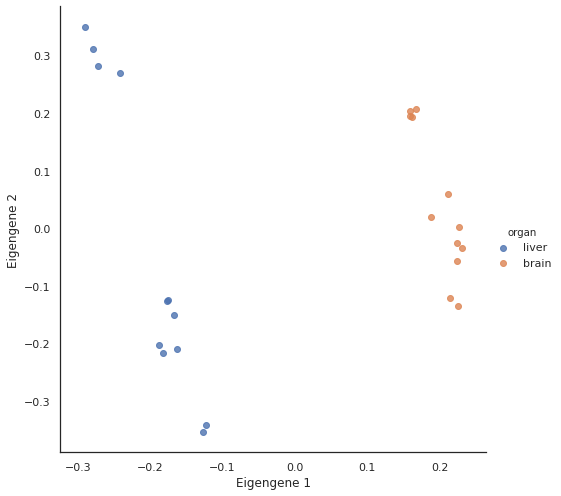
\includegraphics[width=7cm, height=7cm]{Figures&amp;Cover/SampleBehaviourorgan.png}
    \caption{\textbf{Sample behaviour of the preprocessed mRNA expression data.} The mRNA expression data from \textit{M. musculus} liver and brain, that had been \ac{RPM} normalized and log2-transformed, was decomposed using singular value decomposition and the first and second eigengenes were plotted against each other. The samples were coloured by the organ they were sampled from, blue for liver samples and orange for brain samples.}
    \label{fig:SampleBehaviour}
\end{figure}

\begin{figure}
    \centering
    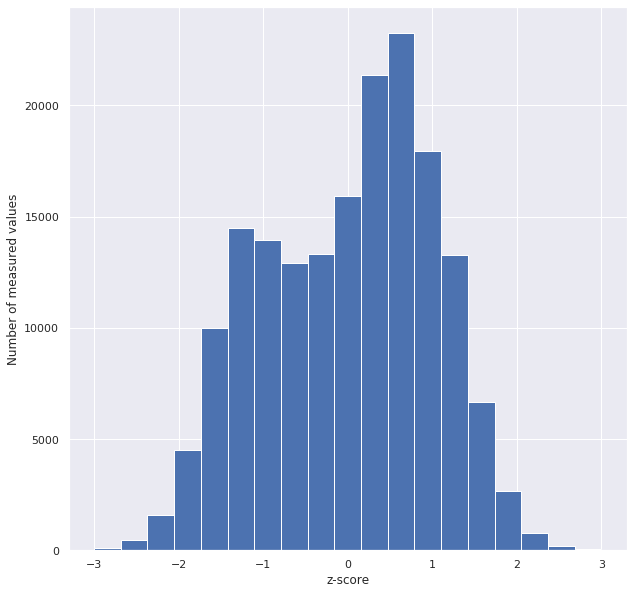
\includegraphics[width=6cm, height=6cm]{Figures&amp;Cover/logdatadistLiver.png}
    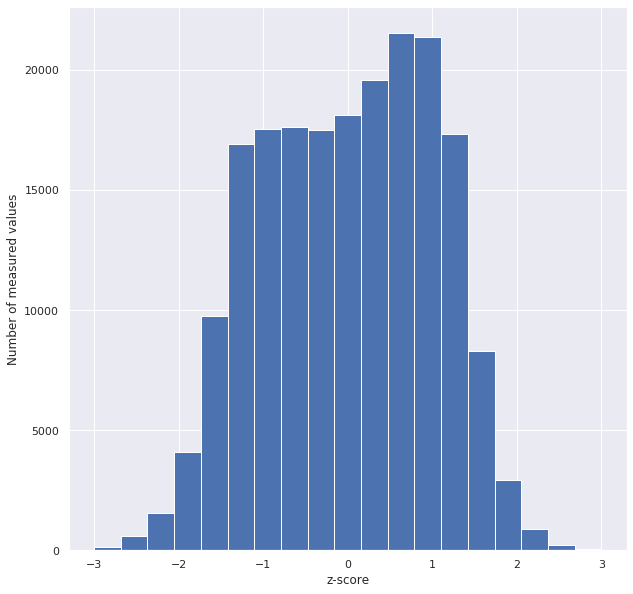
\includegraphics[width=6cm, height=6cm]{Figures&amp;Cover/logdatadistBrain.png}
    \caption{\textbf{Distribution of z-scores for the preprocessed mRNA expression data from \textit{M. musculus} liver (left) and brain (right)}. The z-scores for the mRNA expression values from liver and brain that had been \ac{RPM} normalized and log2-transformed was for each gene calculated and the results were gathered and plotted as a histogram to confirm that they were normally distributed.}
    \label{fig:logdatadist}
\end{figure}

\begin{figure}
    \centering
    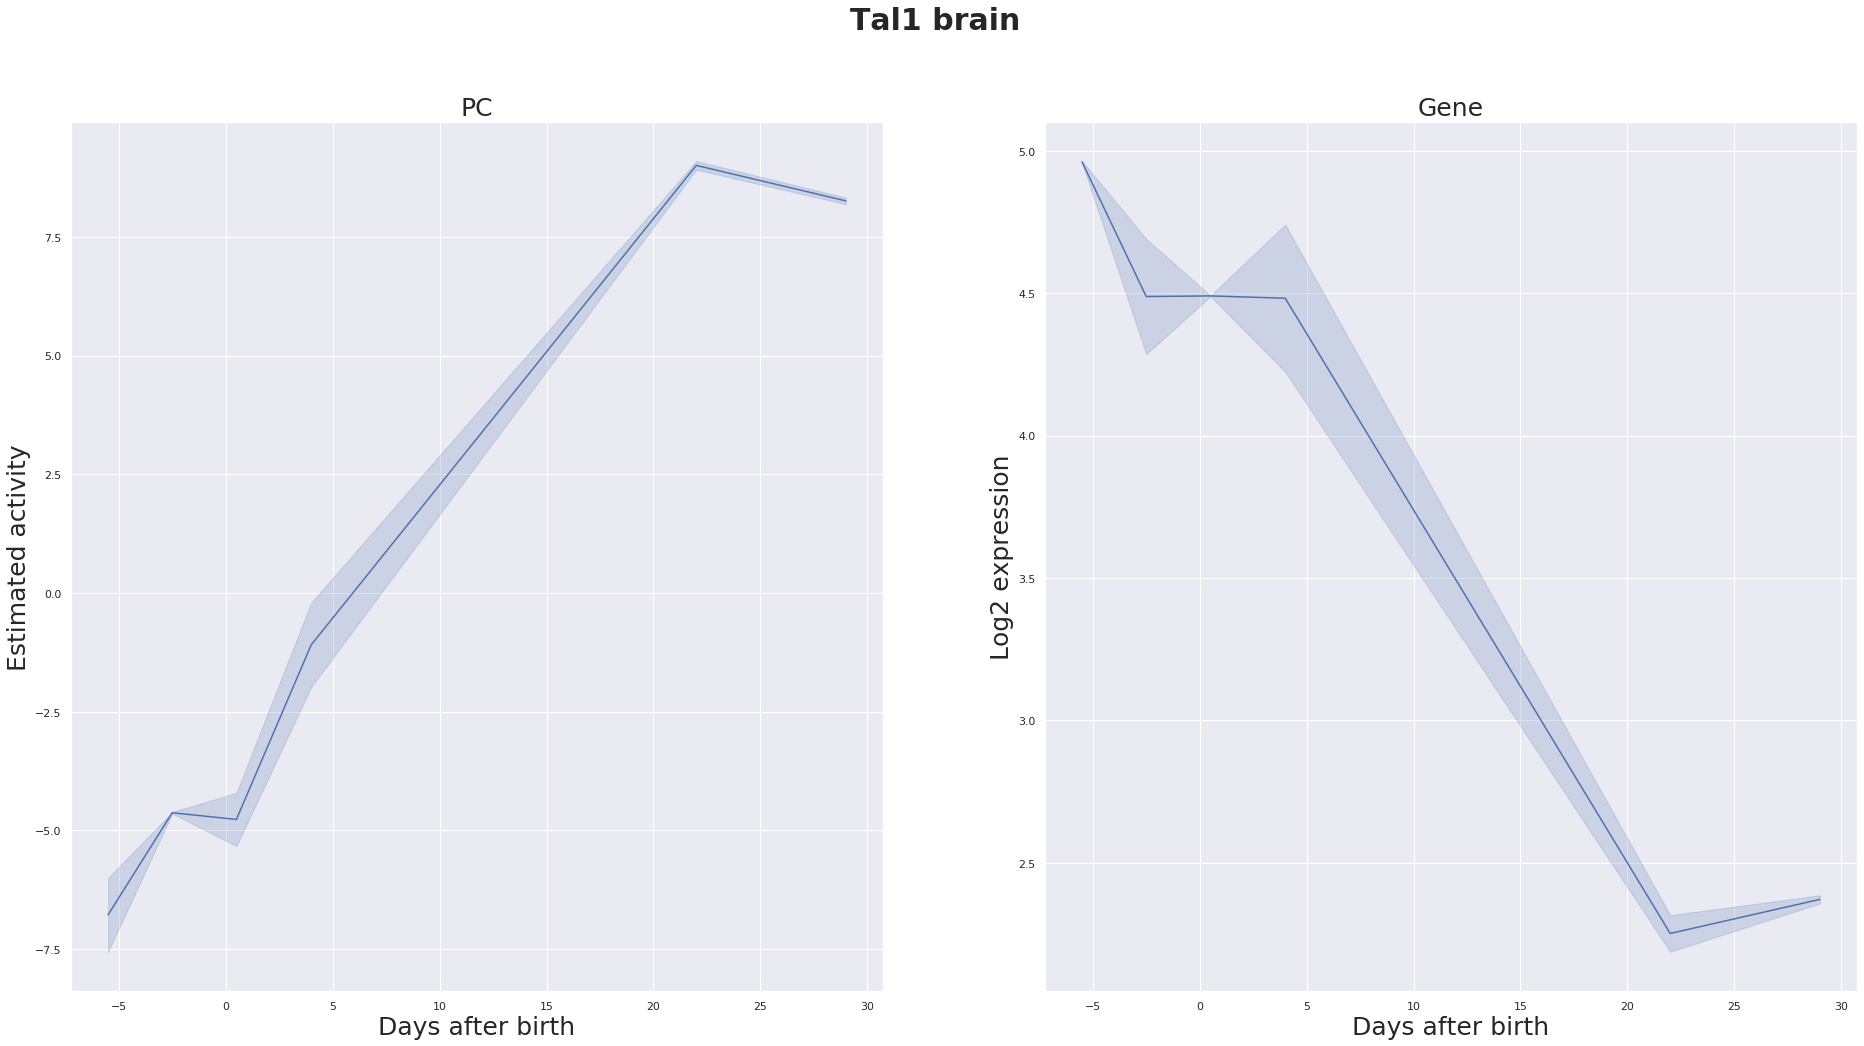
\includegraphics[width=6cm,height=3cm]{Figures&amp;Cover/Activity_Tal1_brain_NonePCremoved_filtering_False.png}
    \hspace{0.25cm}
    \vspace{0.25cm}
    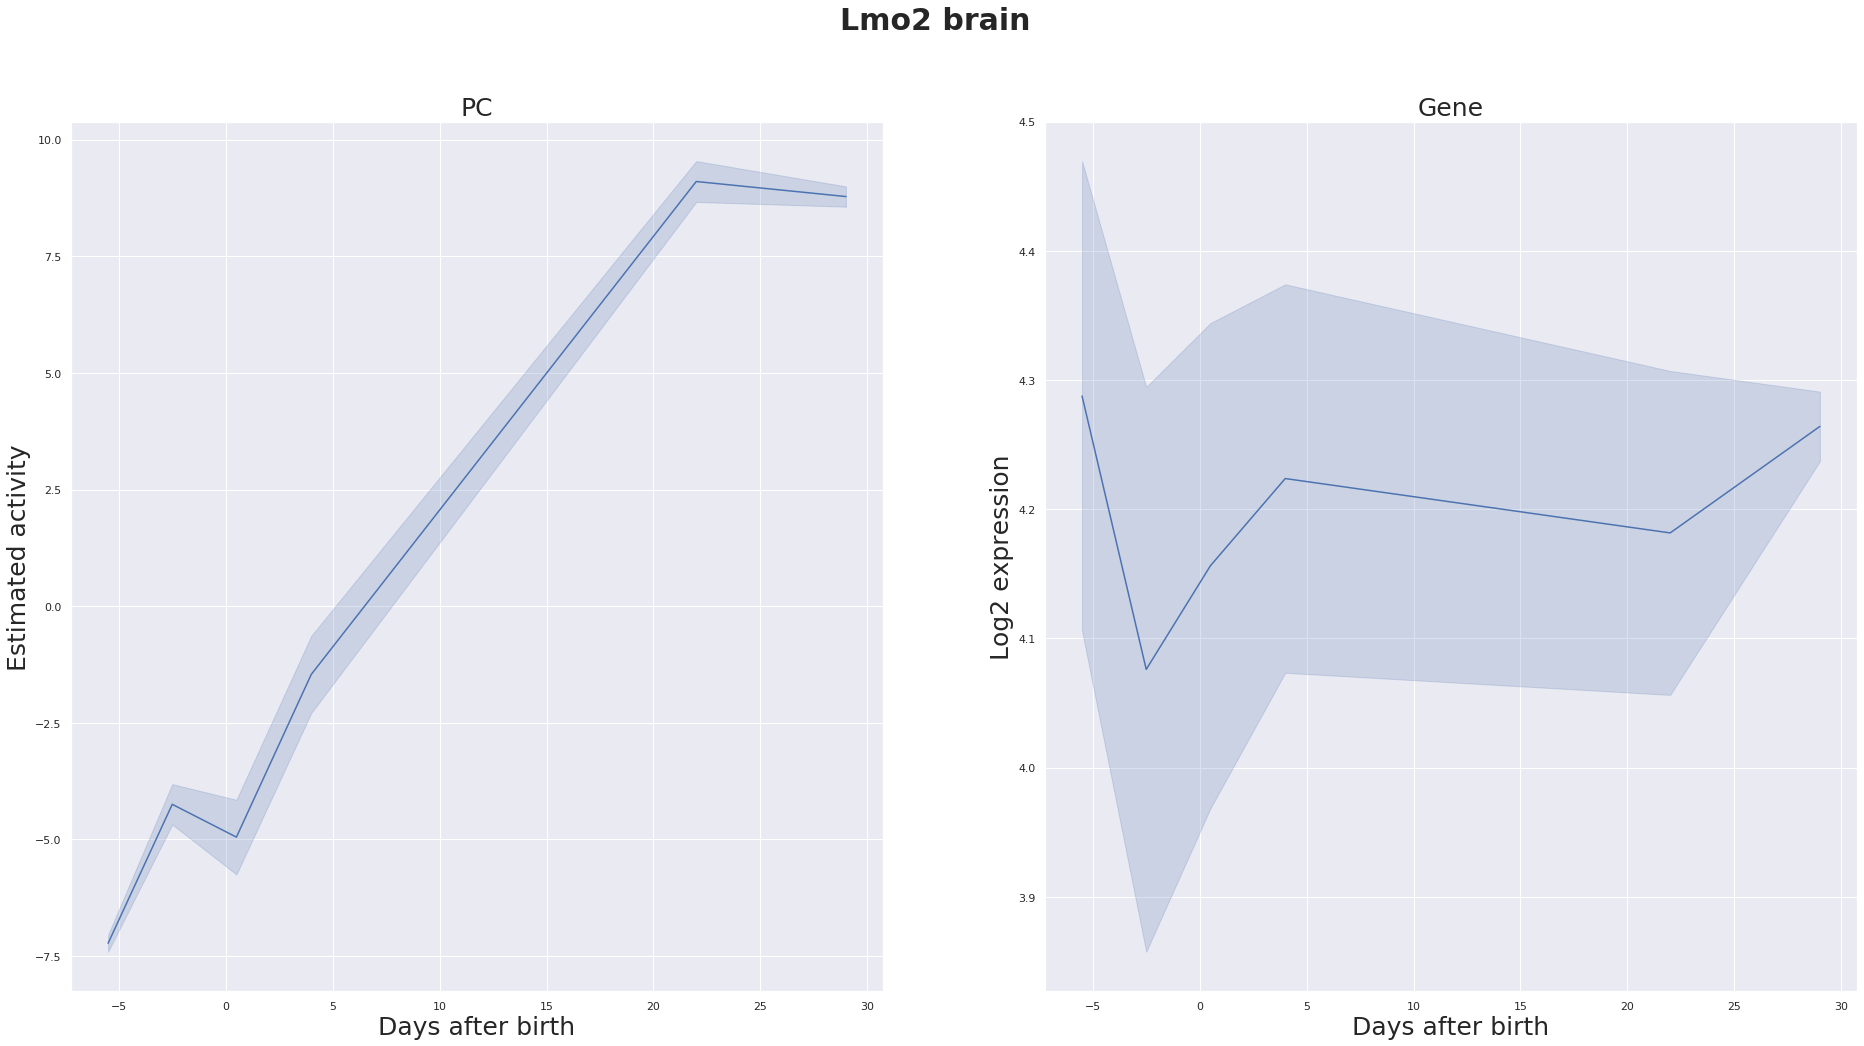
\includegraphics[width=6cm,height=3cm]{Figures&amp;Cover/Activity_Lmo2_brain_NonePCremoved_filtering_False.png}
    \vspace{0.25cm}
    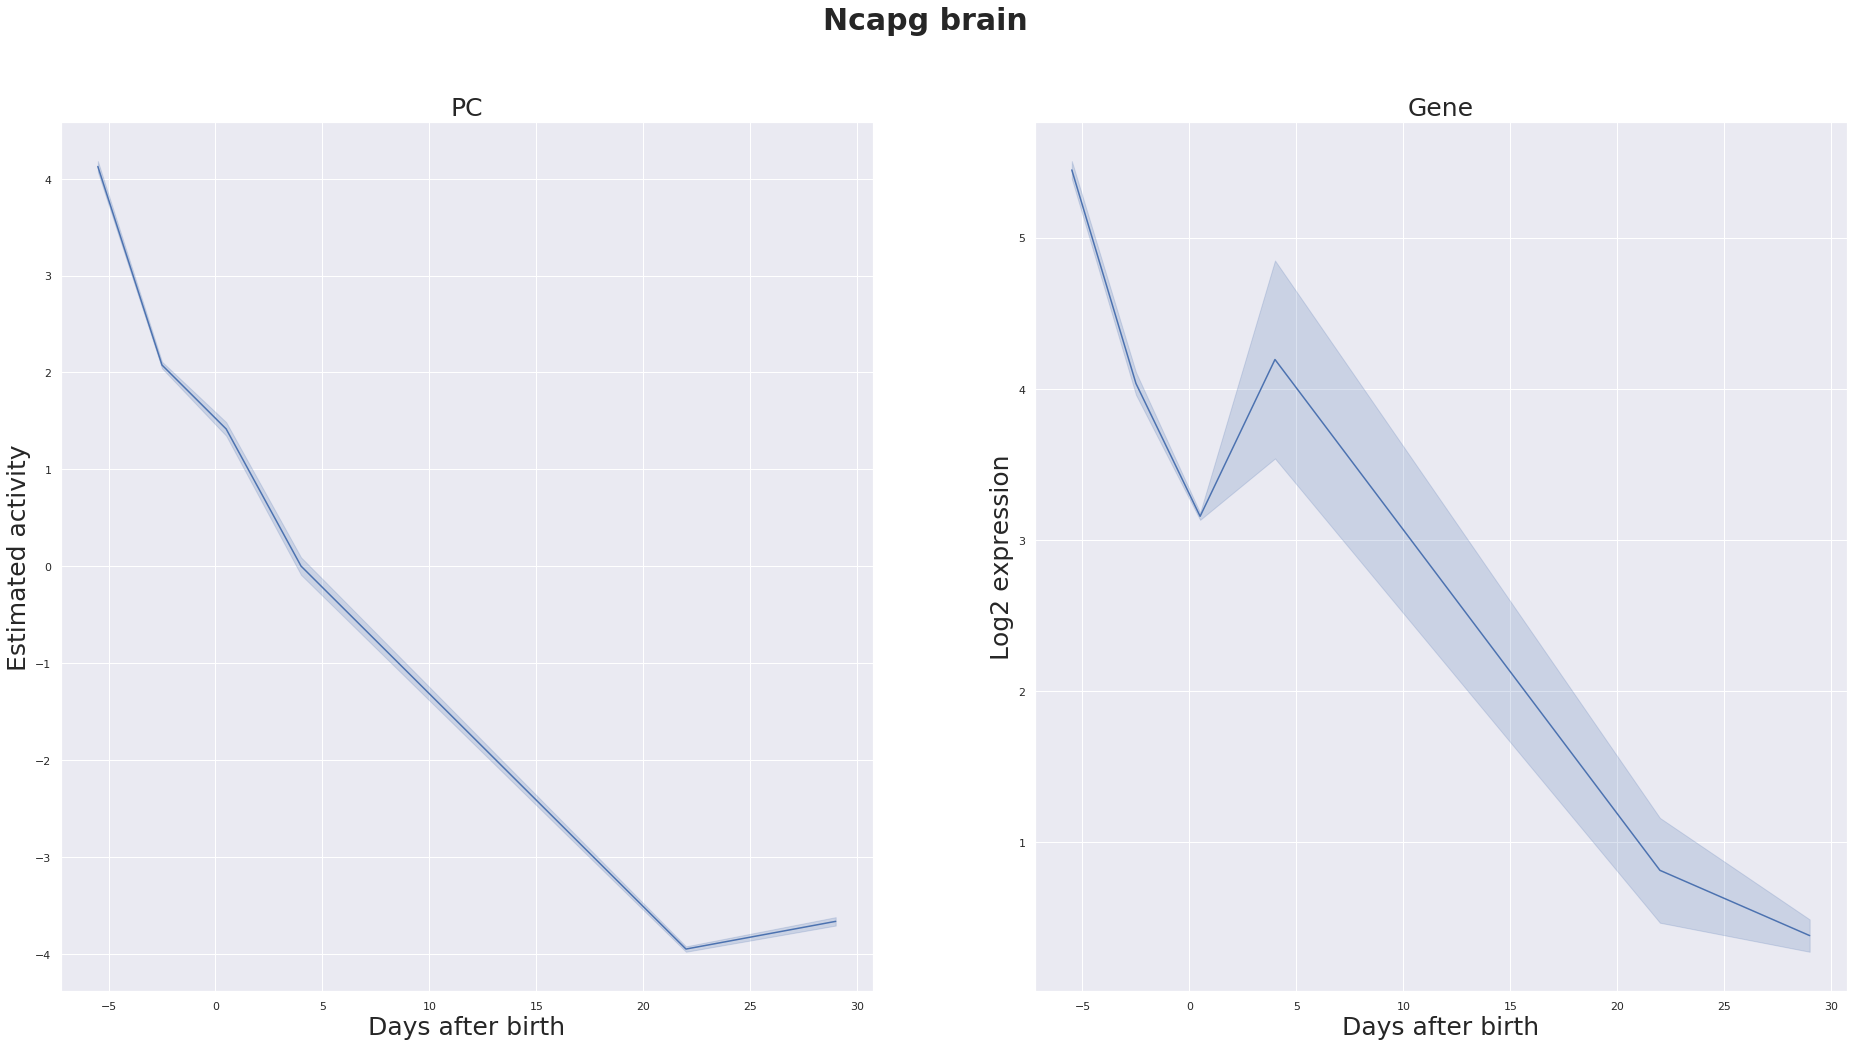
\includegraphics[width=6cm,height=3cm]{Figures&amp;Cover/Activity_Ncapg_brain_NonePCremoved_filtering_False.png}
    \hspace{0.25cm}
    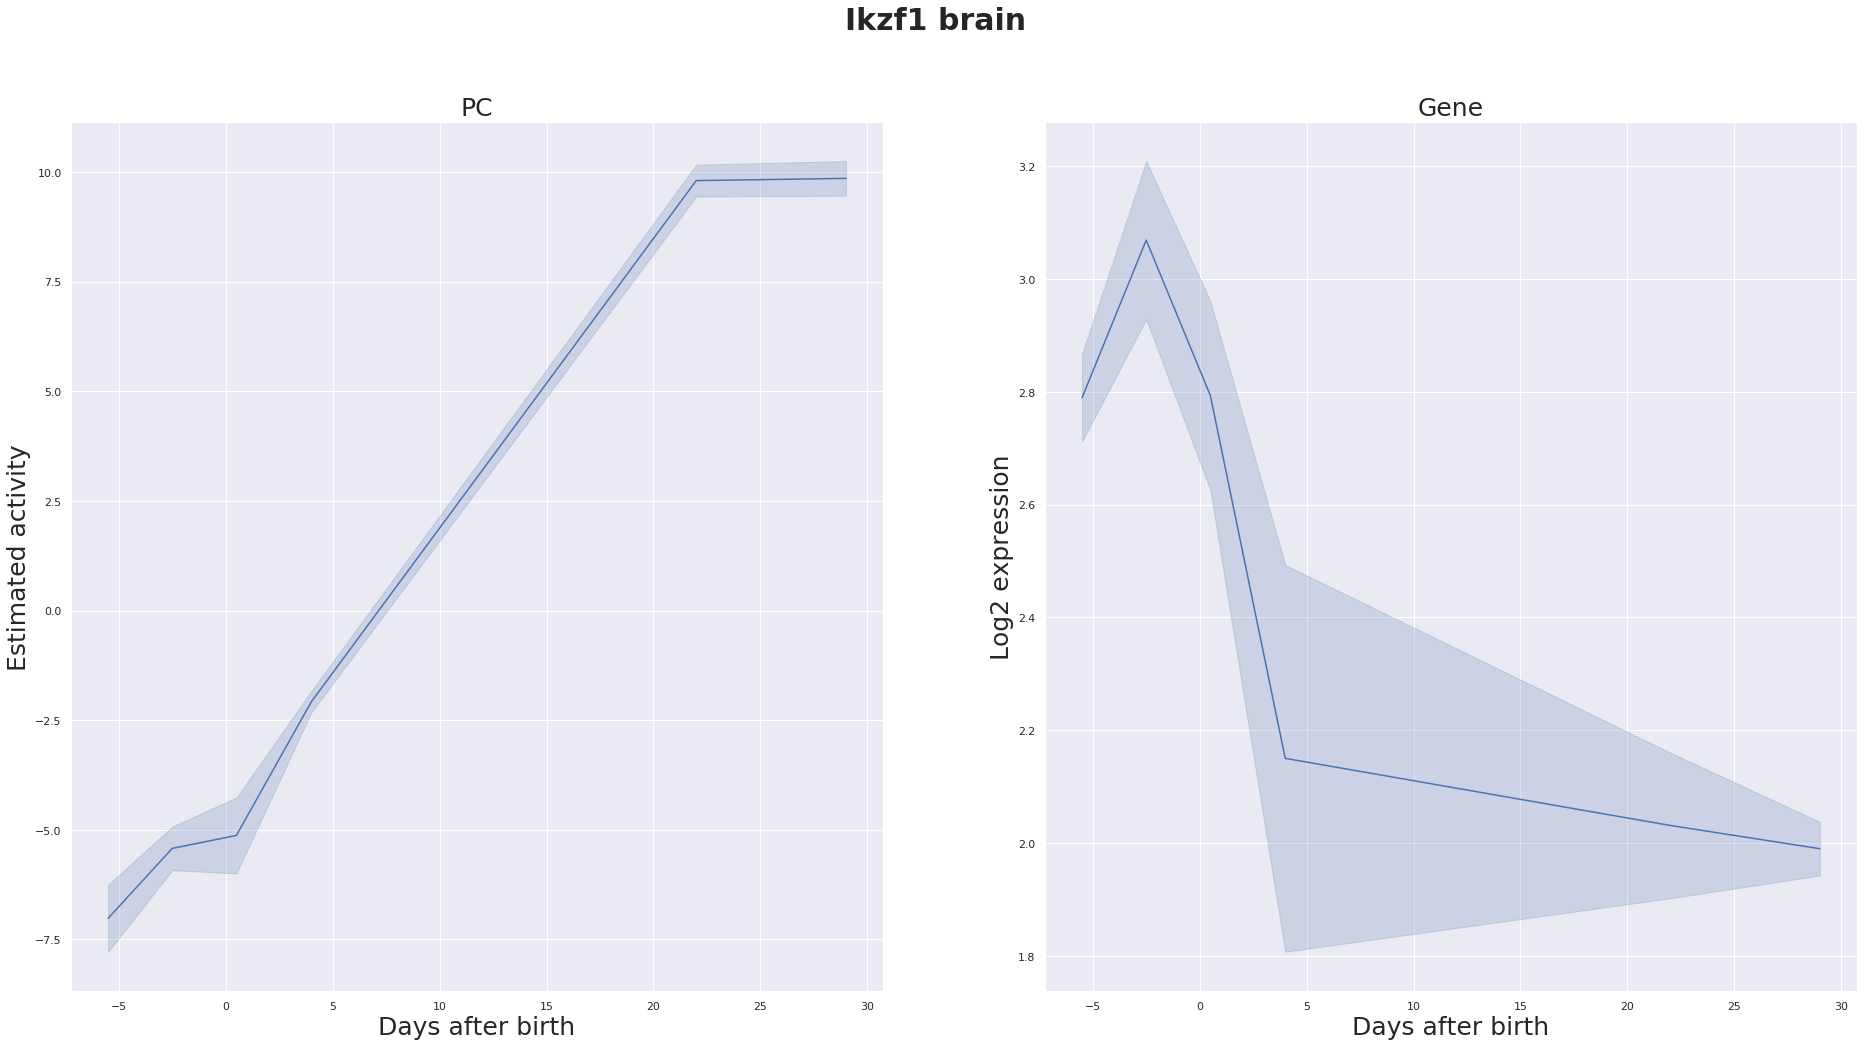
\includegraphics[width=6cm,height=3cm]{Figures&amp;Cover/Activity_Ikzf1_brain_NonePCremoved_filtering_False.png}
    \vspace{0.25cm}
    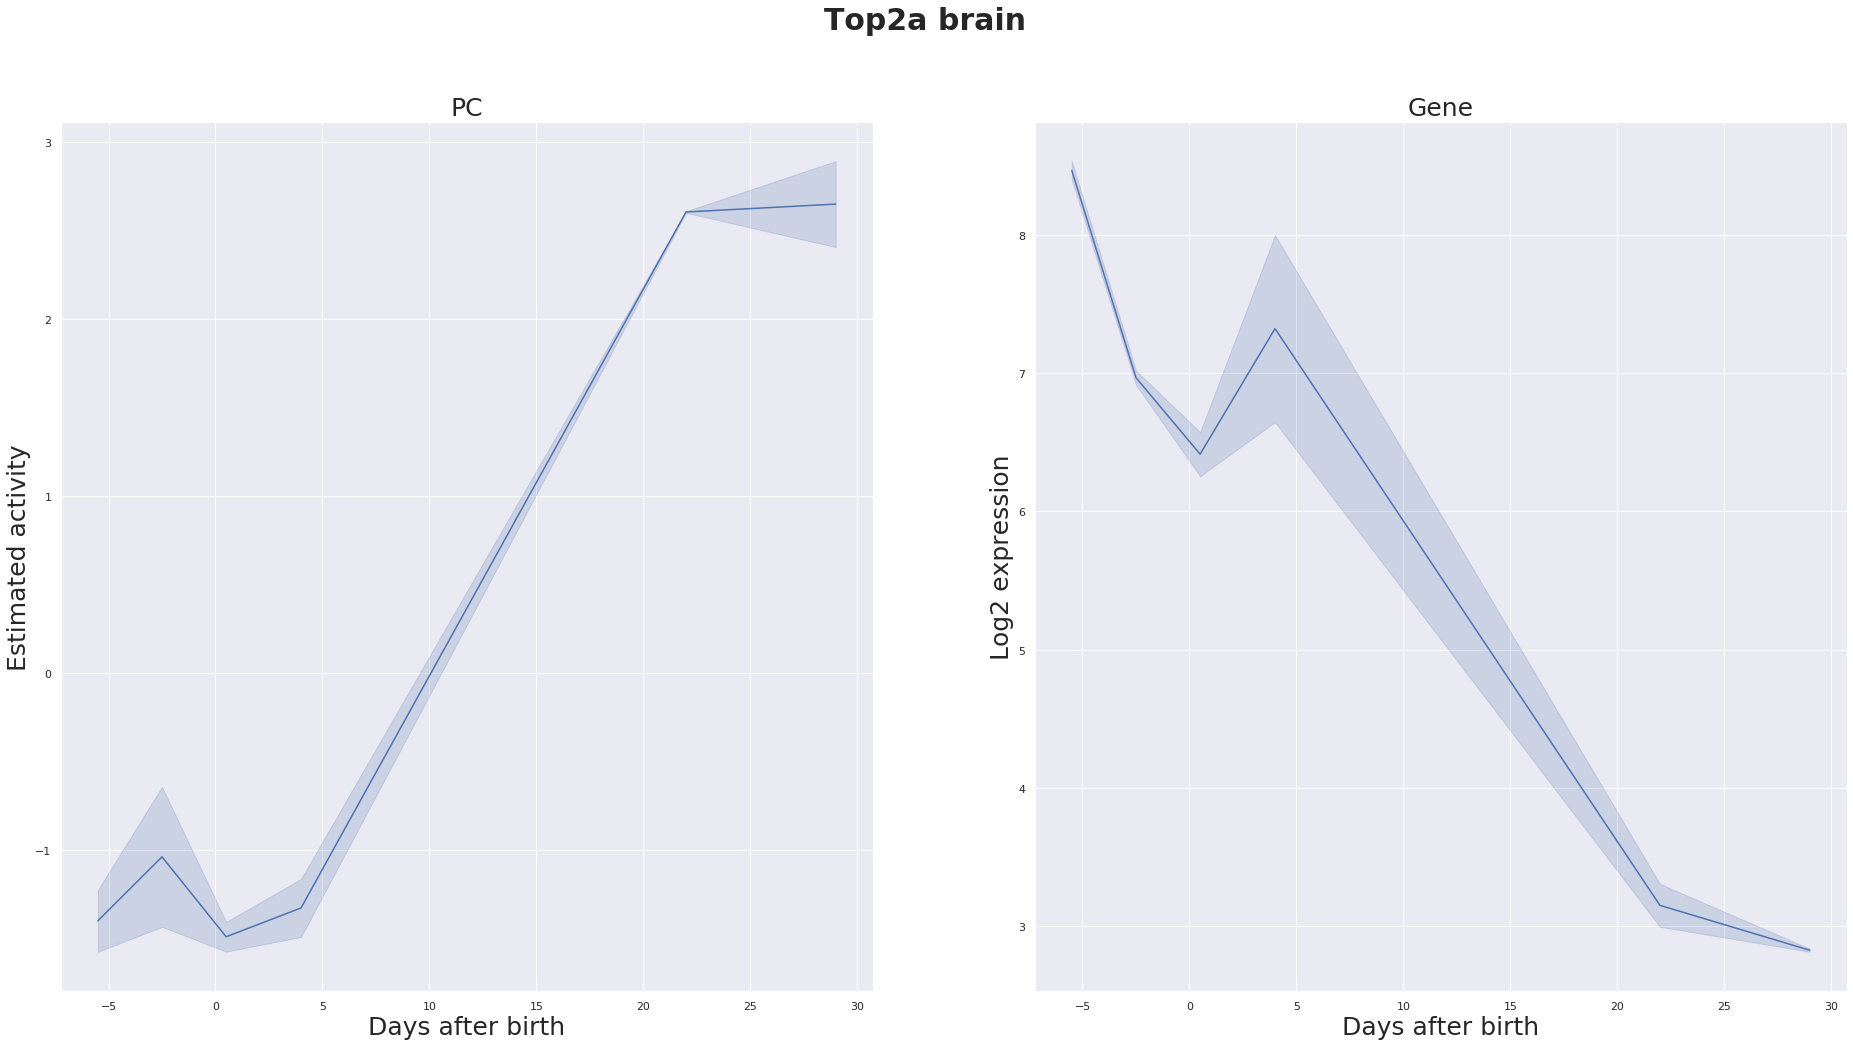
\includegraphics[width=6cm,height=3cm]{Figures&amp;Cover/Activity_Top2a_brain_NonePCremoved_filtering_False.png}
    \hspace{0.25cm}
    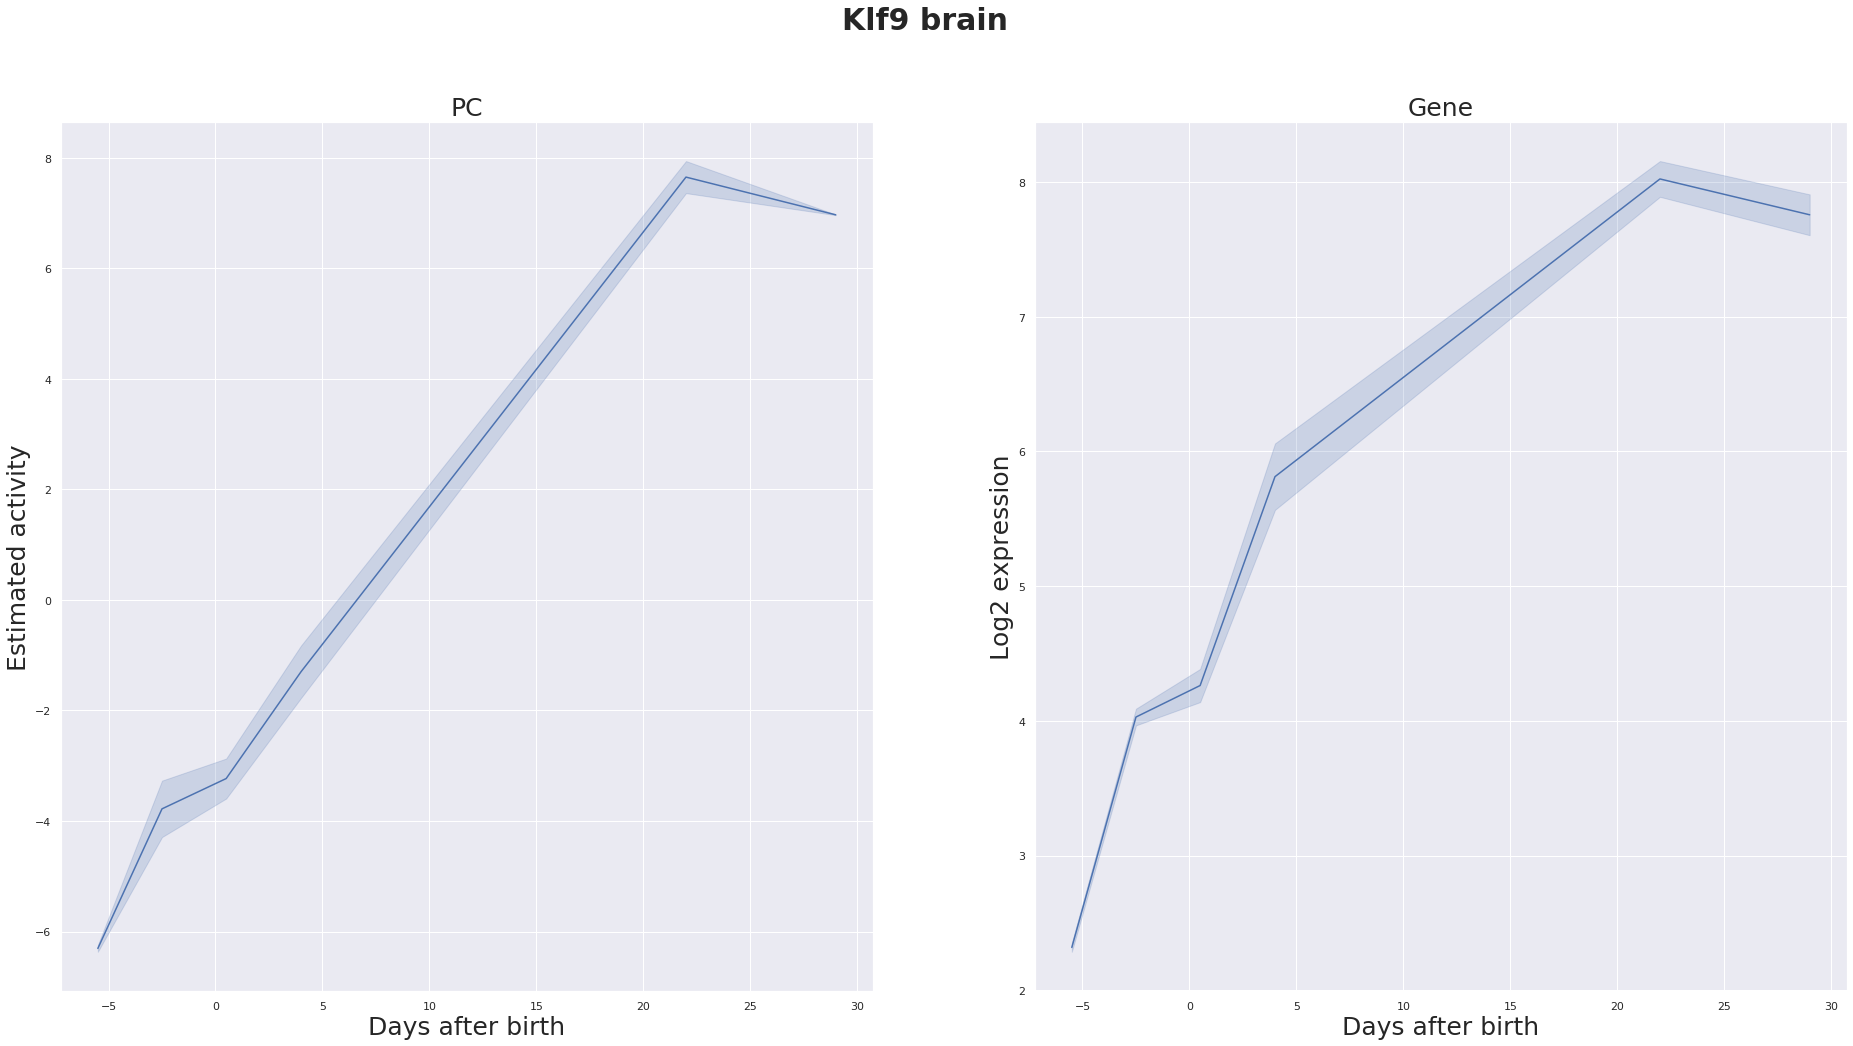
\includegraphics[width=6cm,height=3cm]{Figures&amp;Cover/Activity_Klf9_brain_NonePCremoved_filtering_False.png}
    \vspace{0.25cm}
    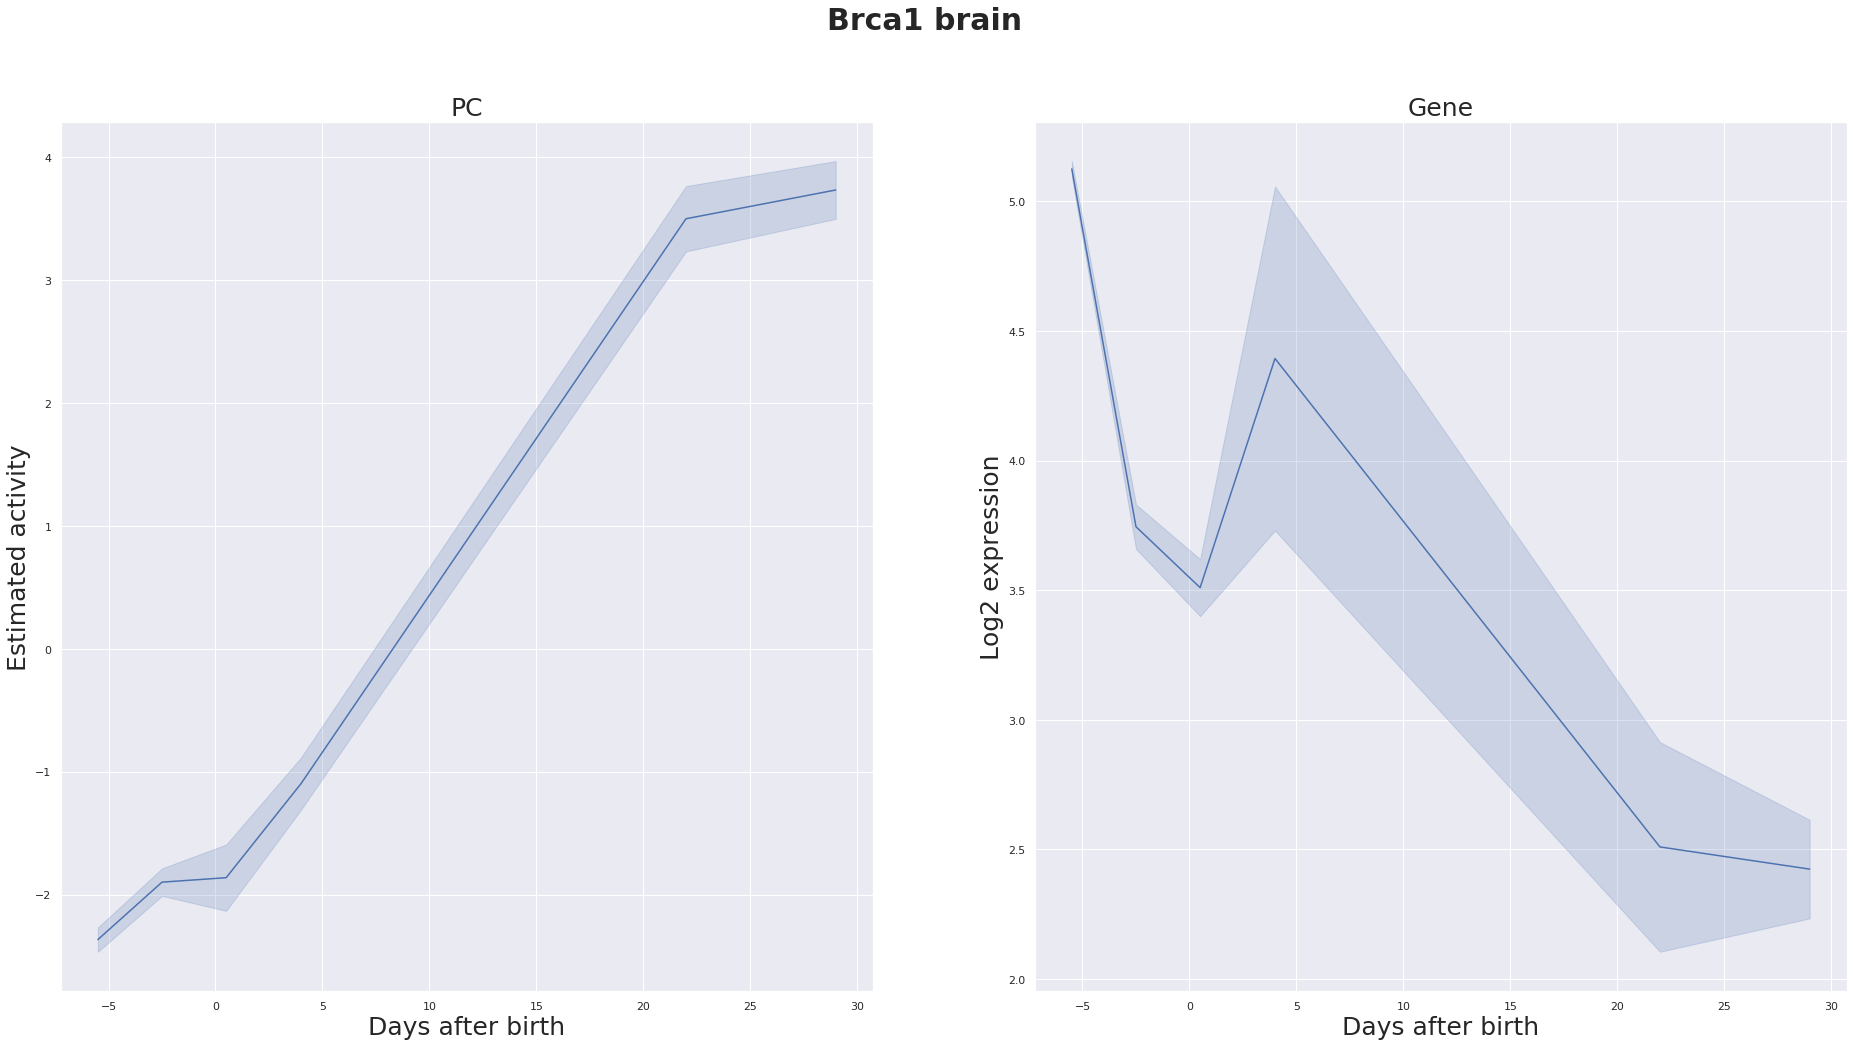
\includegraphics[width=6cm,height=3cm]{Figures&amp;Cover/Activity_Brca1_brain_NonePCremoved_filtering_False.png}
    \hspace{0.25cm}
    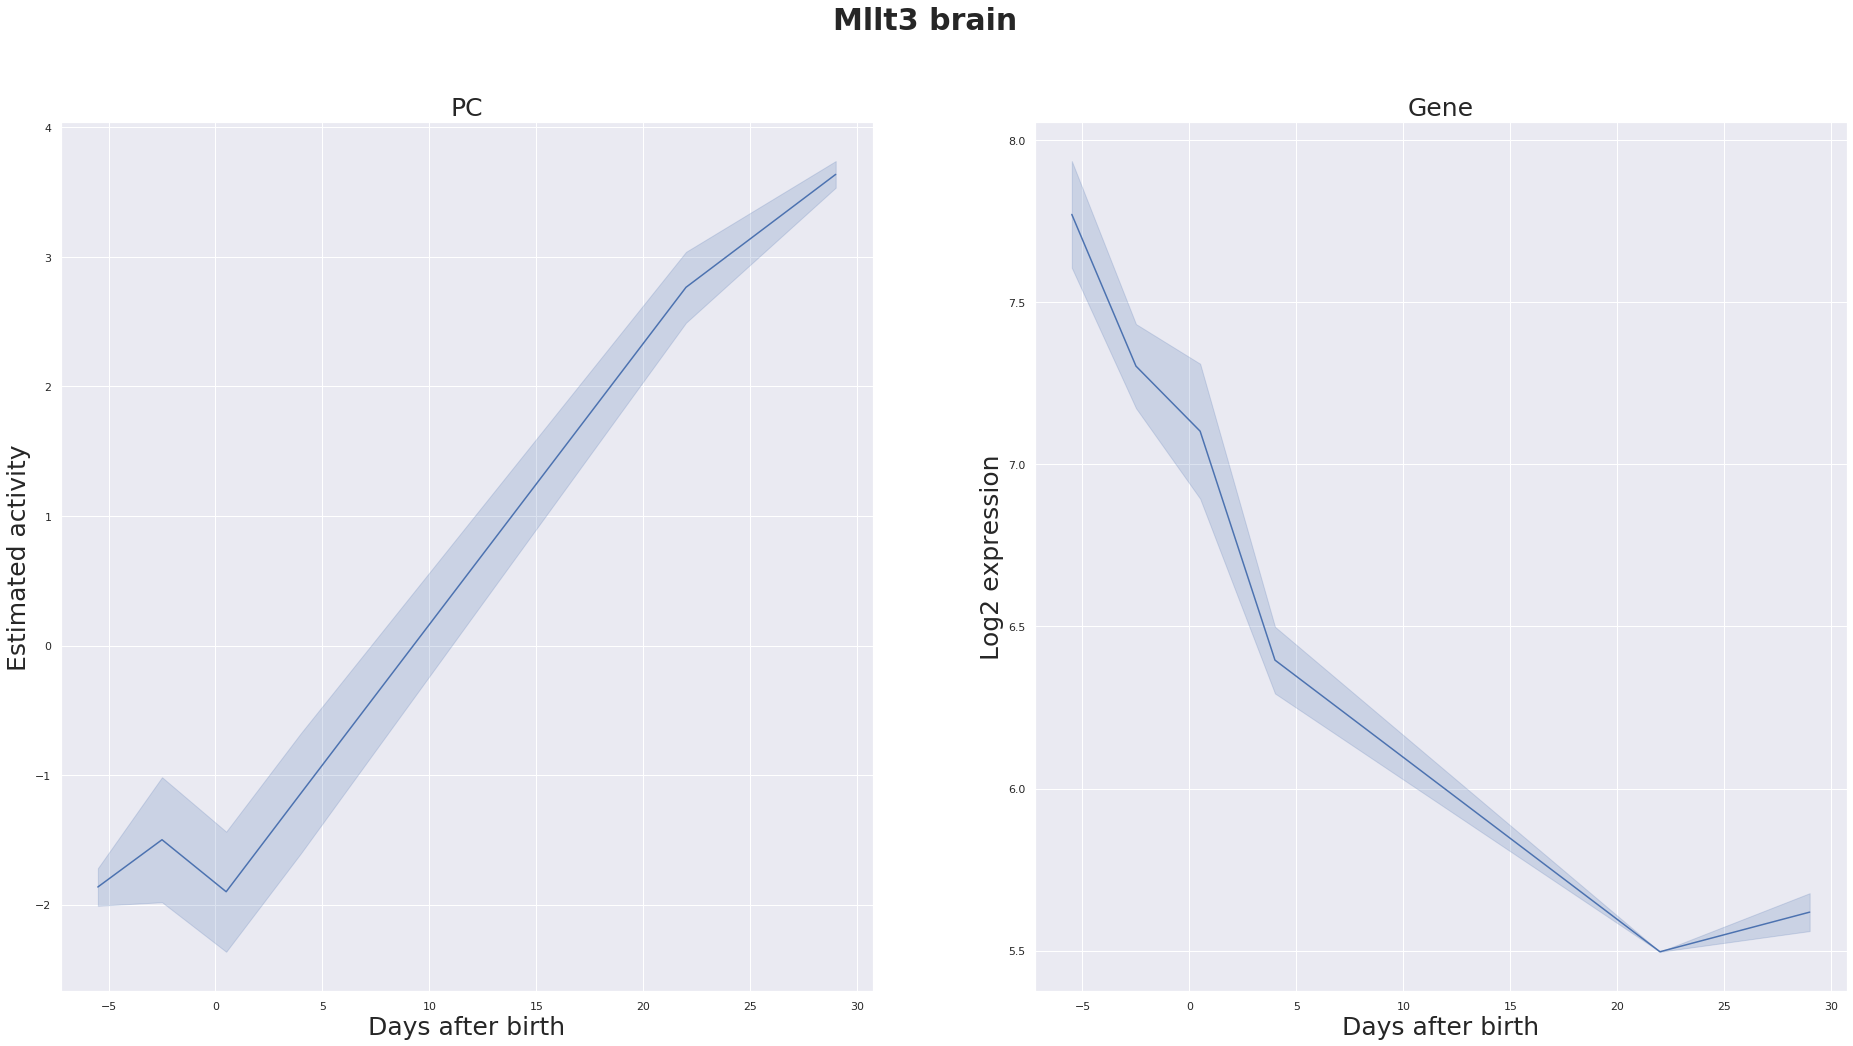
\includegraphics[width=6cm,height=3cm]{Figures&amp;Cover/Activity_Mllt3_brain_NonePCremoved_filtering_False.png}
    \vspace{0.25cm}
    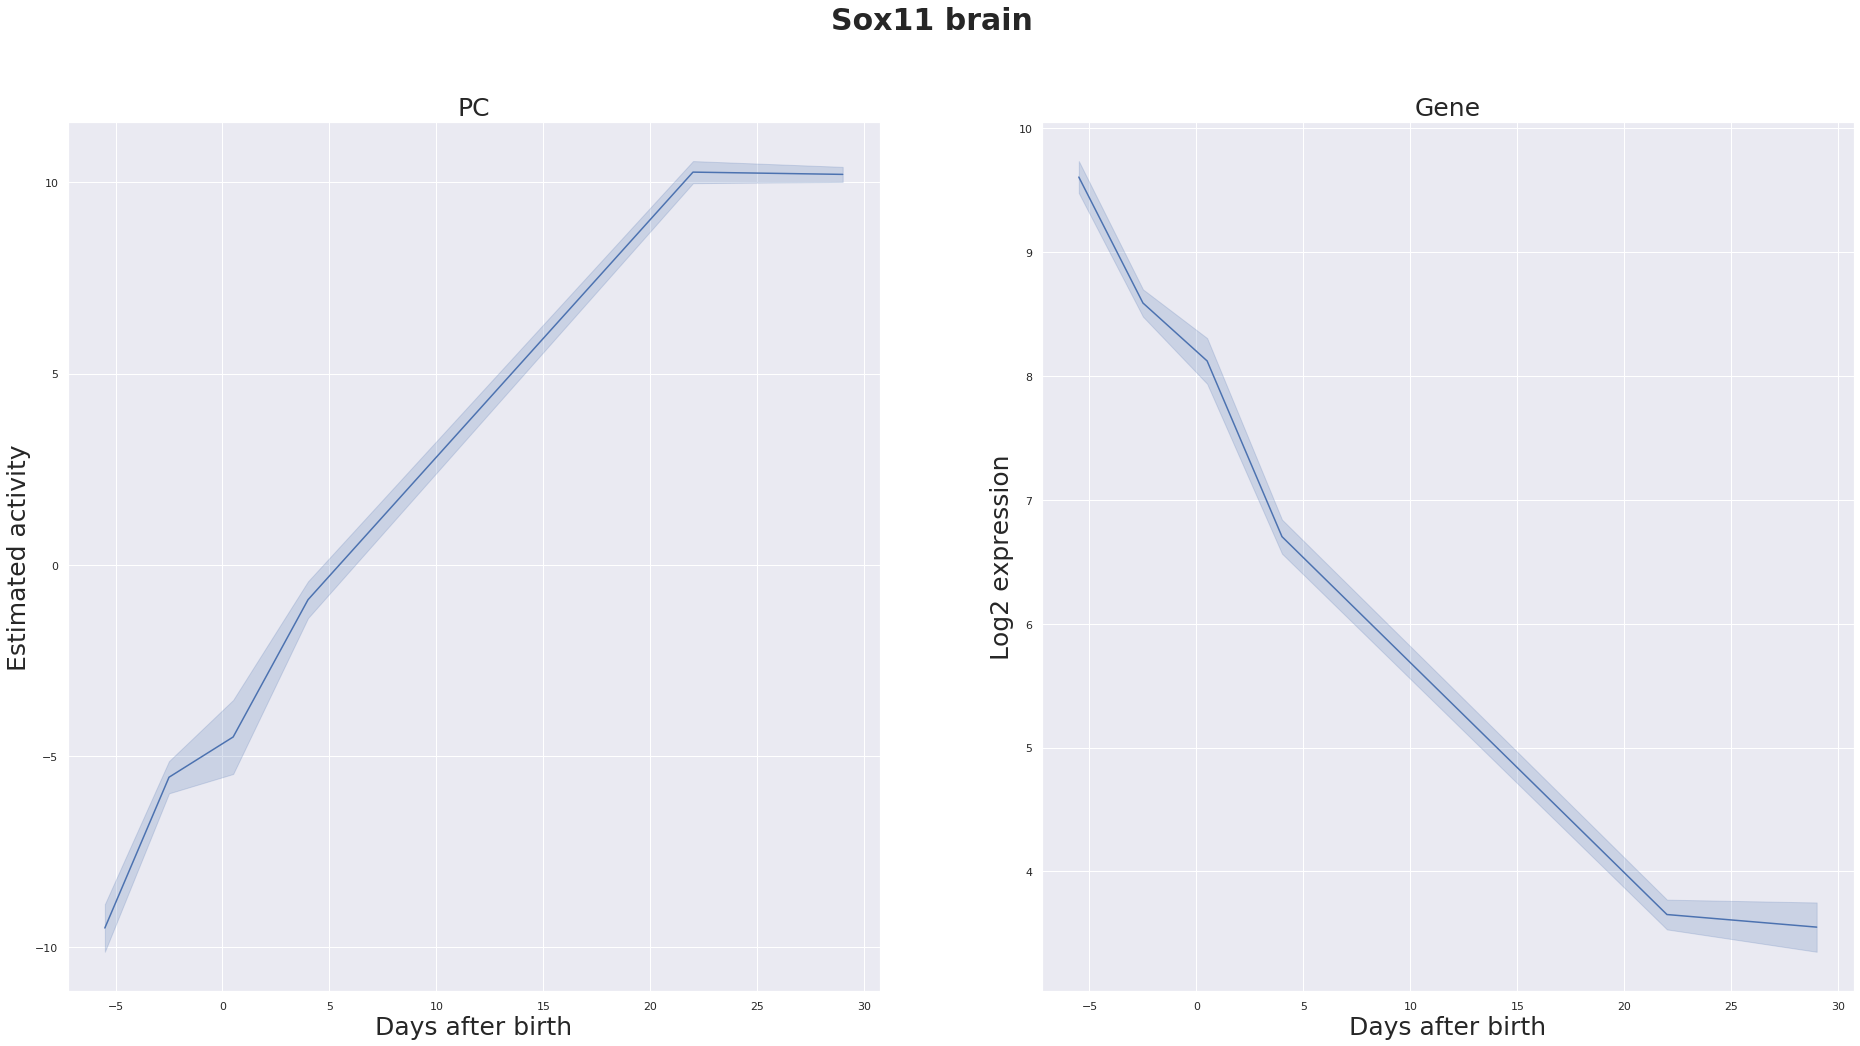
\includegraphics[width=6cm,height=3cm]{Figures&amp;Cover/Activity_Sox11_brain_NonePCremoved_filtering_False.png}
    \caption{\textbf{Estimated activities of Tal1, Lmo2, Ncapg, Ikzf1, Top2a, Klf9, Brca1, Mllt3 and Sox11 in mouse brains as a functions of the mices' age.} The activities were estimated by the first \ac{PC} of the mRNA expression data of the genes each \ac{TF} is likely to regulate (left figure of each pair) as well as directly through the transcription of the genes coding for each \ac{TF}, as log2-transformed \ac{RPM} transcript counts (right figure of each pair).}
    \label{fig:BrainEsts1}
\end{figure}    
    
\begin{figure}
    \centering
    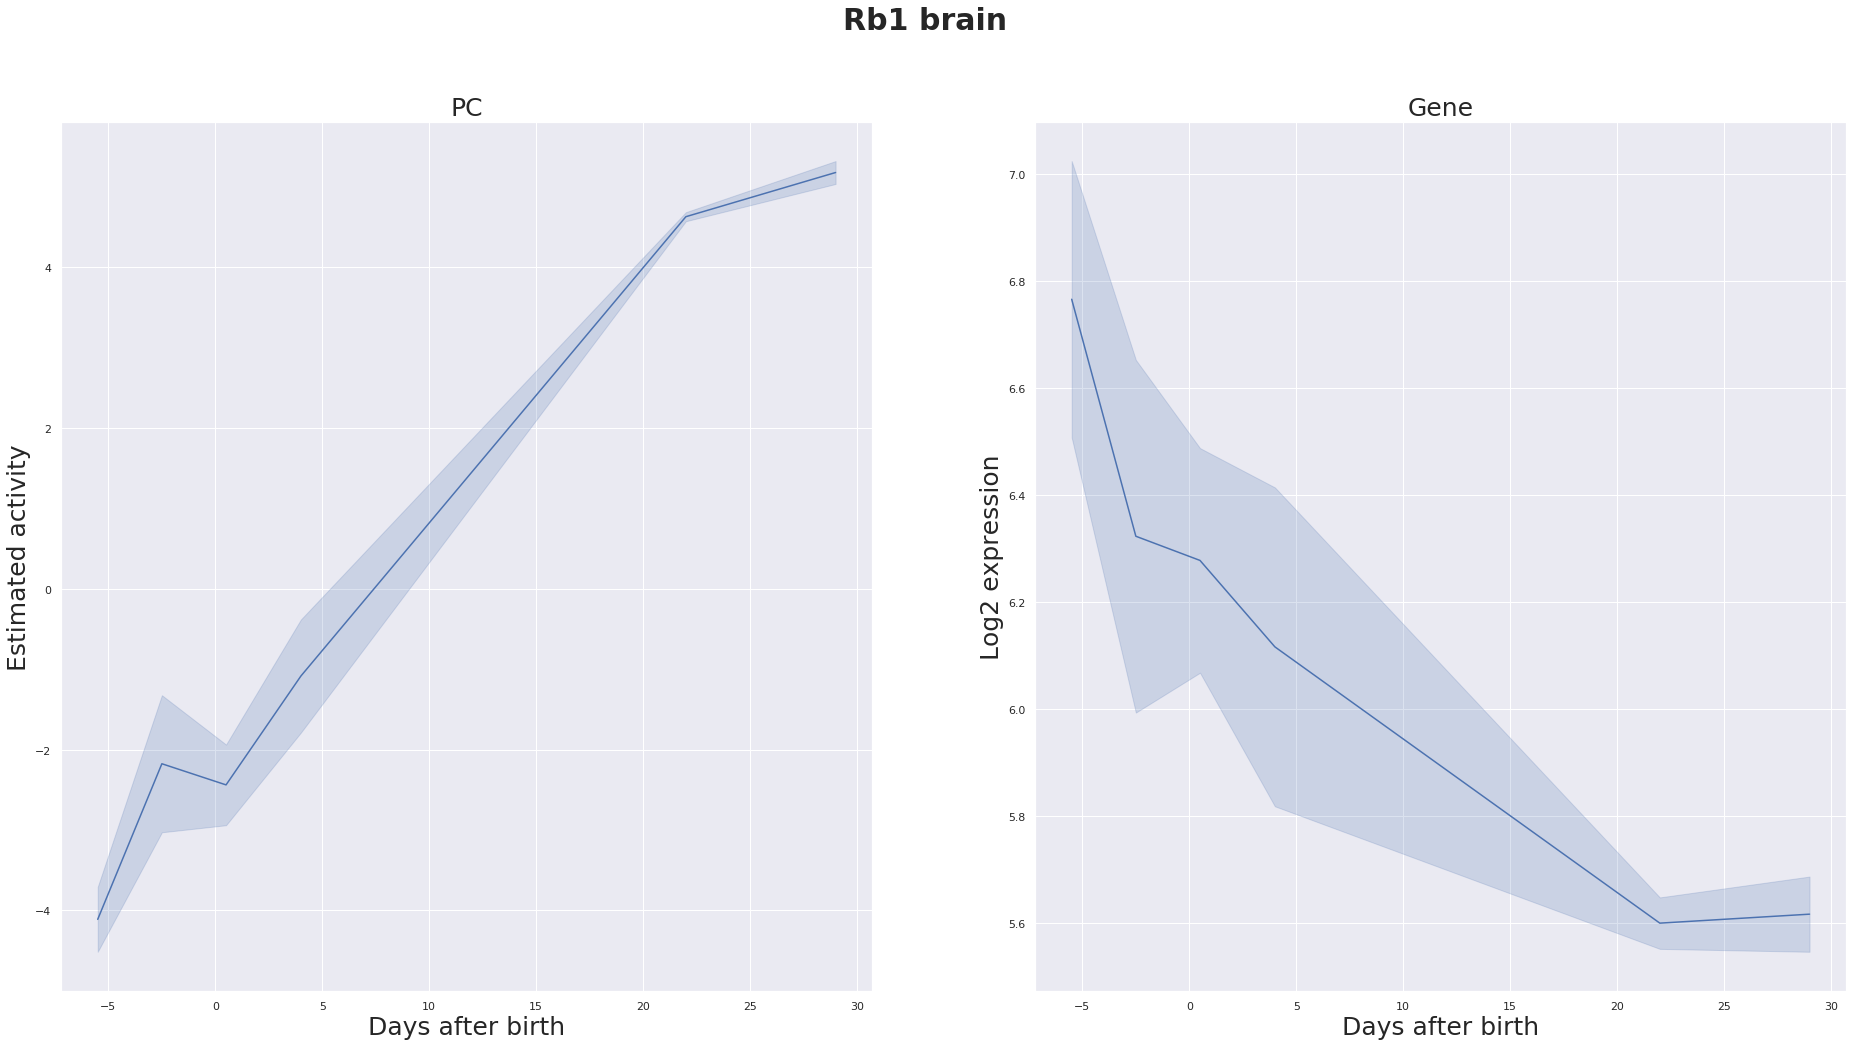
\includegraphics[width=6cm,height=3cm]{Figures&amp;Cover/Activity_Rb1_brain_NonePCremoved_filtering_False.png}
    \hspace{0.25cm}
    \vspace{0.25cm}
    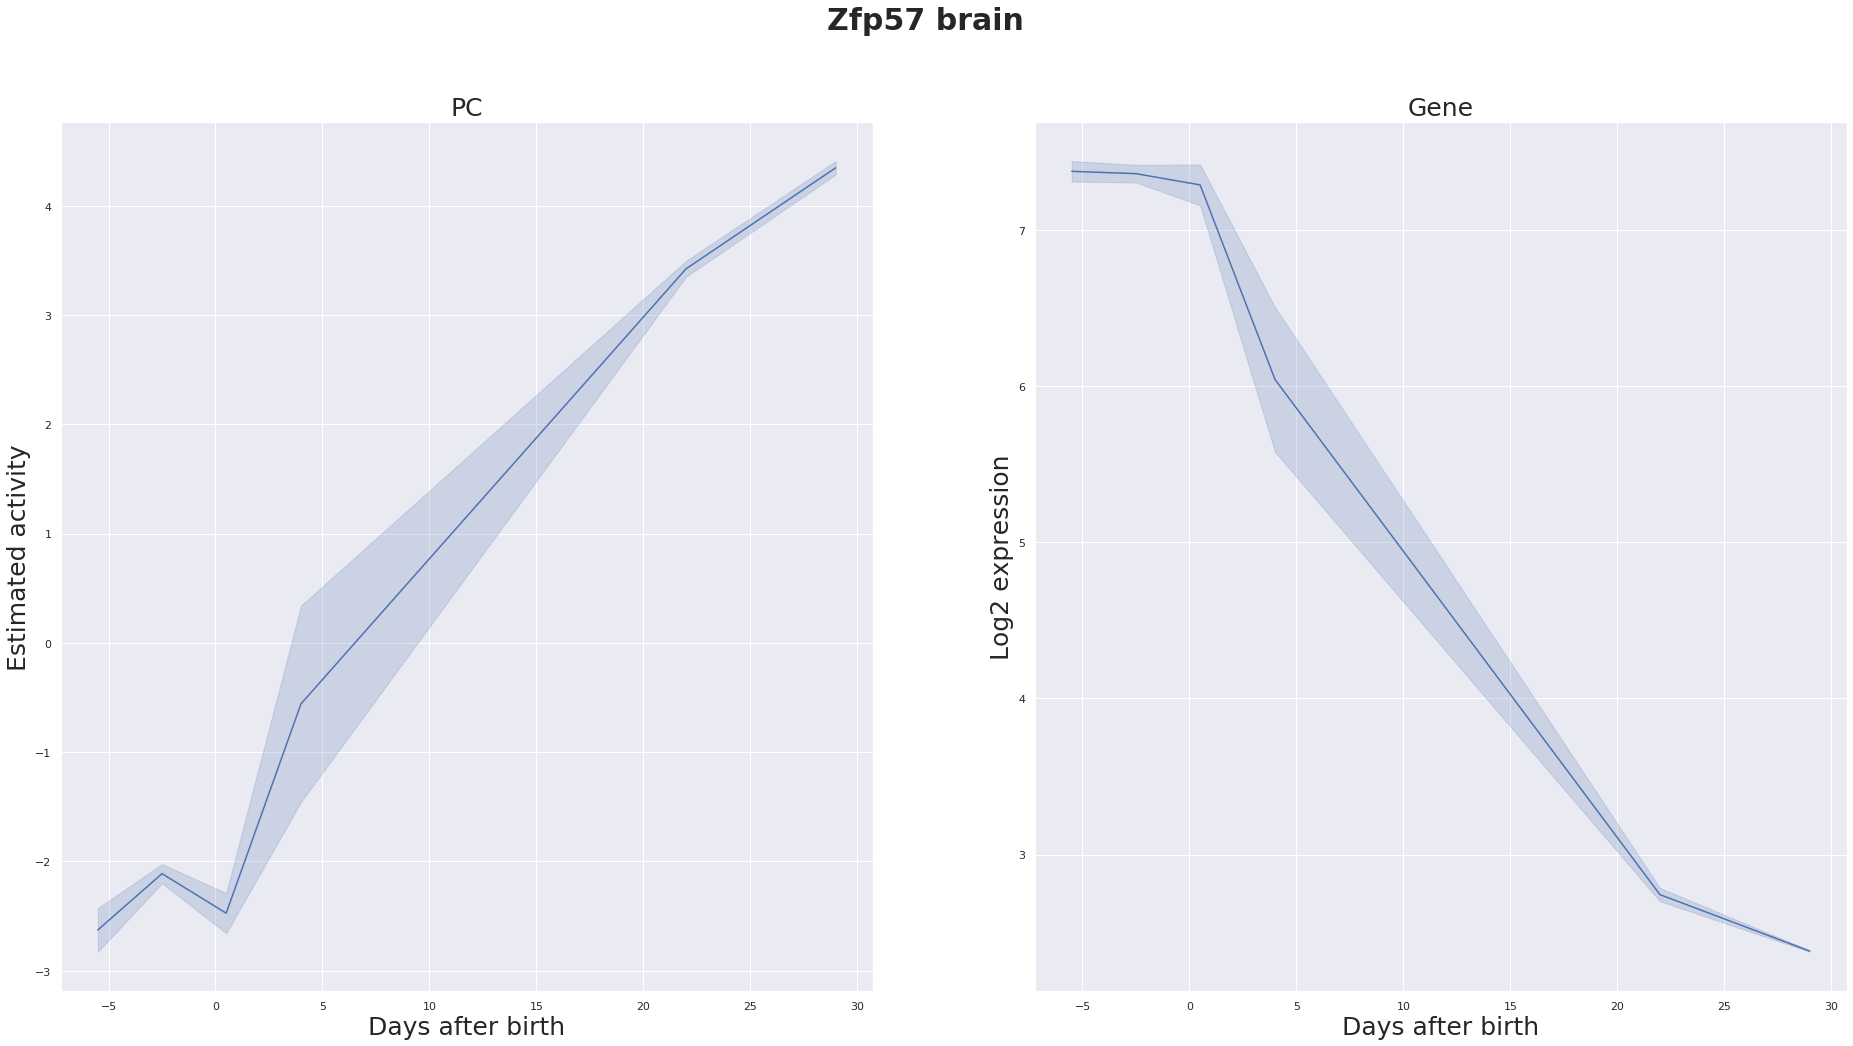
\includegraphics[width=6cm,height=3cm]{Figures&amp;Cover/Activity_Zfp57_brain_NonePCremoved_filtering_False.png}
    \vspace{0.25cm}
    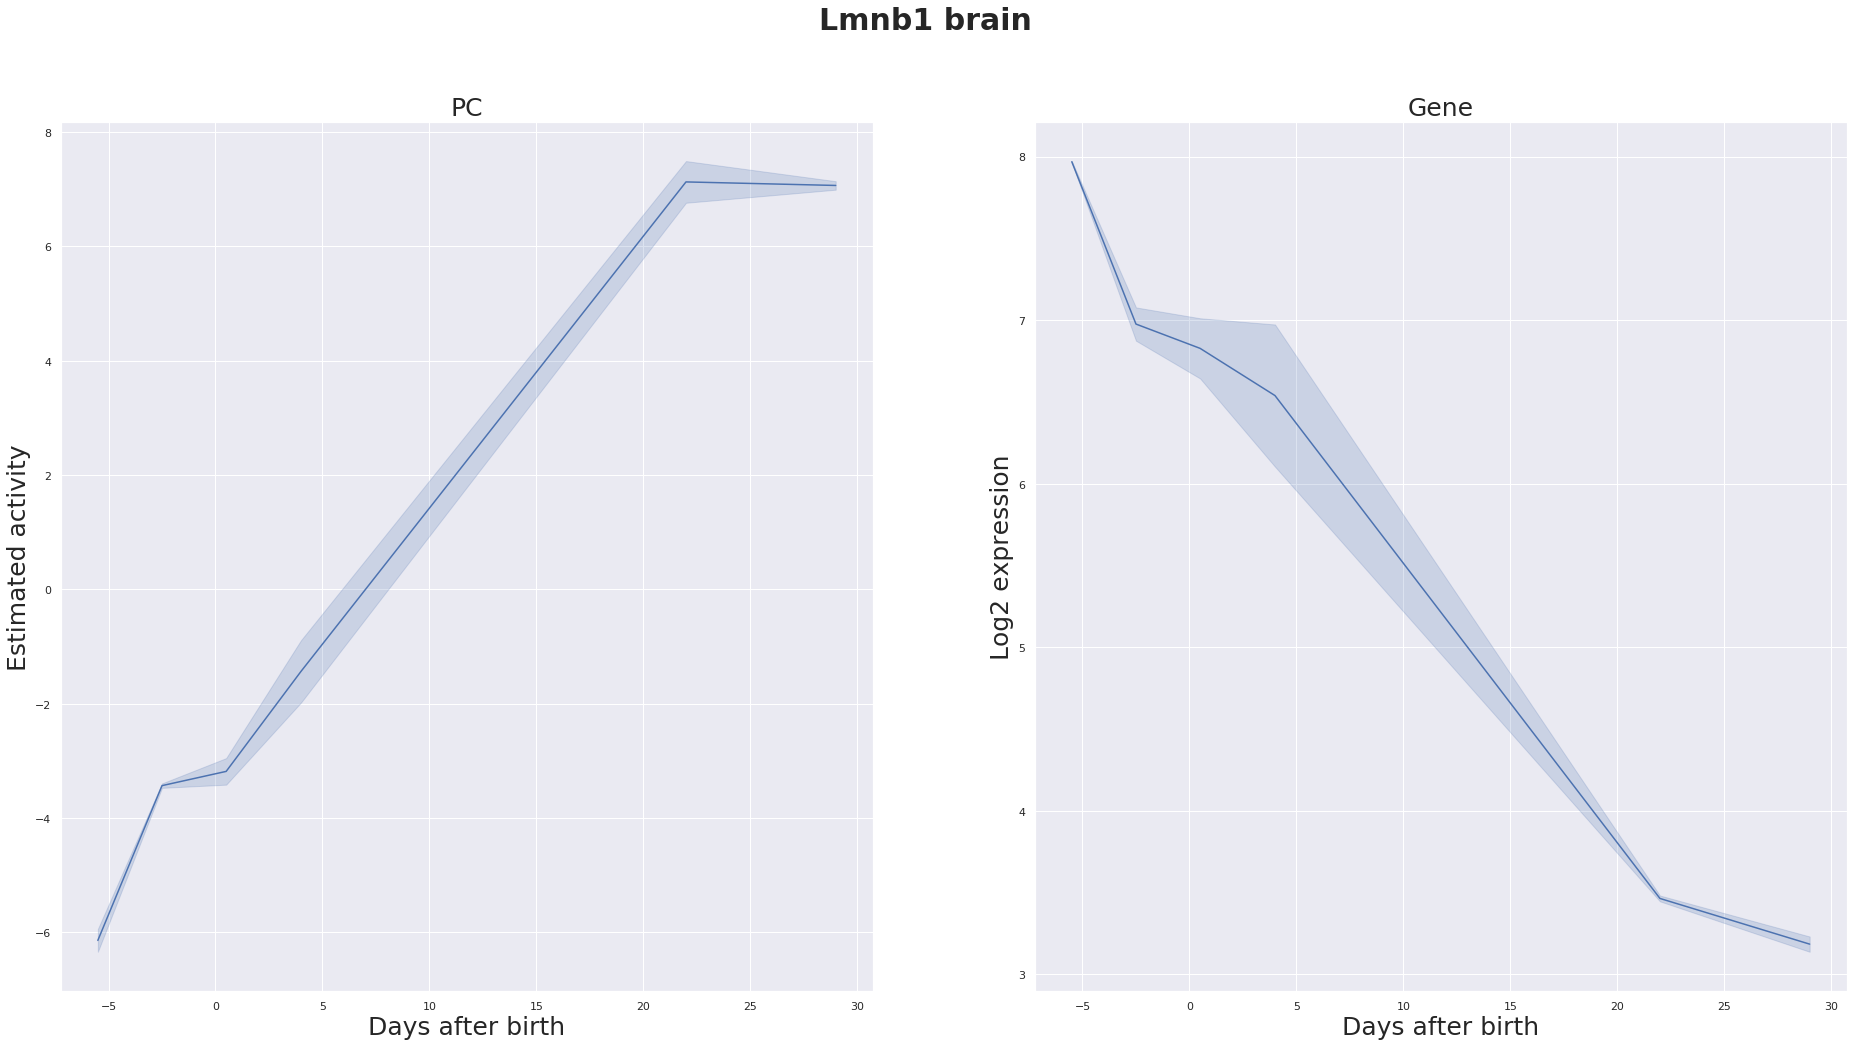
\includegraphics[width=6cm,height=3cm]{Figures&amp;Cover/Activity_Lmnb1_brain_NonePCremoved_filtering_False.png}
    \hspace{0.25cm}
    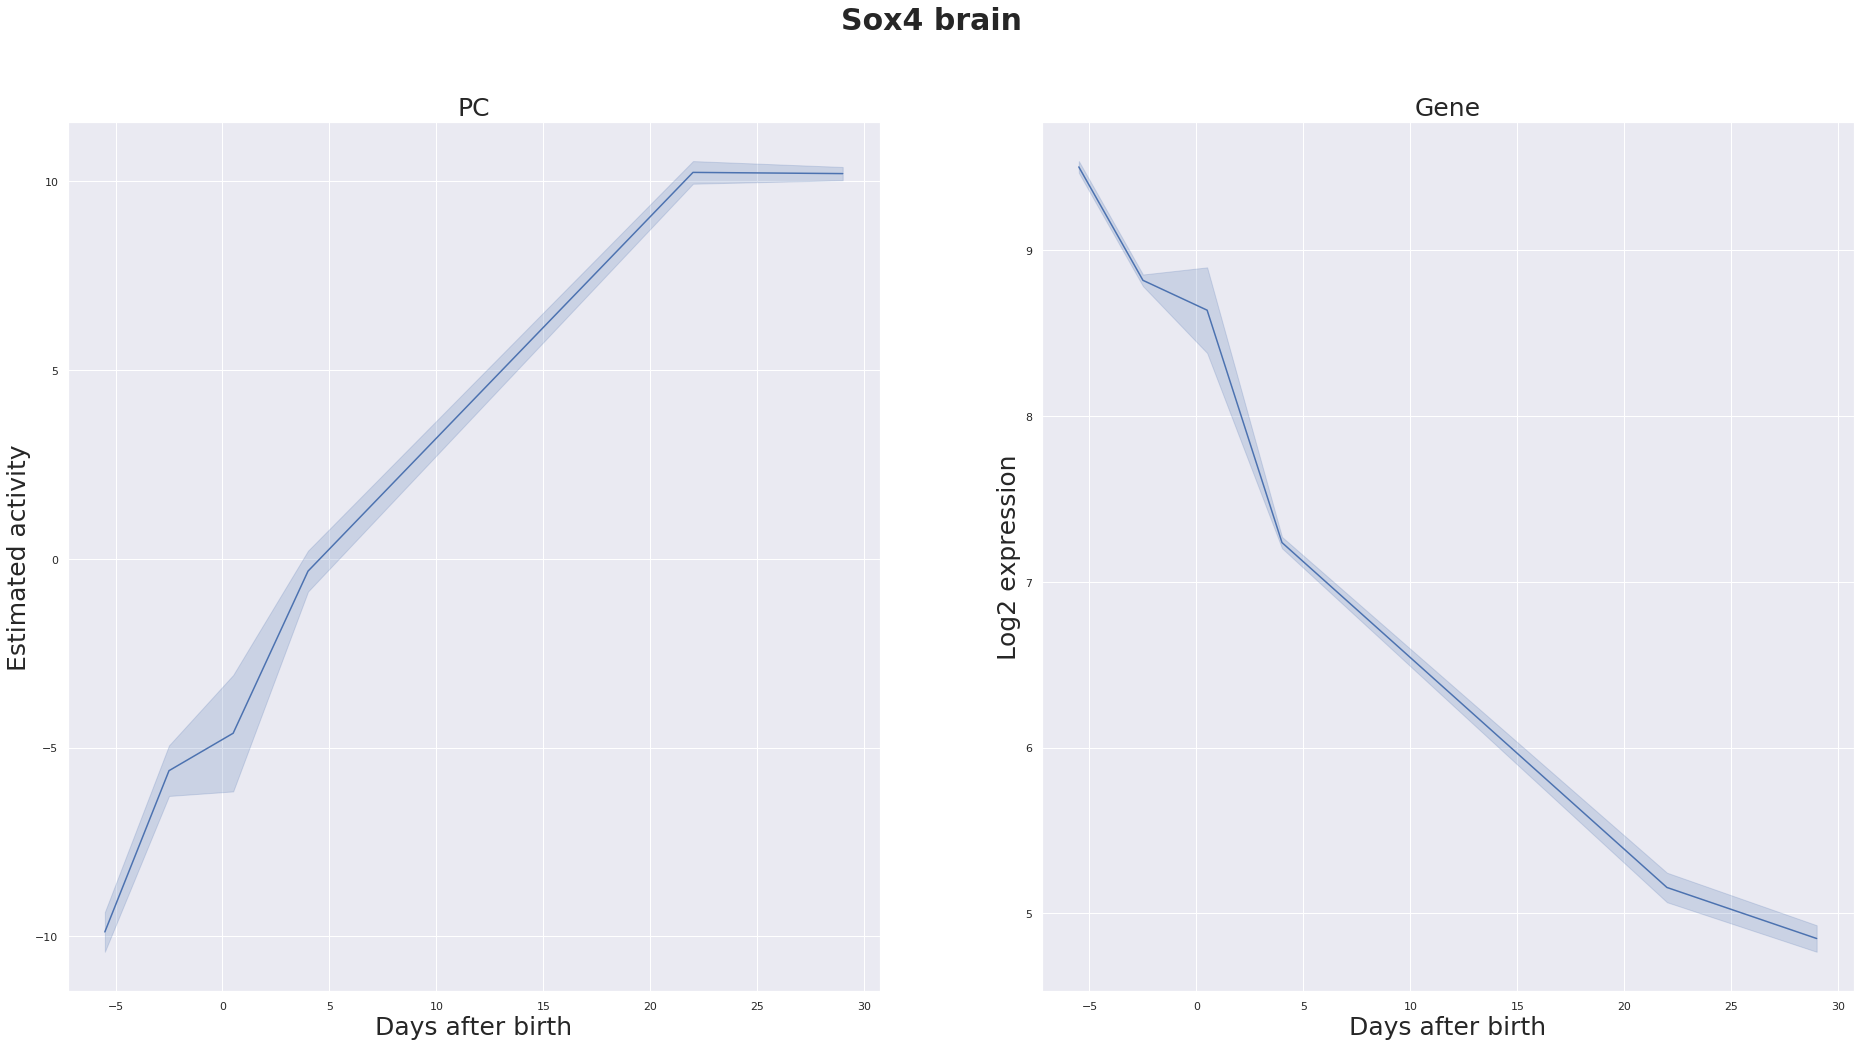
\includegraphics[width=6cm,height=3cm]{Figures&amp;Cover/Activity_Sox4_brain_NonePCremoved_filtering_False.png}
    \vspace{0.25cm}
    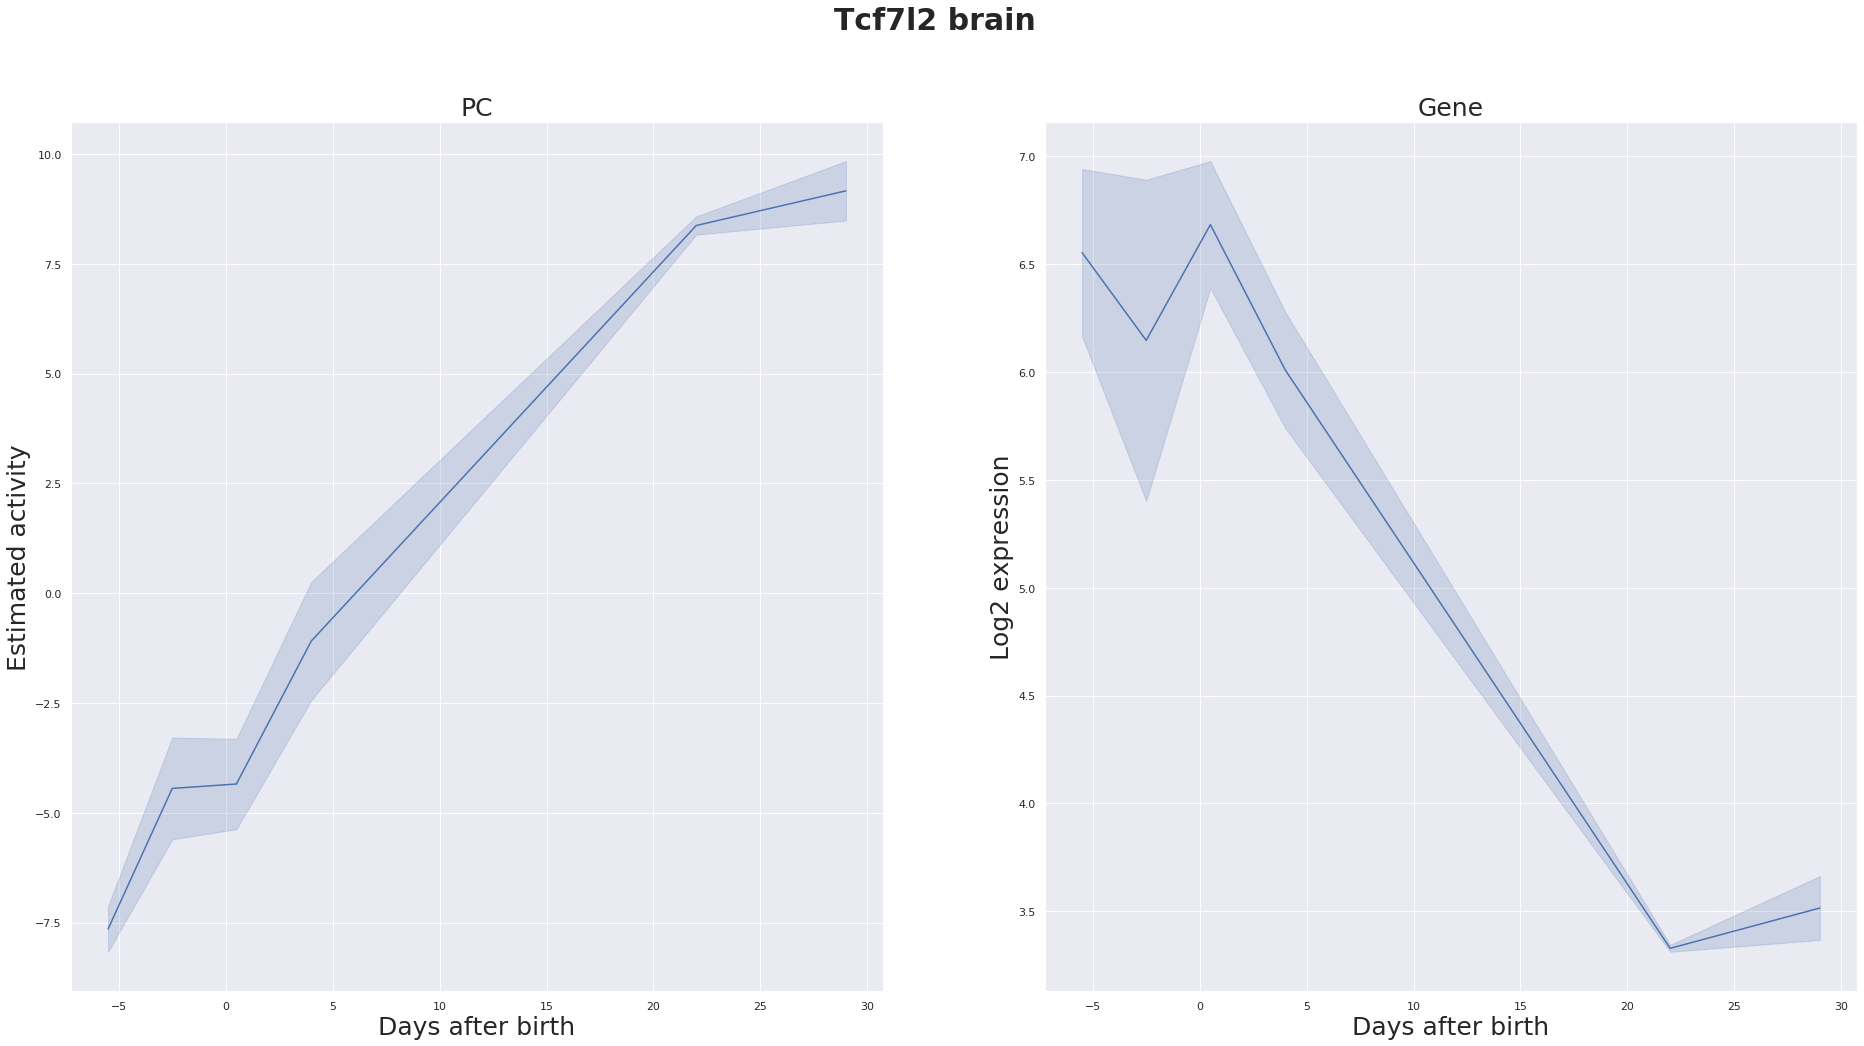
\includegraphics[width=6cm,height=3cm]{Figures&amp;Cover/Activity_Tcf7l2_brain_NonePCremoved_filtering_False.png}
    \hspace{0.25cm}
    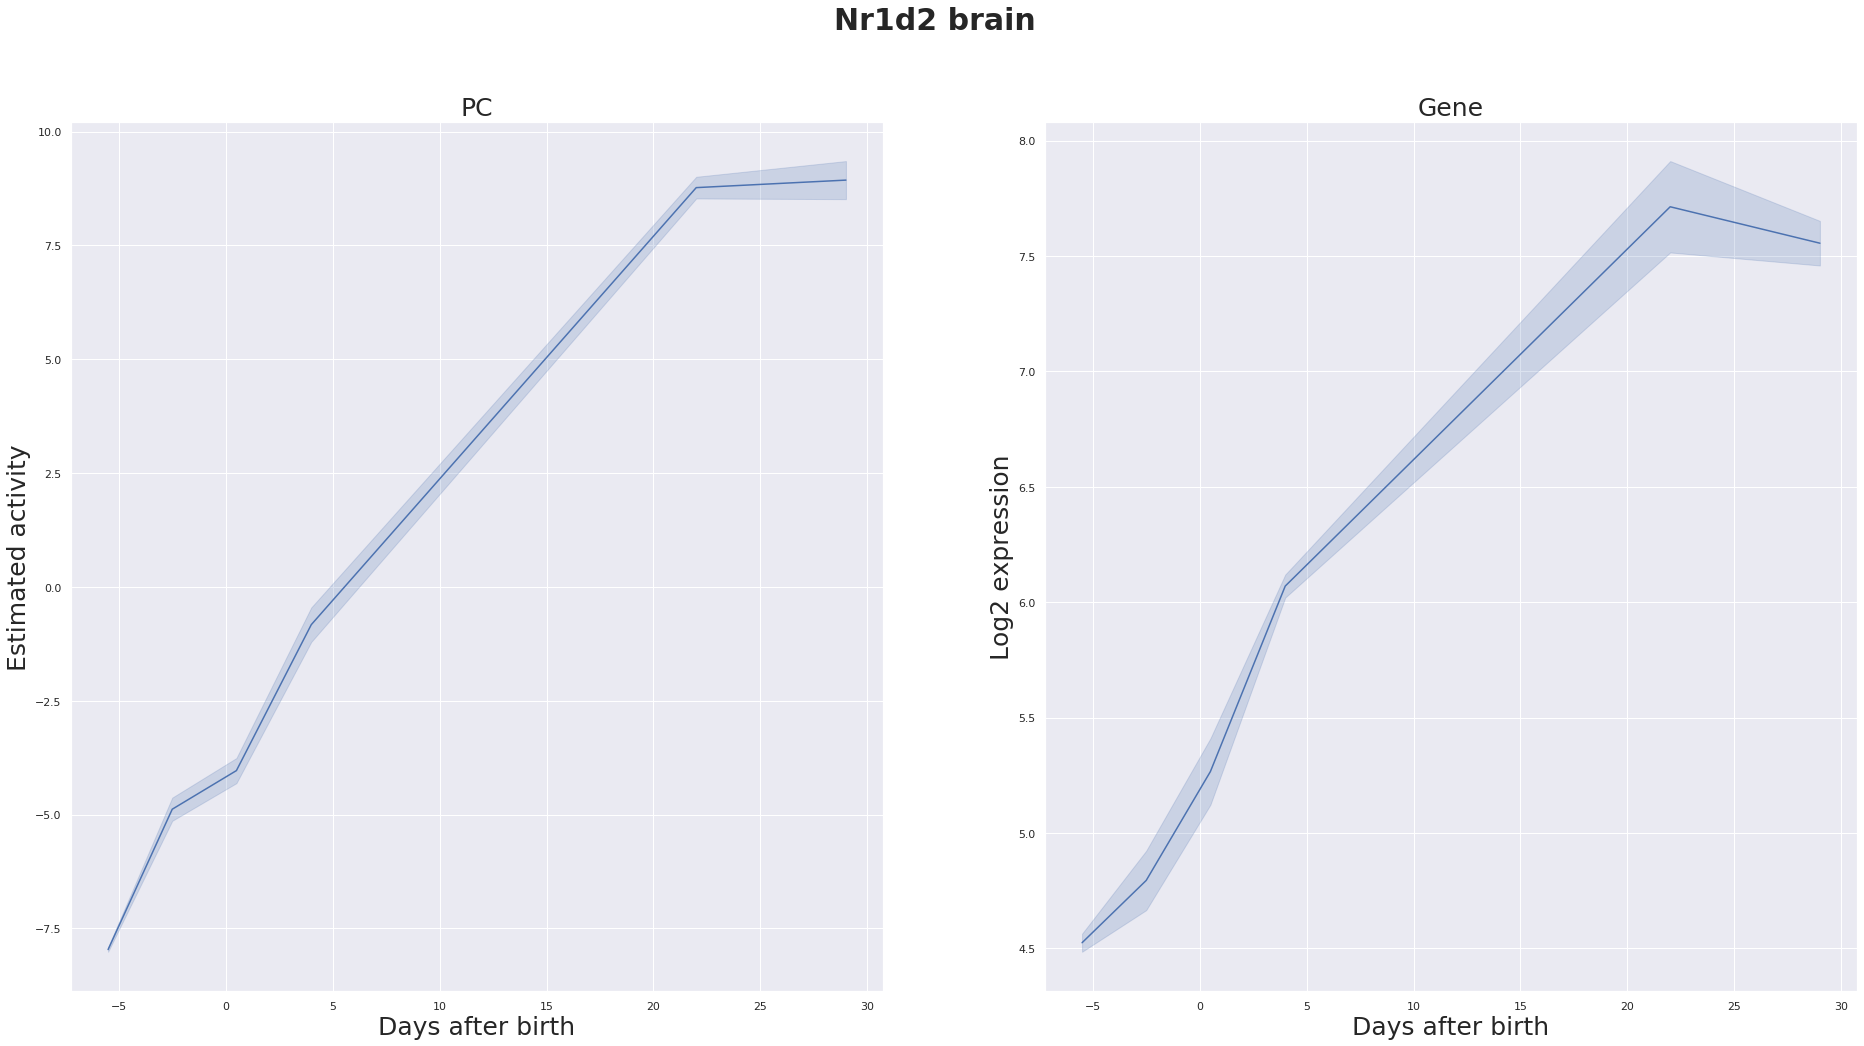
\includegraphics[width=6cm,height=3cm]{Figures&amp;Cover/Activity_Nr1d2_brain_NonePCremoved_filtering_False.png}
    \vspace{0.25cm}
    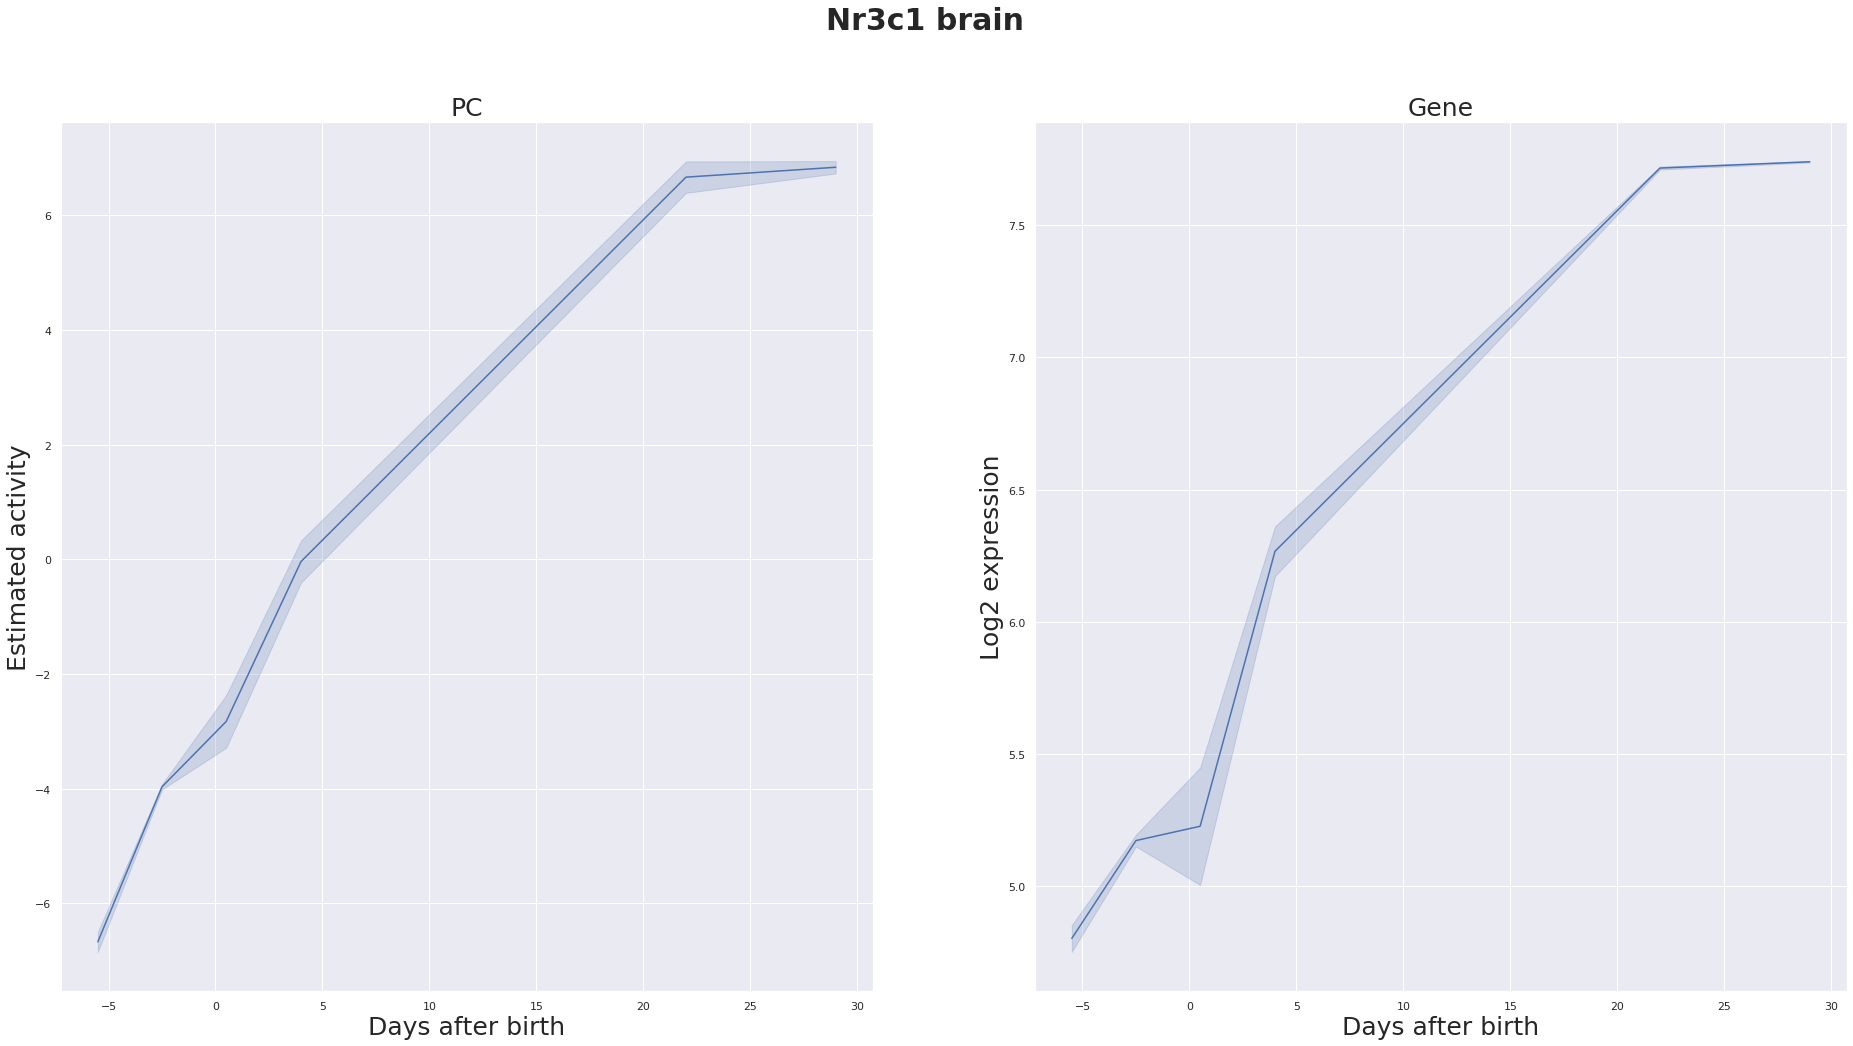
\includegraphics[width=6cm,height=3cm]{Figures&amp;Cover/Activity_Nr3c1_brain_NonePCremoved_filtering_False.png}
    \hspace{0.25cm}
    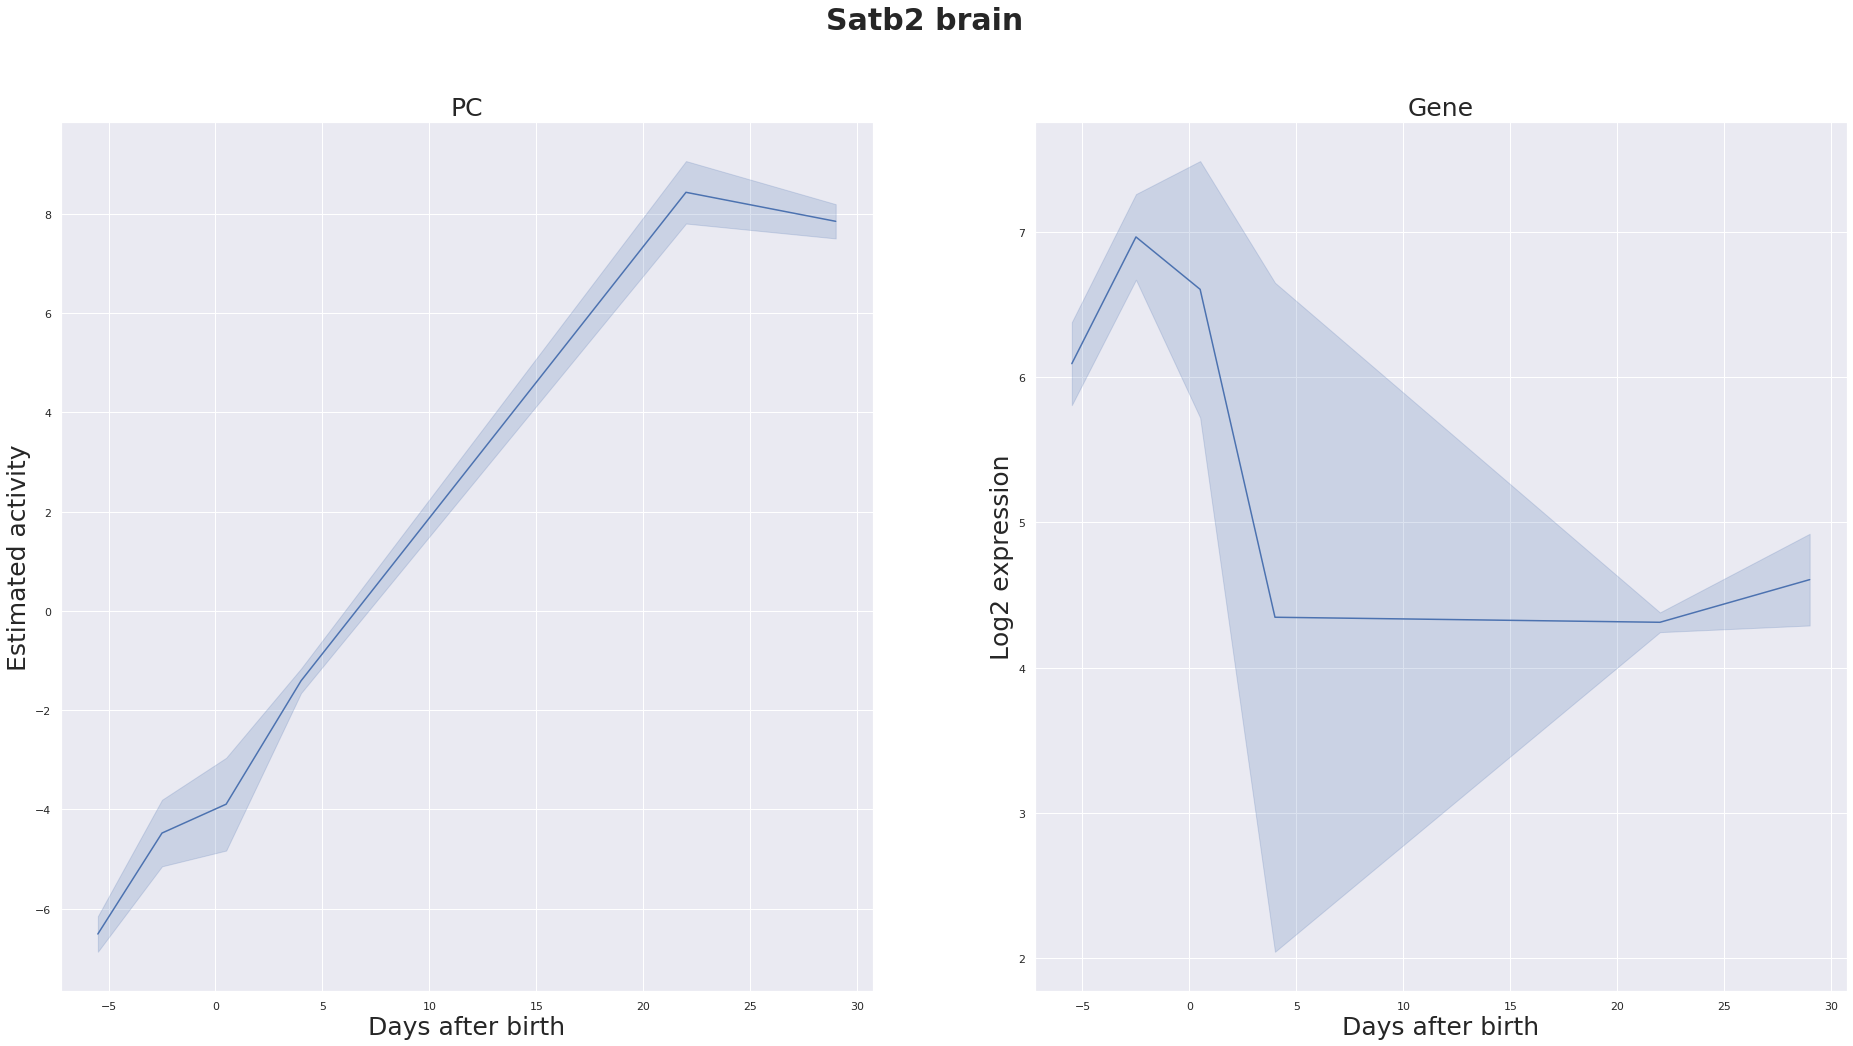
\includegraphics[width=6cm,height=3cm]{Figures&amp;Cover/Activity_Satb2_brain_NonePCremoved_filtering_False.png}
    \caption{\textbf{Estimated activities of Rb1, Zfp57, Lmnb1, Sox4, Tc7l2, Nr1d2, Nr3c1 and Satb2 in mouse brains as a functions of the mices' age.} The activities were estimated by the first \ac{PC} of the mRNA expression data of the genes each \ac{TF} is likely to regulate (left figure of each pair) as well as directly through the transcription of the genes coding for each \ac{TF}, as log2-transformed \ac{RPM} transcript counts (right figure of each pair).}
    \label{fig:BrainEsts2}
\end{figure}

\begin{figure}
    \centering
    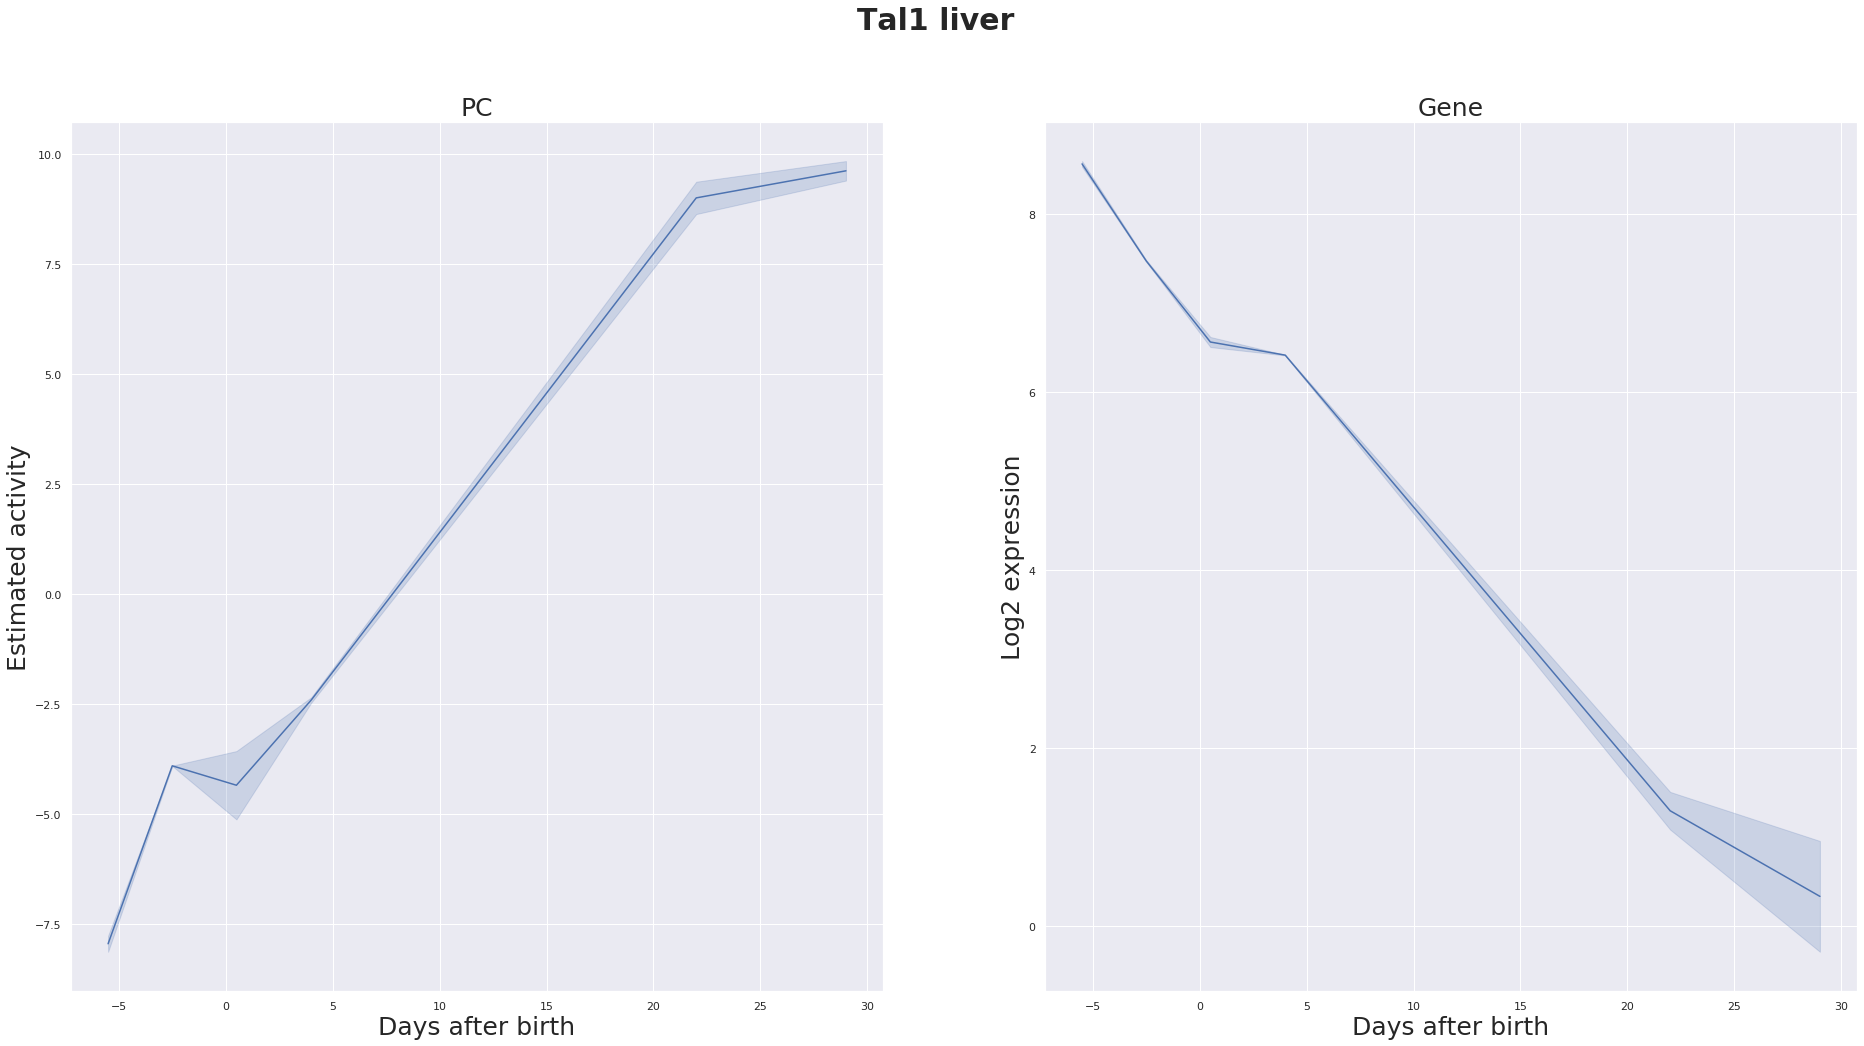
\includegraphics[width=6cm,height=3cm]{Figures&amp;Cover/Activity_Tal1_liver_NonePCremoved_filtering_False.png}
    \hspace{0.25cm}
    \vspace{0.25cm}
    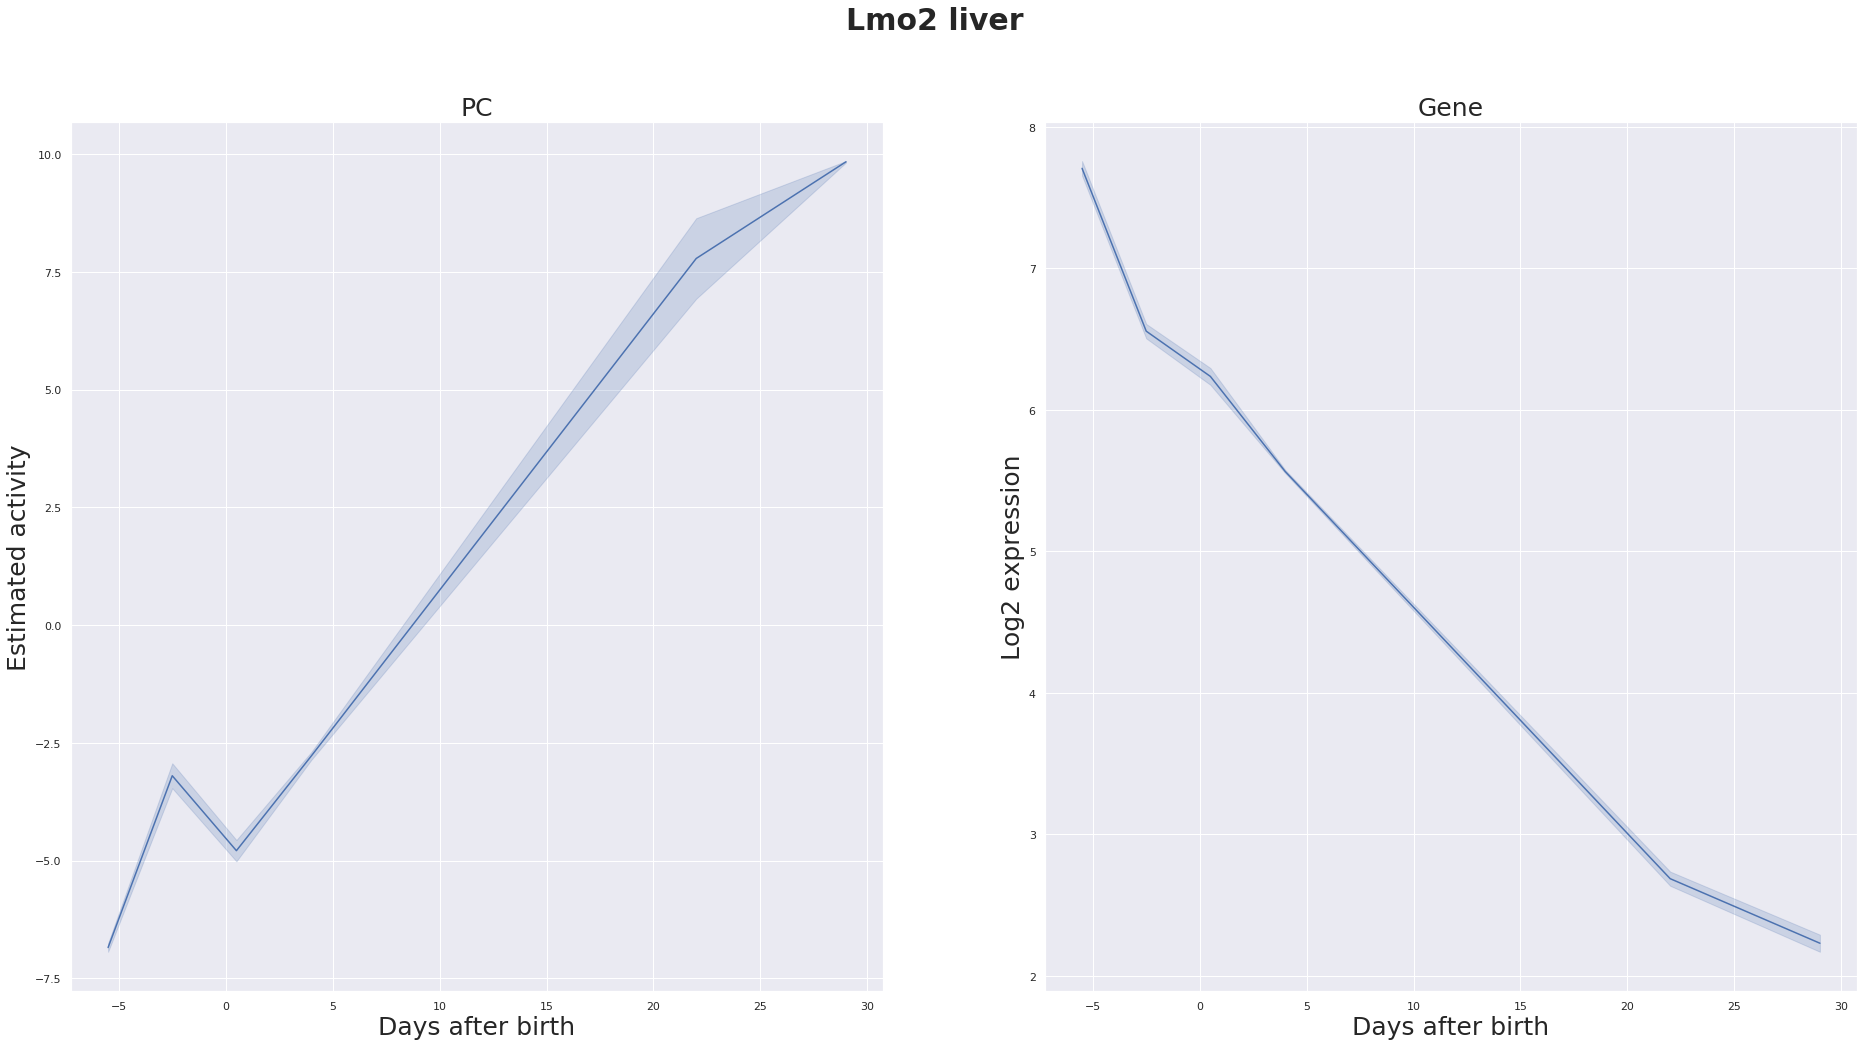
\includegraphics[width=6cm,height=3cm]{Figures&amp;Cover/Activity_Lmo2_liver_NonePCremoved_filtering_False.png}
    \vspace{0.25cm}
    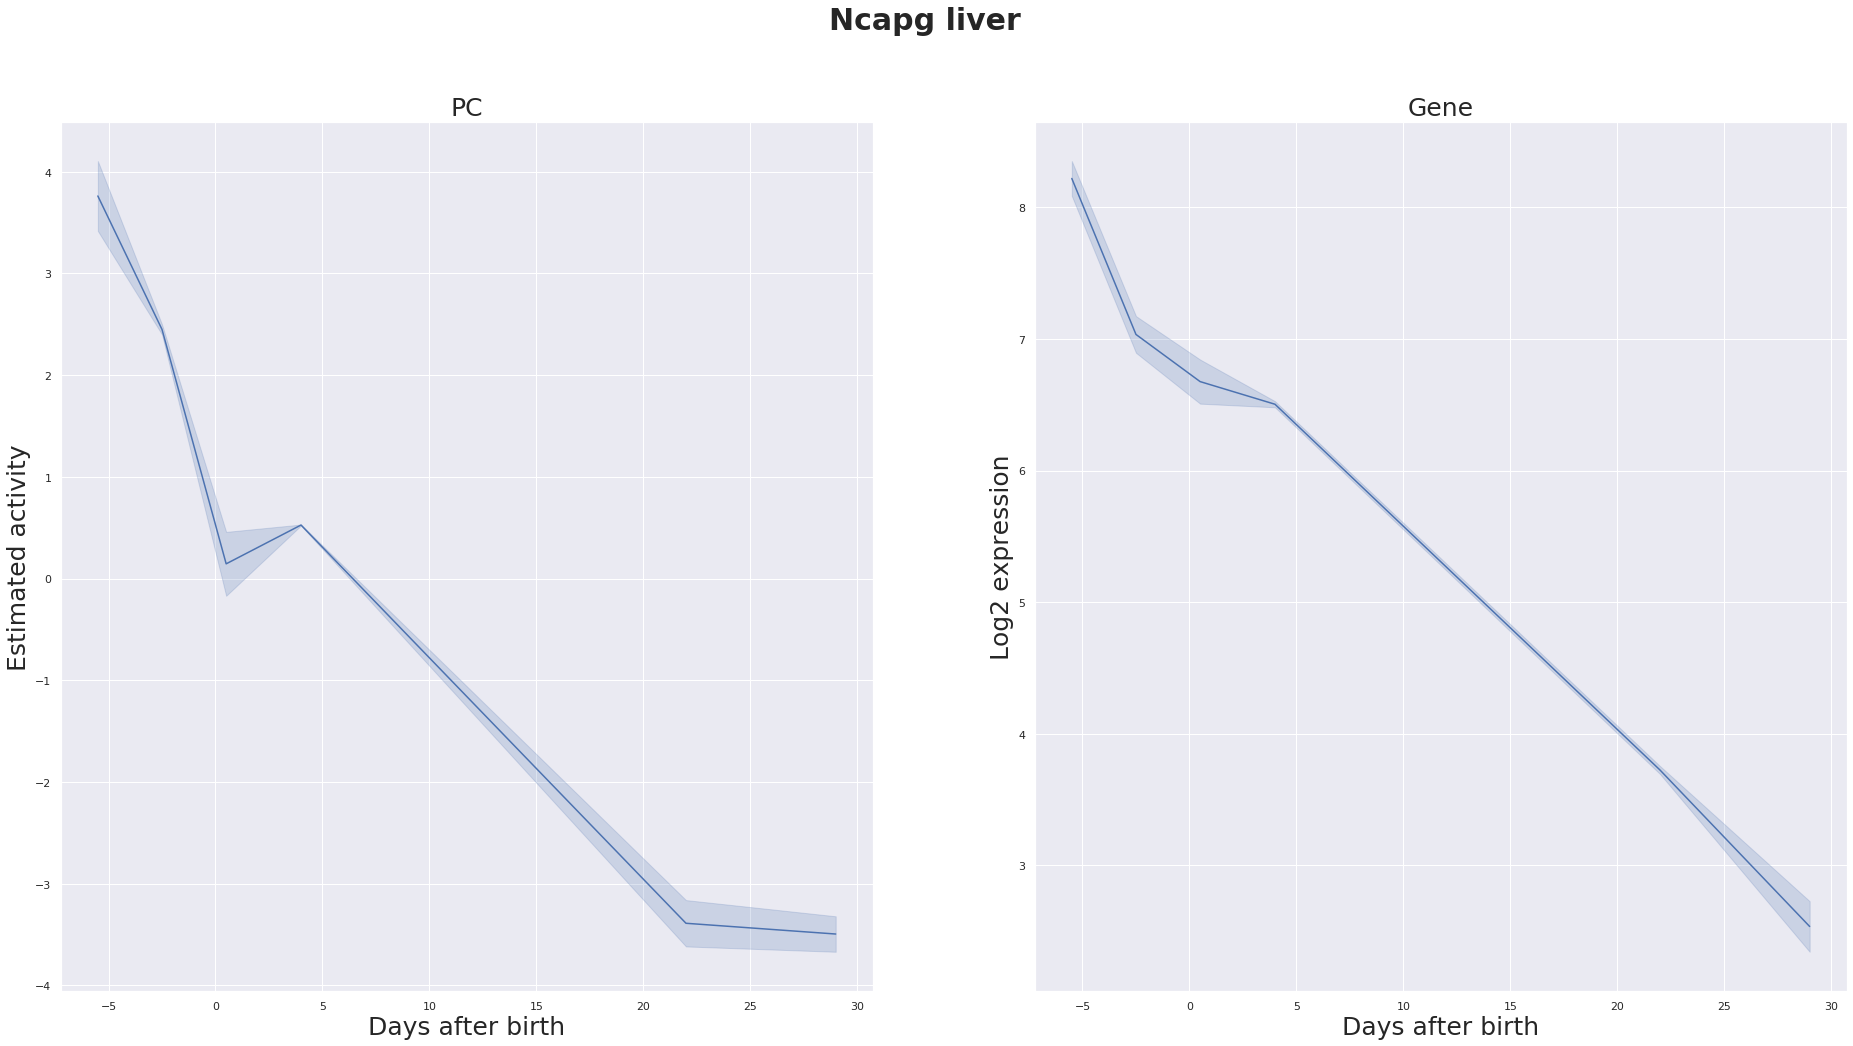
\includegraphics[width=6cm,height=3cm]{Figures&amp;Cover/Activity_Ncapg_liver_NonePCremoved_filtering_False.png}
    \hspace{0.25cm}
    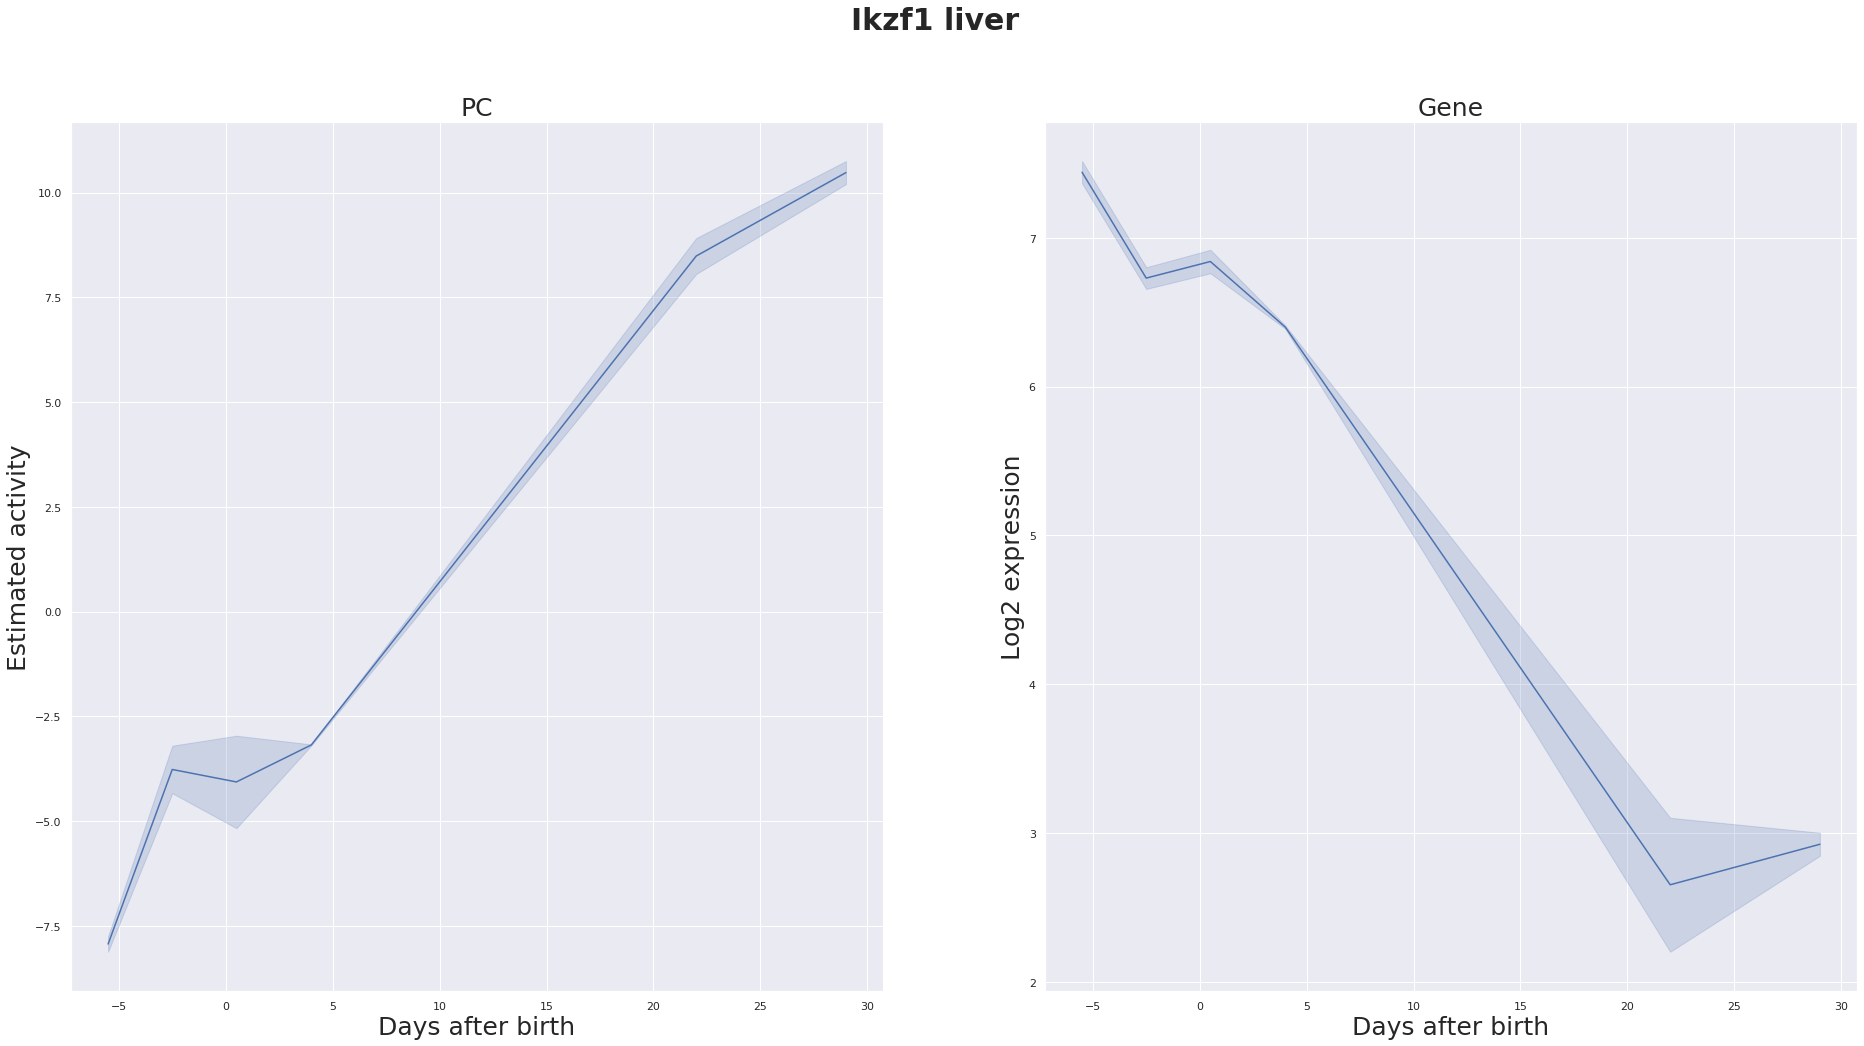
\includegraphics[width=6cm,height=3cm]{Figures&amp;Cover/Activity_Ikzf1_liver_NonePCremoved_filtering_False.png}
    \vspace{0.25cm}
    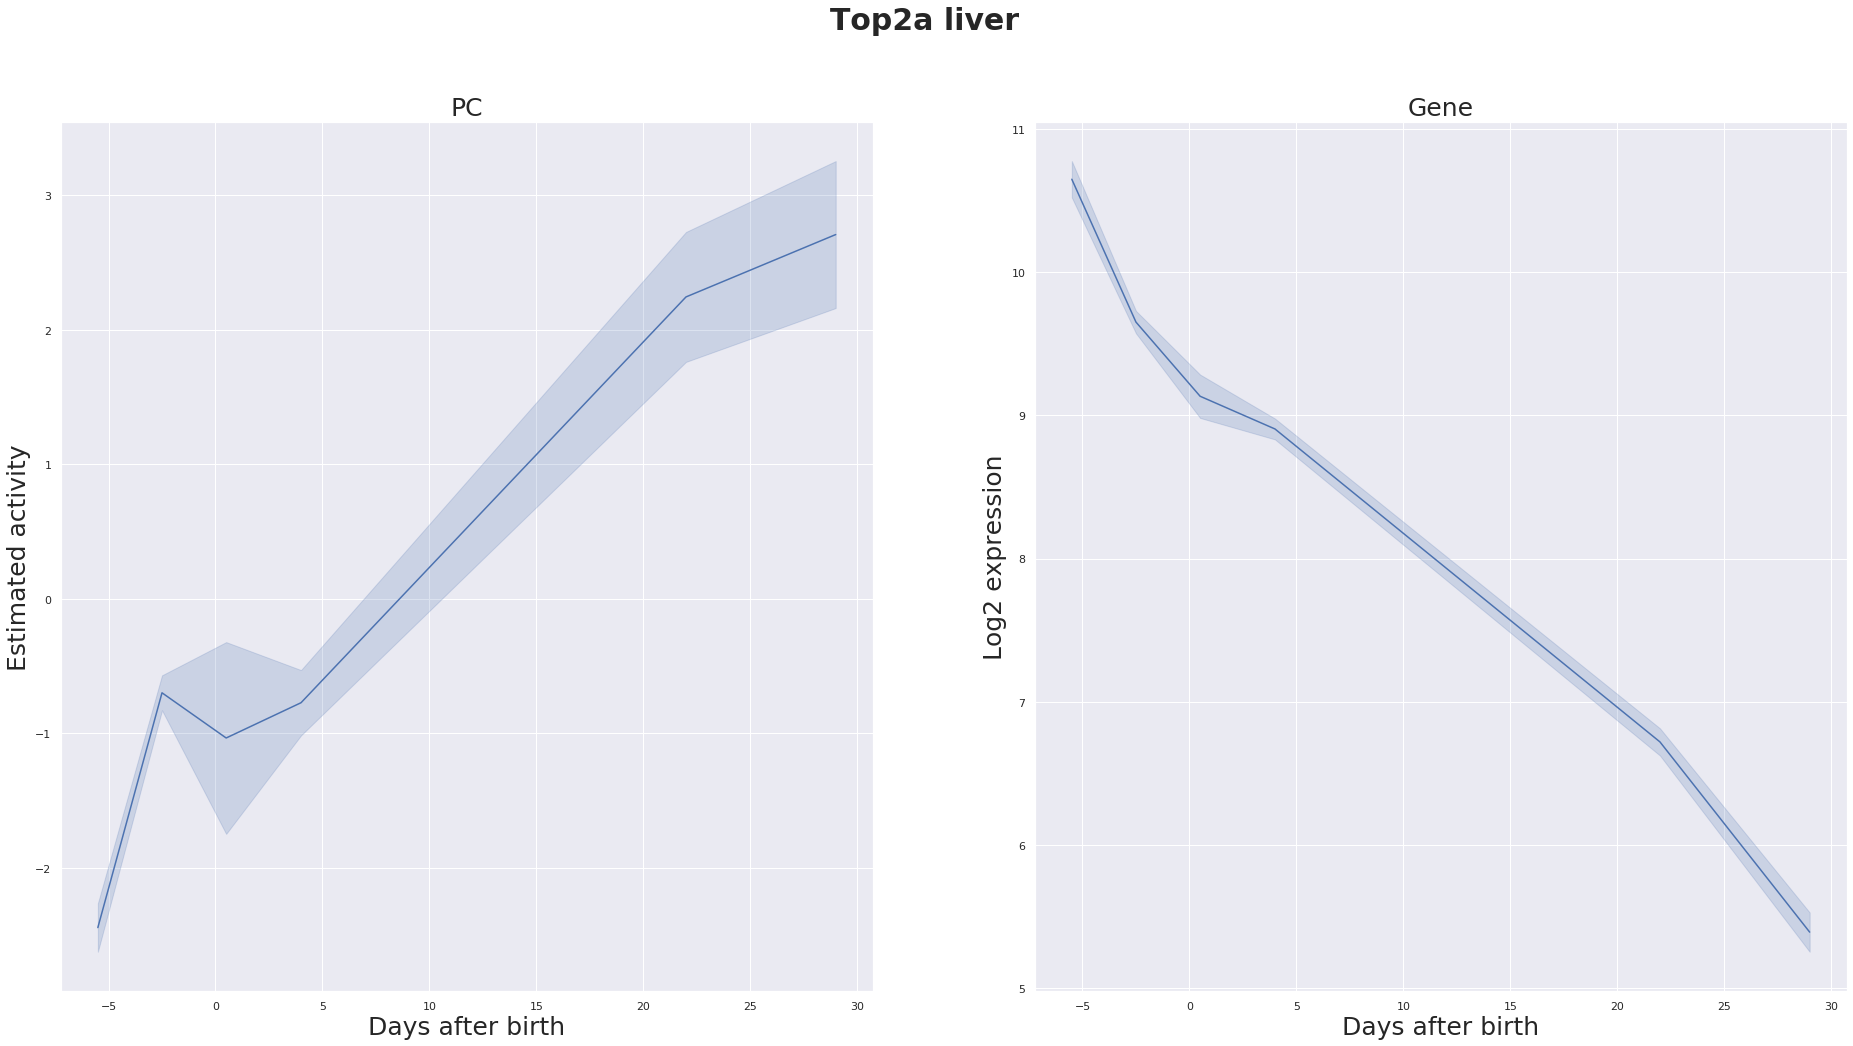
\includegraphics[width=6cm,height=3cm]{Figures&amp;Cover/Activity_Top2a_liver_NonePCremoved_filtering_False.png}
    \hspace{0.25cm}
    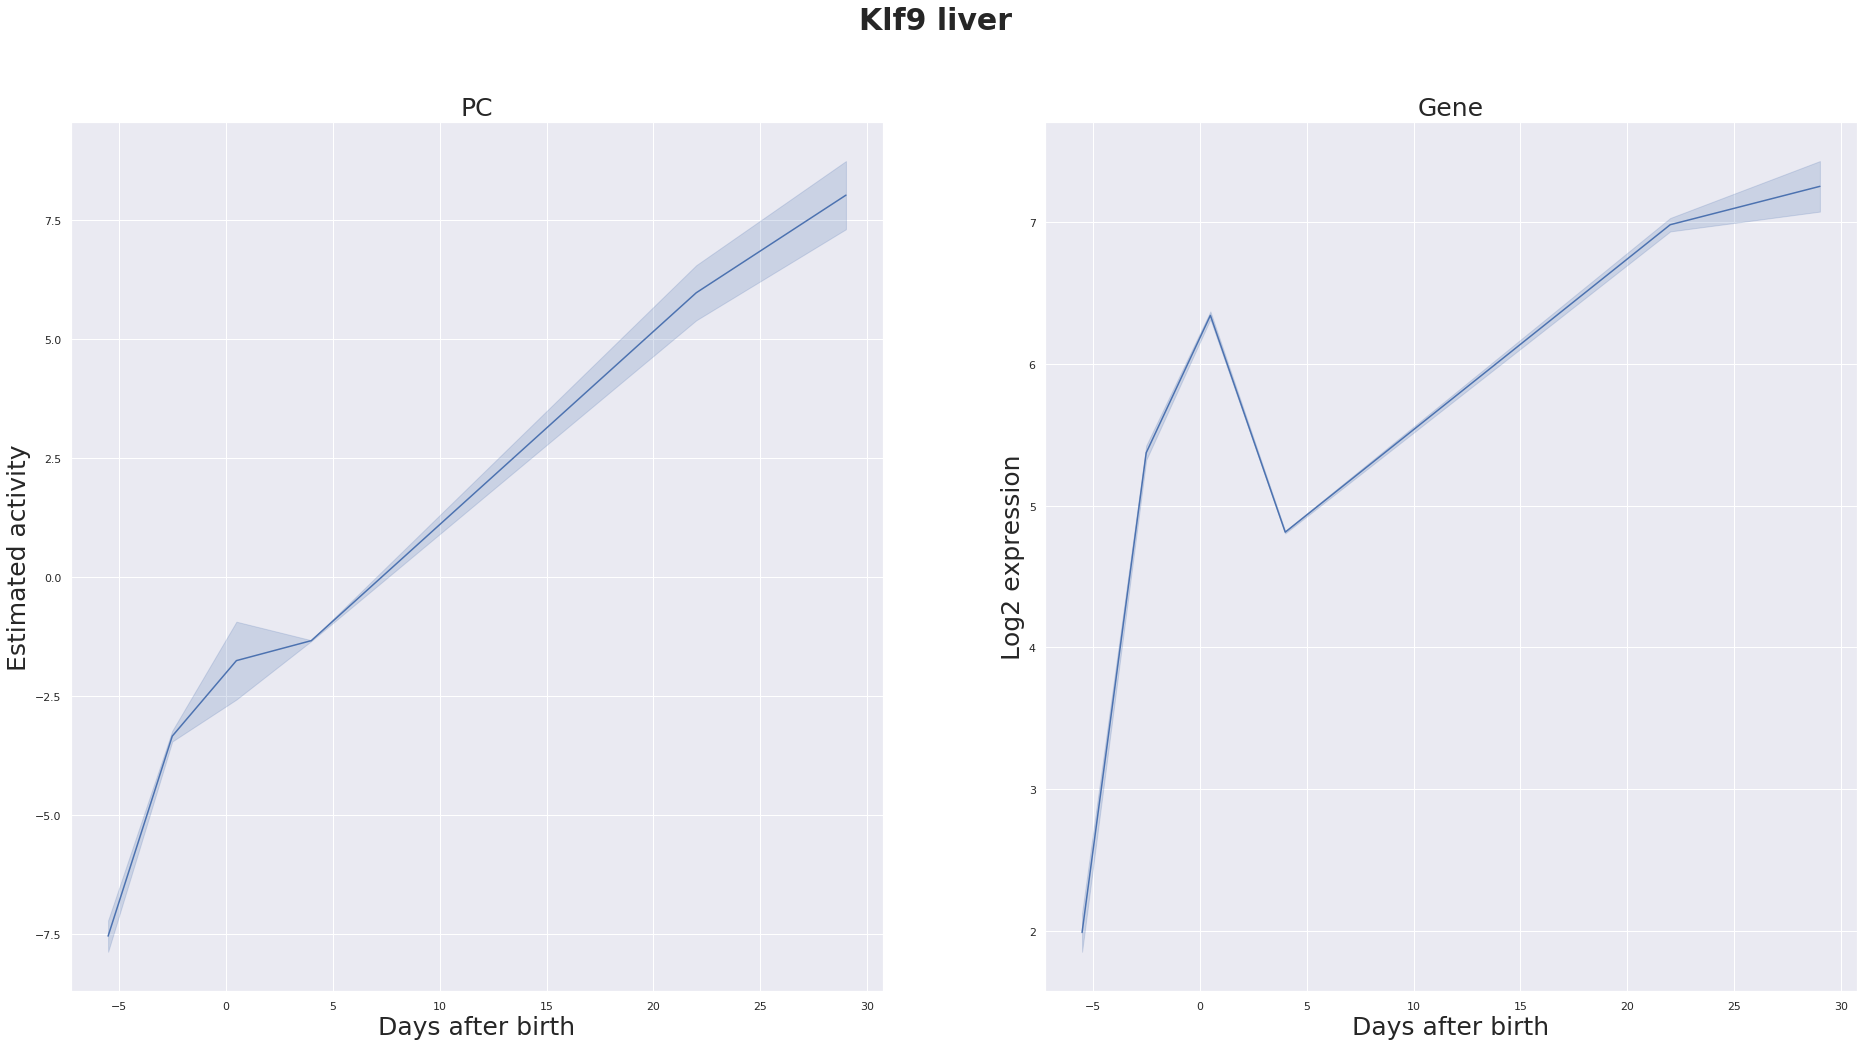
\includegraphics[width=6cm,height=3cm]{Figures&amp;Cover/Activity_Klf9_liver_NonePCremoved_filtering_False.png}
    \vspace{0.25cm}
    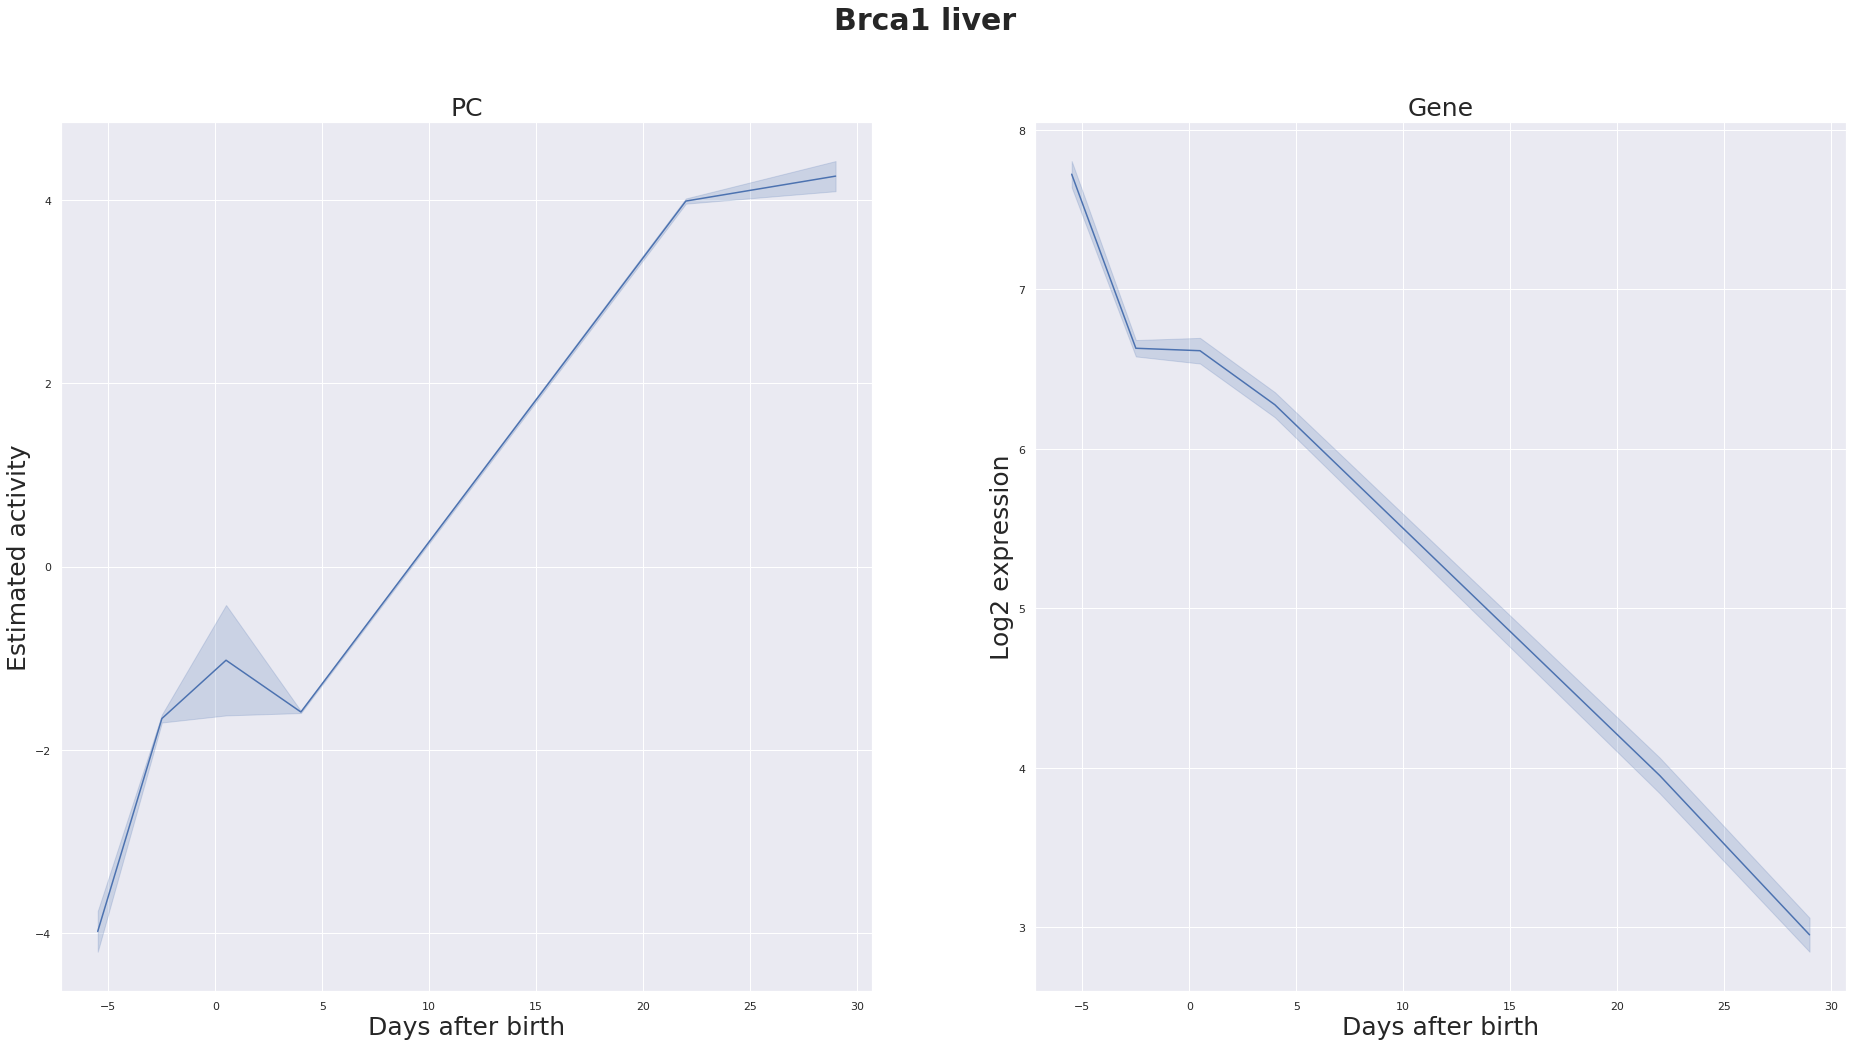
\includegraphics[width=6cm,height=3cm]{Figures&amp;Cover/Activity_Brca1_liver_NonePCremoved_filtering_False.png}
    \hspace{0.25cm}
    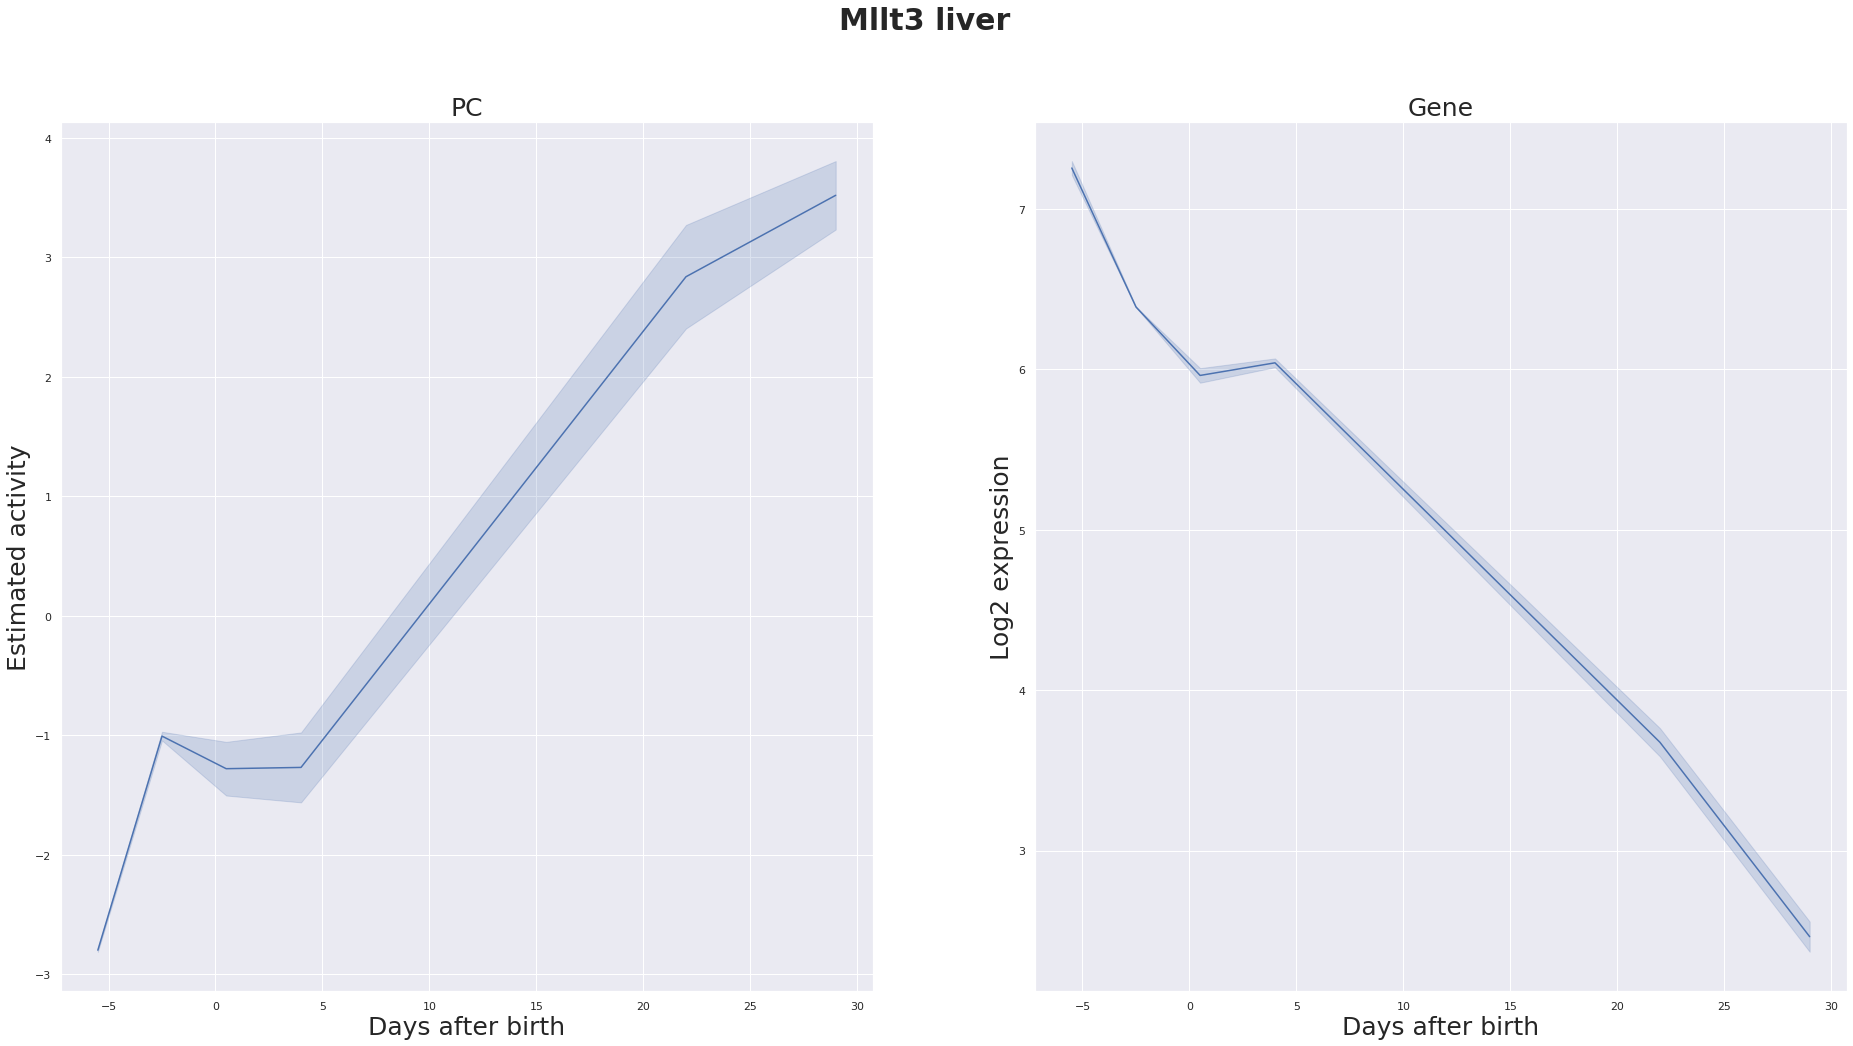
\includegraphics[width=6cm,height=3cm]{Figures&amp;Cover/Activity_Mllt3_liver_NonePCremoved_filtering_False.png}
    \vspace{0.25cm}
    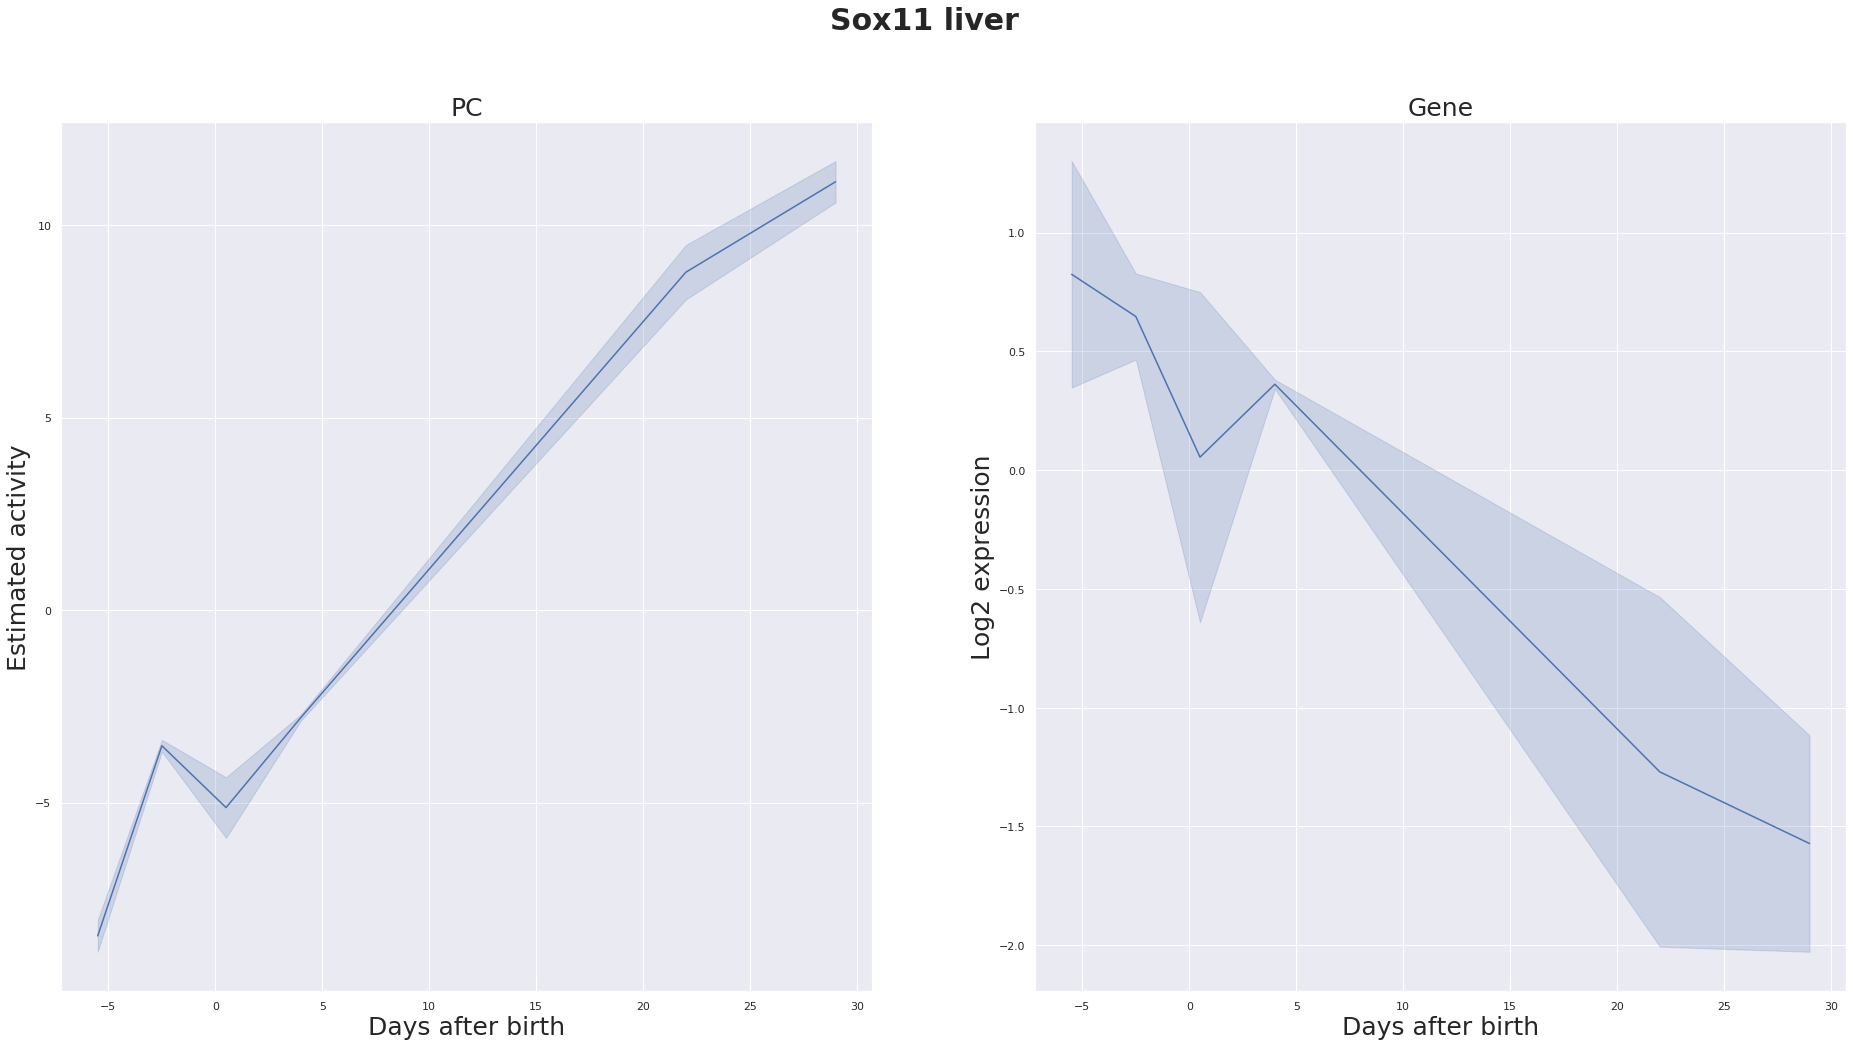
\includegraphics[width=6cm,height=3cm]{Figures&amp;Cover/Activity_Sox11_liver_NonePCremoved_filtering_False.png}
    \caption{\textbf{Estimated activities of Tal1, Lmo2, Ncapg, Ikzf1, Top2a, Klf9, Brca1, Mllt3 and Sox11 in mouse liver as a functions of the mices' age.} The activities were estimated by the first \ac{PC} of the mRNA expression data of the genes each \ac{TF} is likely to regulate (left figure of each pair) as well as directly through the transcription of the genes coding for each \ac{TF}, as log2-transformed \ac{RPM} transcript counts (right figure of each pair).}
    \label{fig:LiverEsts1}
\end{figure}

\begin{figure}
    \centering
    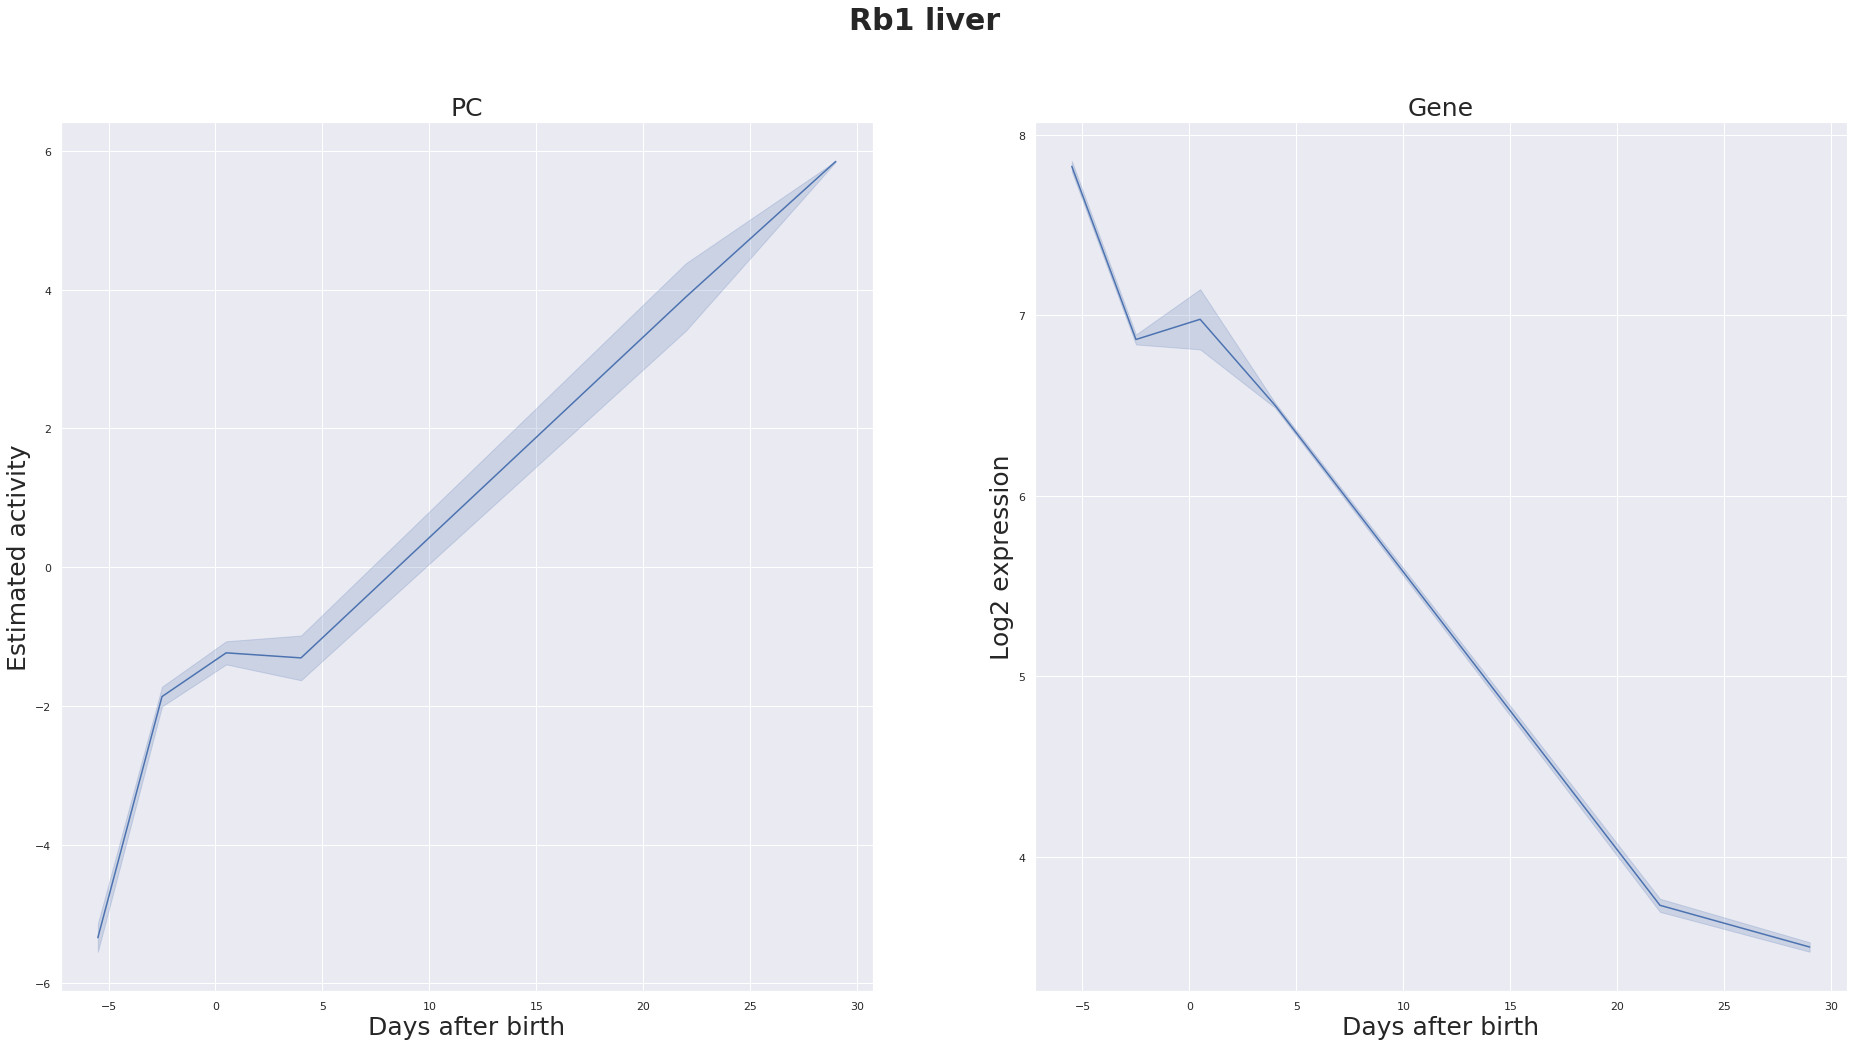
\includegraphics[width=6cm,height=3cm]{Figures&amp;Cover/Activity_Rb1_liver_NonePCremoved_filtering_False.png}
    \hspace{0.25cm}
    \vspace{0.25cm}
    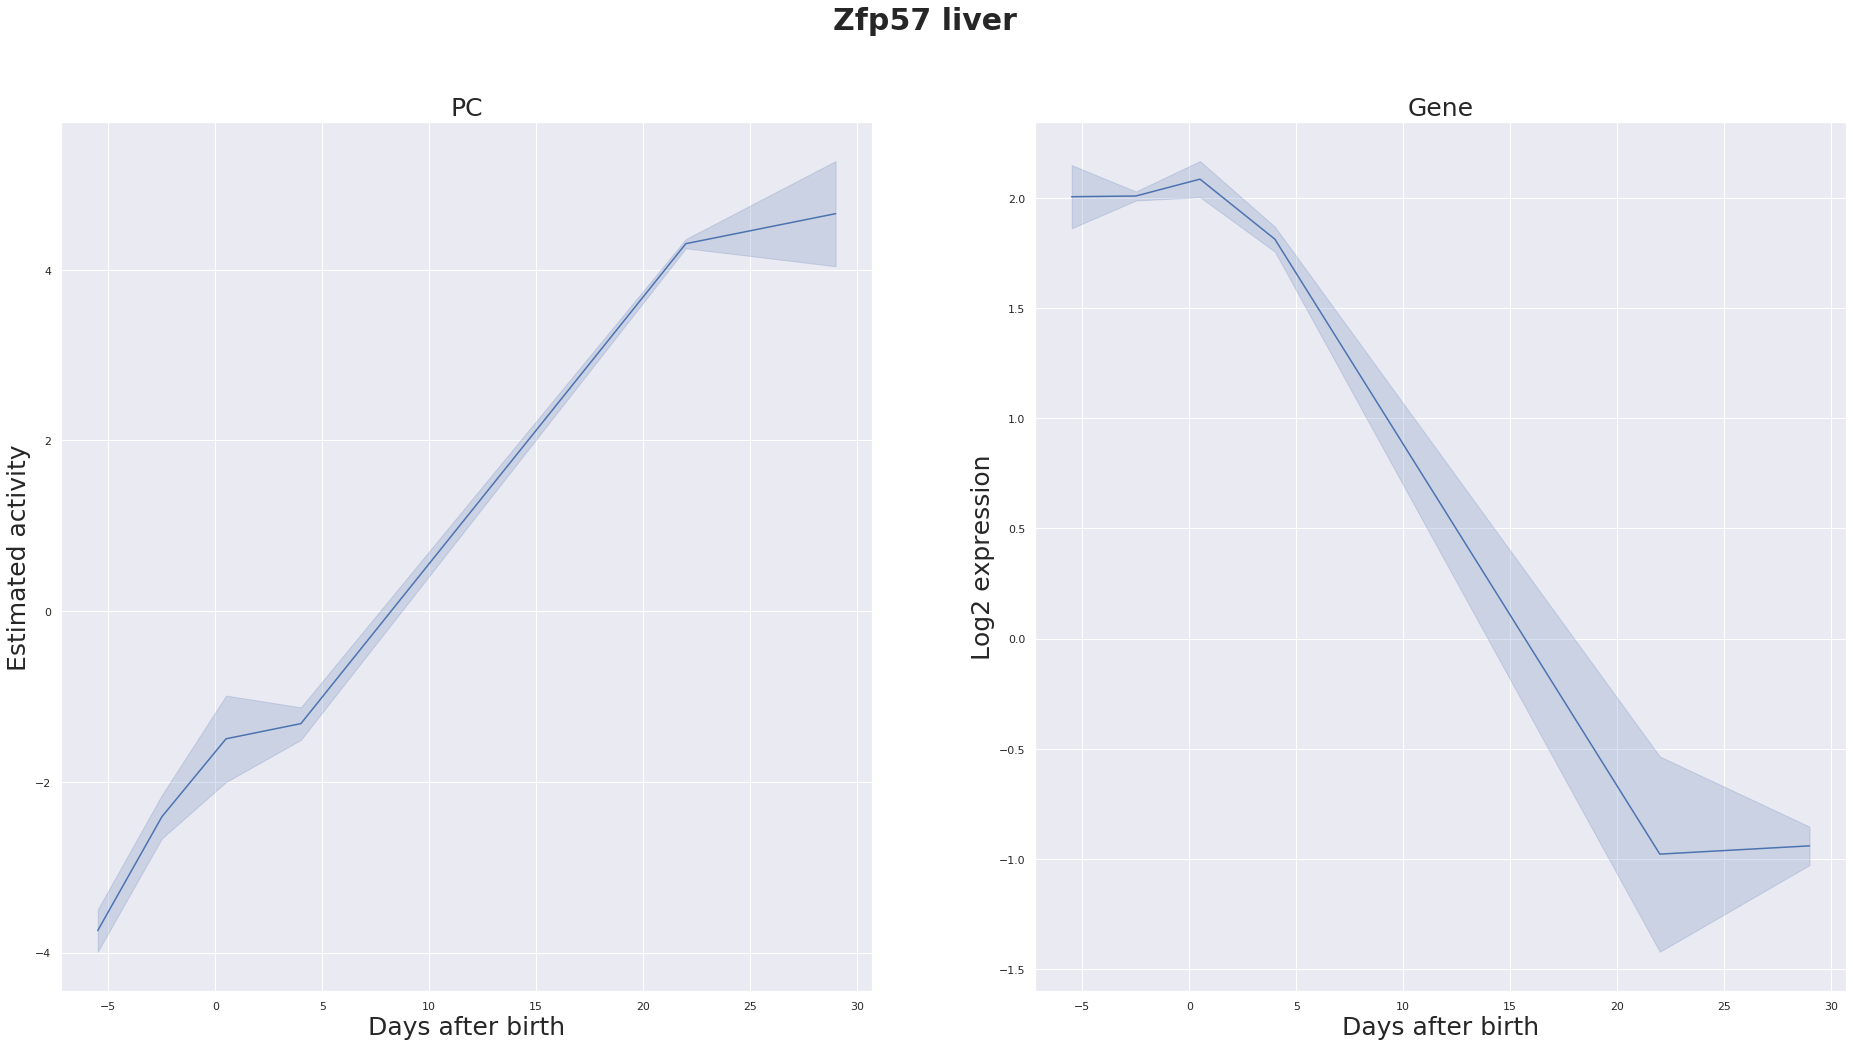
\includegraphics[width=6cm,height=3cm]{Figures&amp;Cover/Activity_Zfp57_liver_NonePCremoved_filtering_False.png}
    \vspace{0.25cm}
    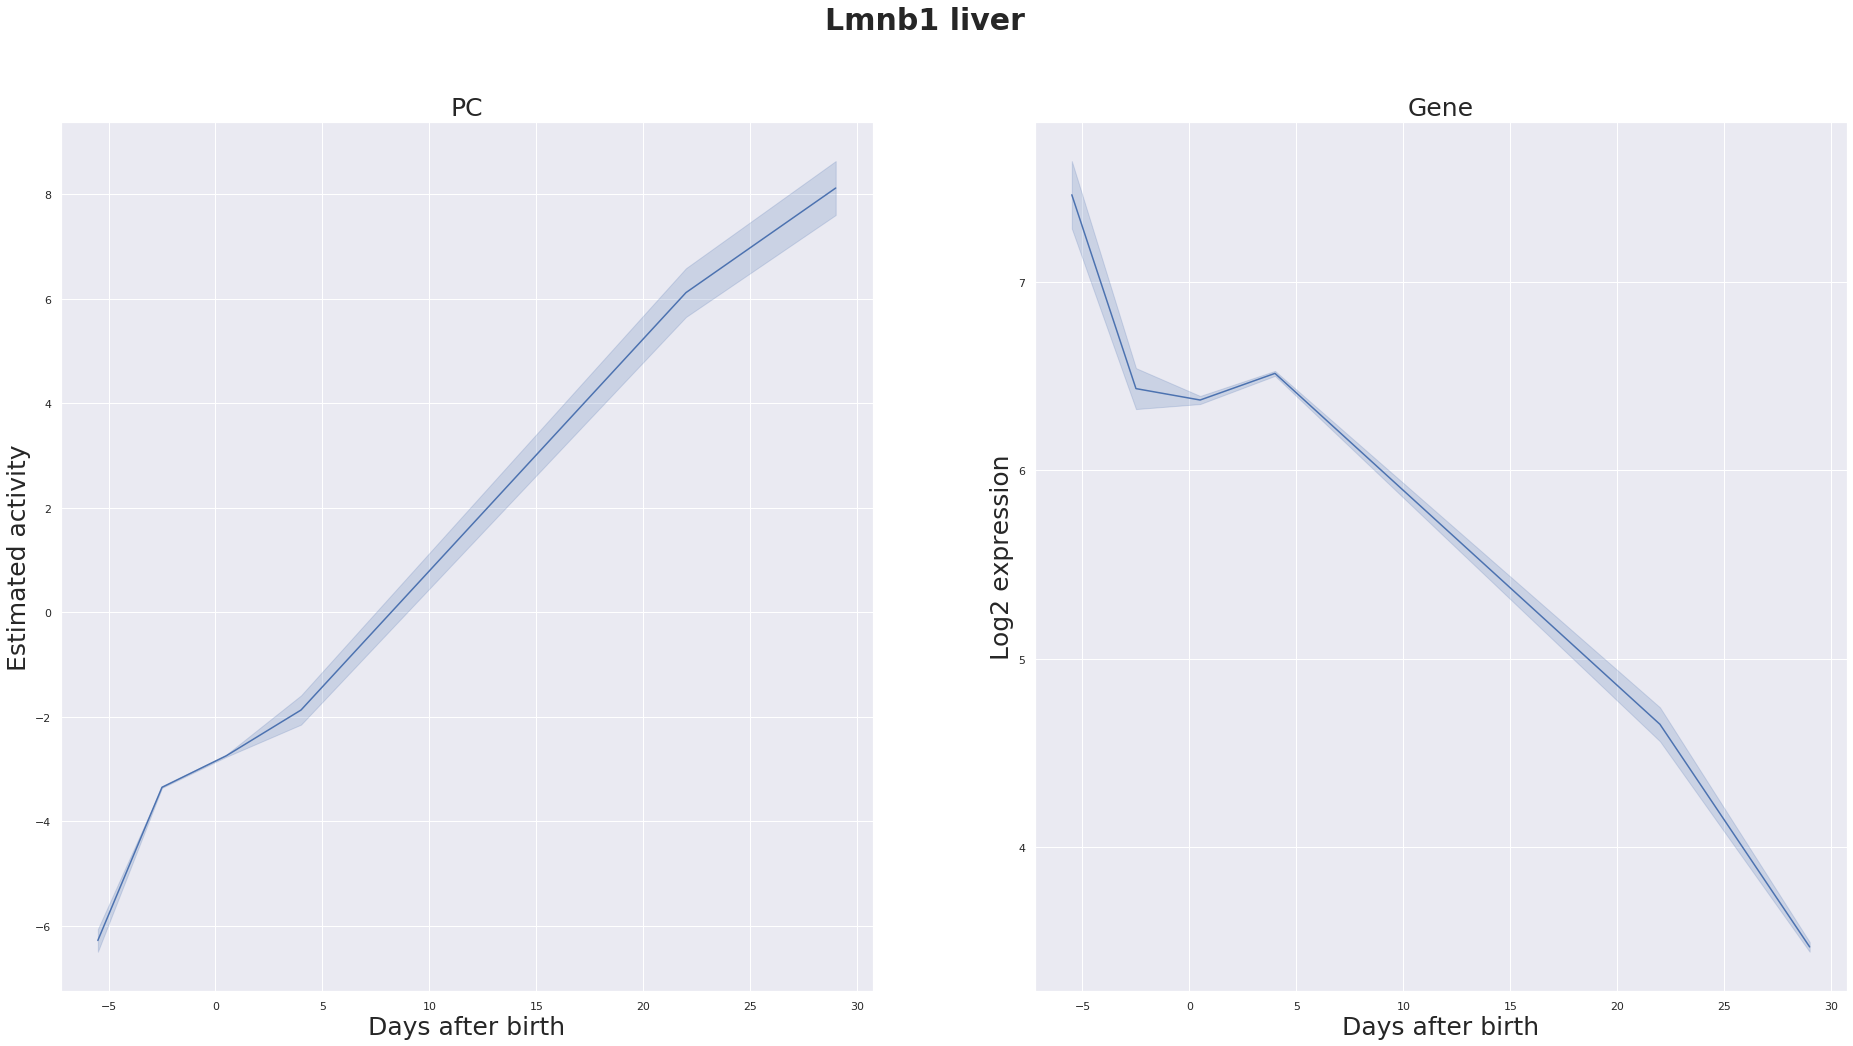
\includegraphics[width=6cm,height=3cm]{Figures&amp;Cover/Activity_Lmnb1_liver_NonePCremoved_filtering_False.png}
    \hspace{0.25cm}
    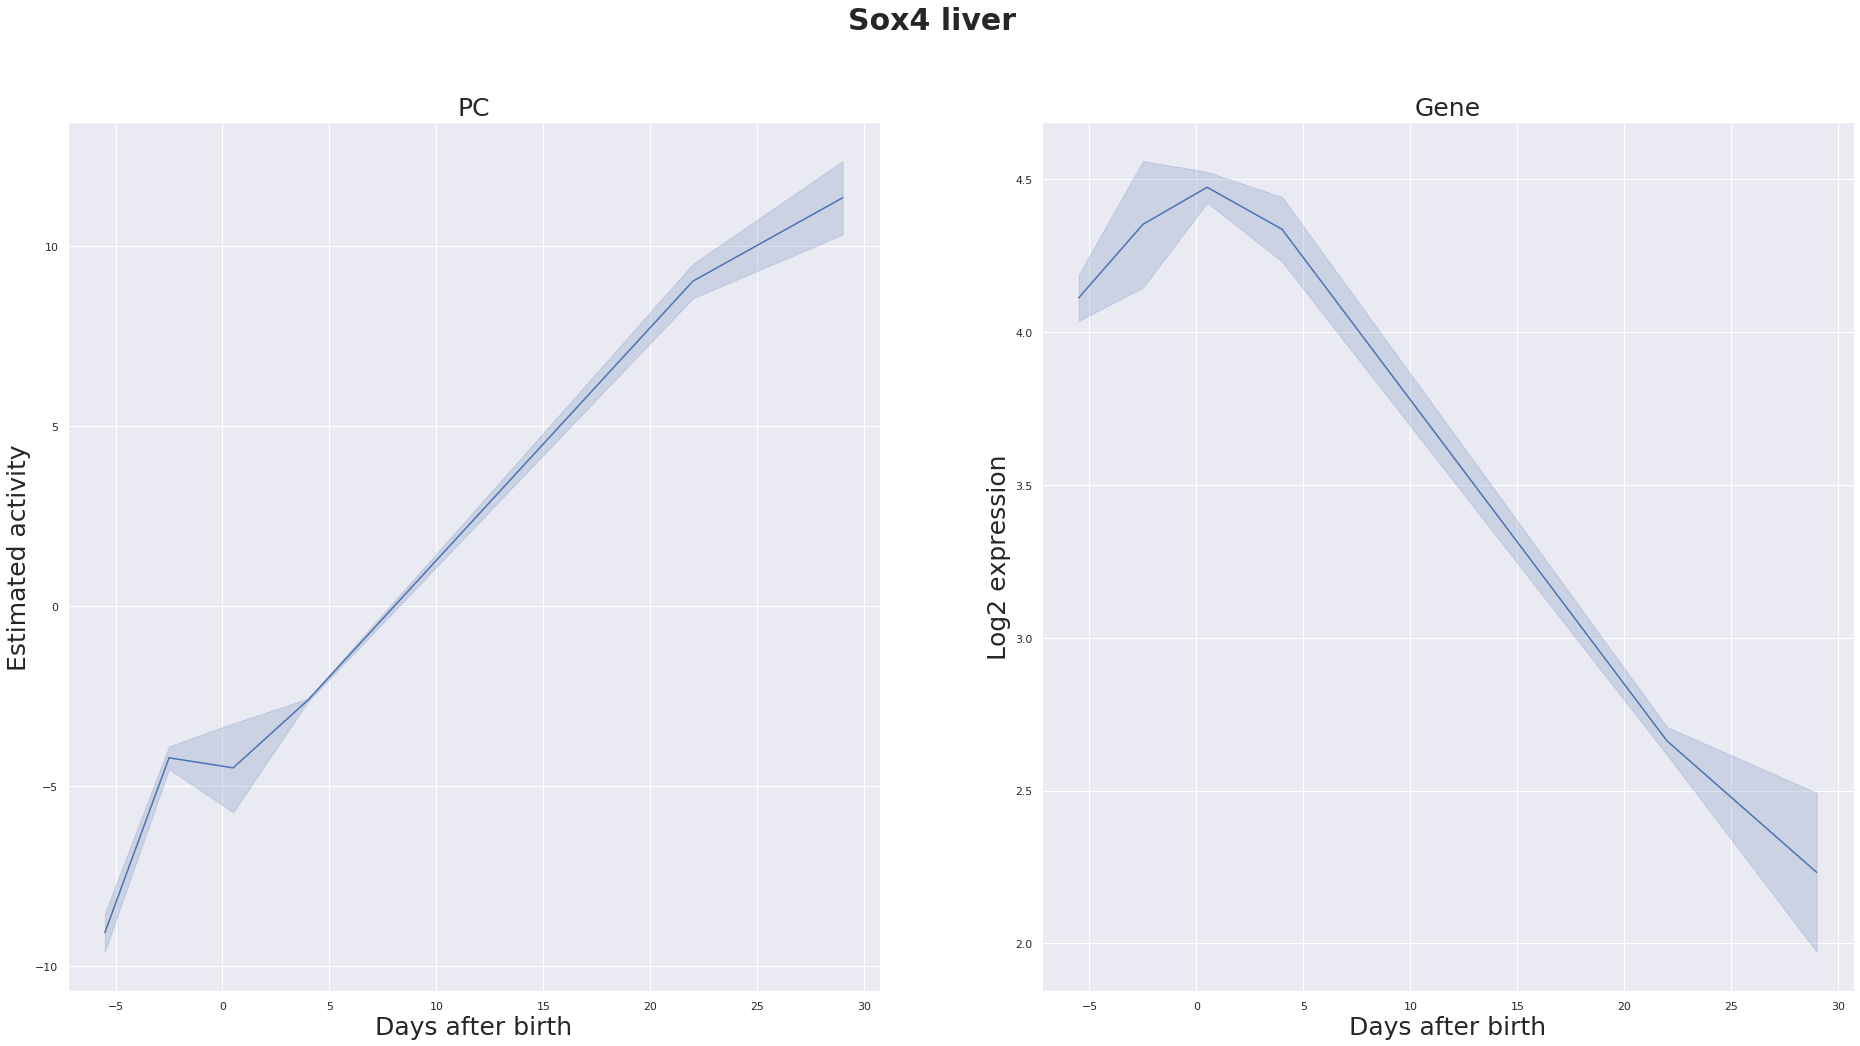
\includegraphics[width=6cm,height=3cm]{Figures&amp;Cover/Activity_Sox4_liver_NonePCremoved_filtering_False.png}
    \vspace{0.25cm}
    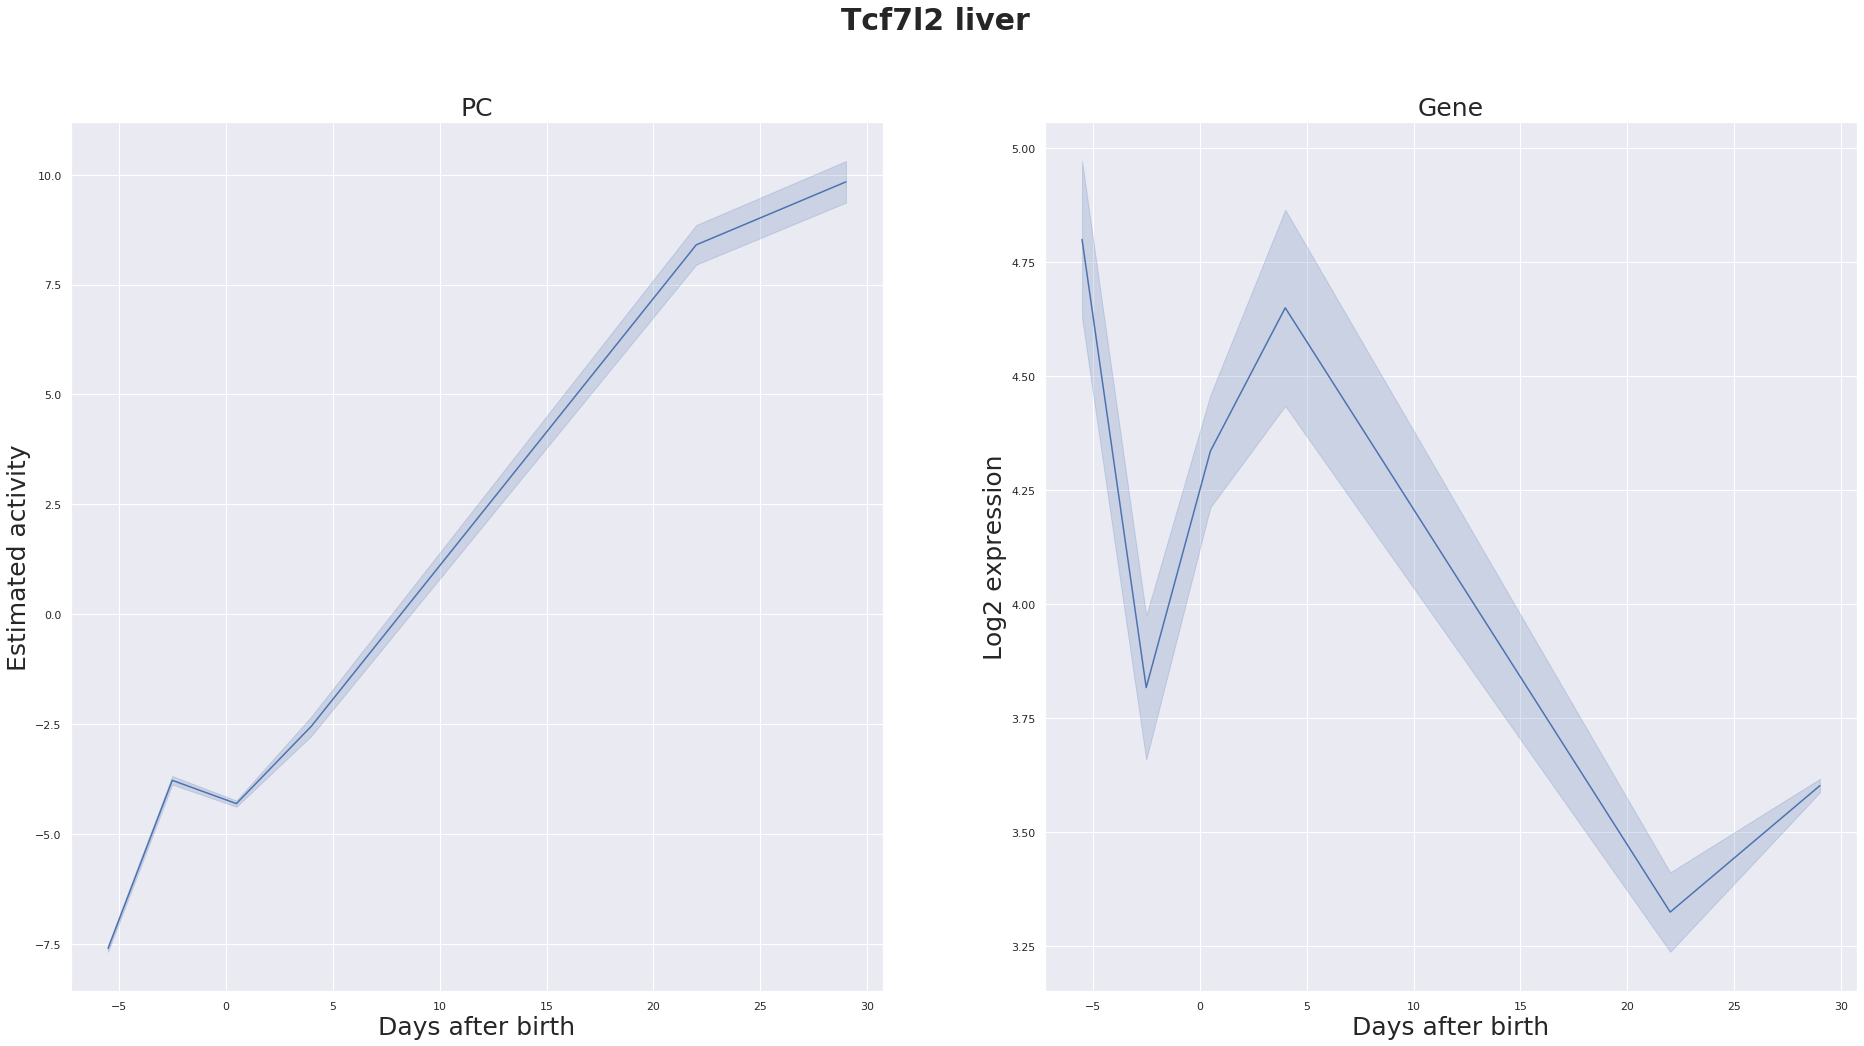
\includegraphics[width=6cm,height=3cm]{Figures&amp;Cover/Activity_Tcf7l2_liver_NonePCremoved_filtering_False.png}
    \hspace{0.25cm}
    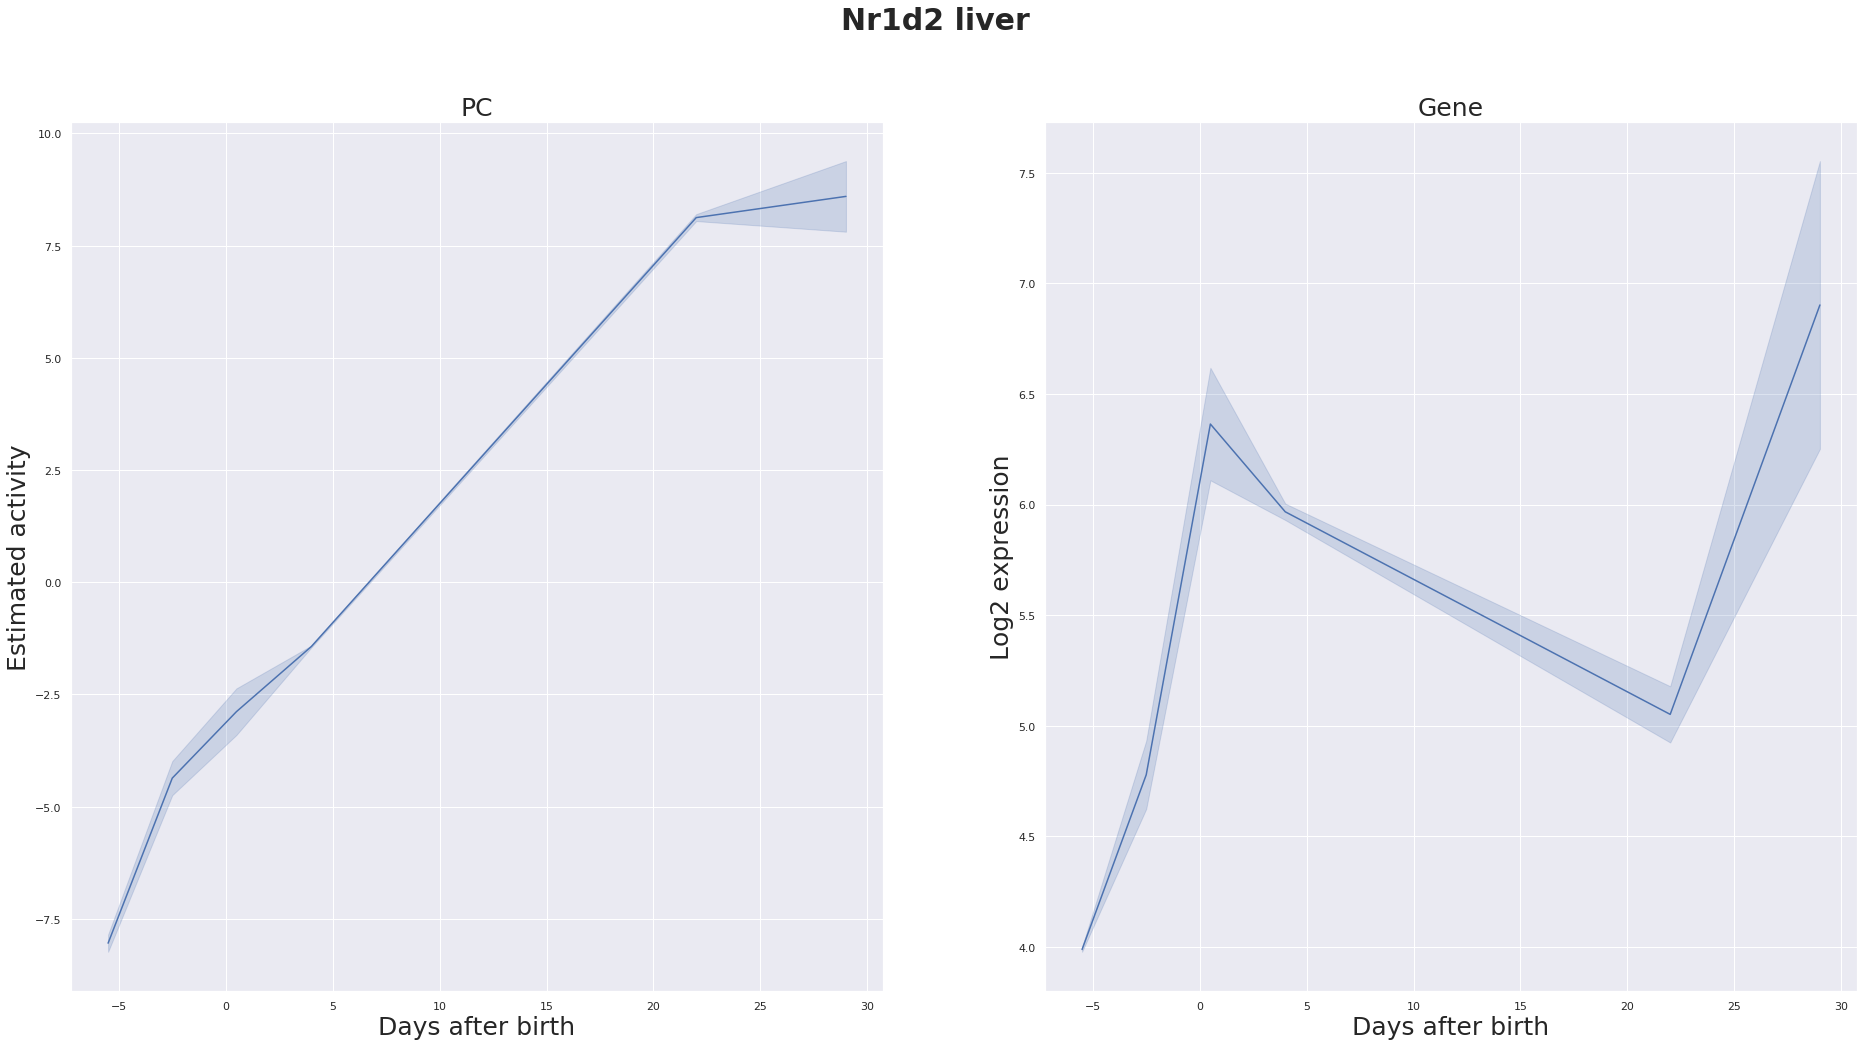
\includegraphics[width=6cm,height=3cm]{Figures&amp;Cover/Activity_Nr1d2_liver_NonePCremoved_filtering_False.png}
    \vspace{0.25cm}
    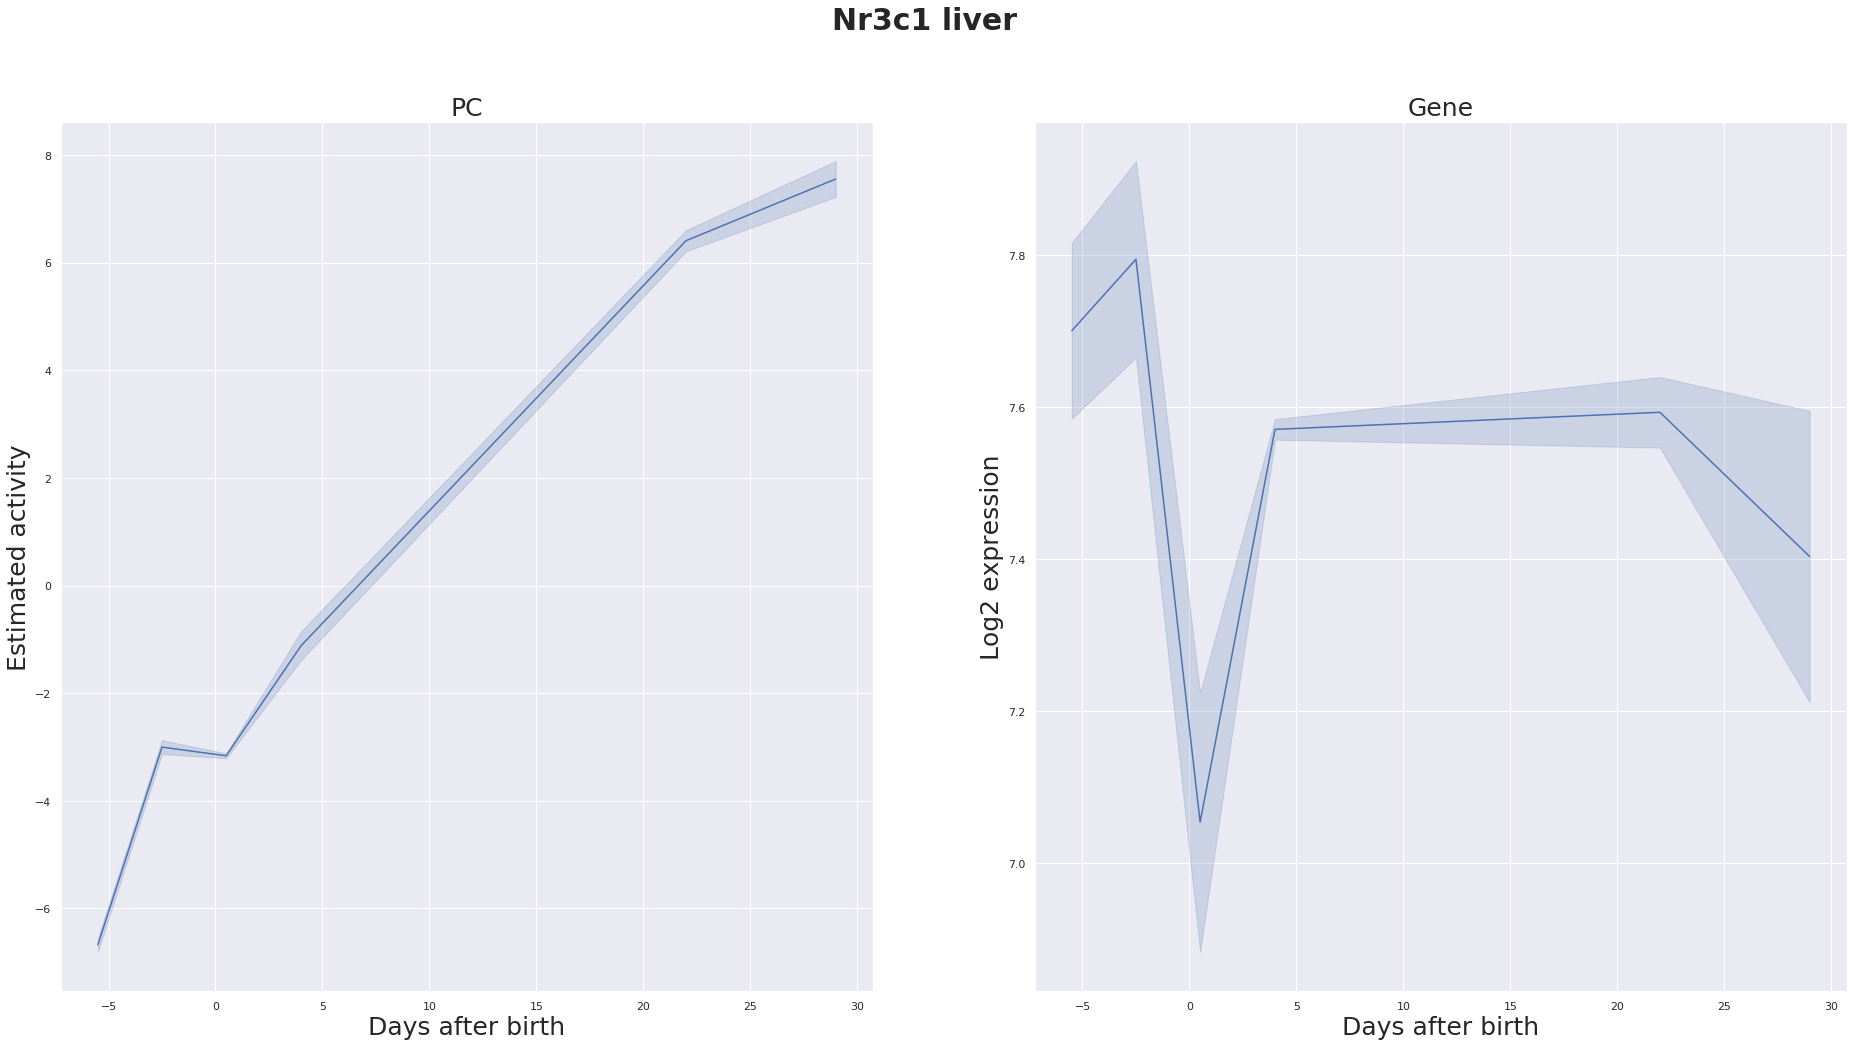
\includegraphics[width=6cm,height=3cm]{Figures&amp;Cover/Activity_Nr3c1_liver_NonePCremoved_filtering_False.png}
    \hspace{0.25cm}
    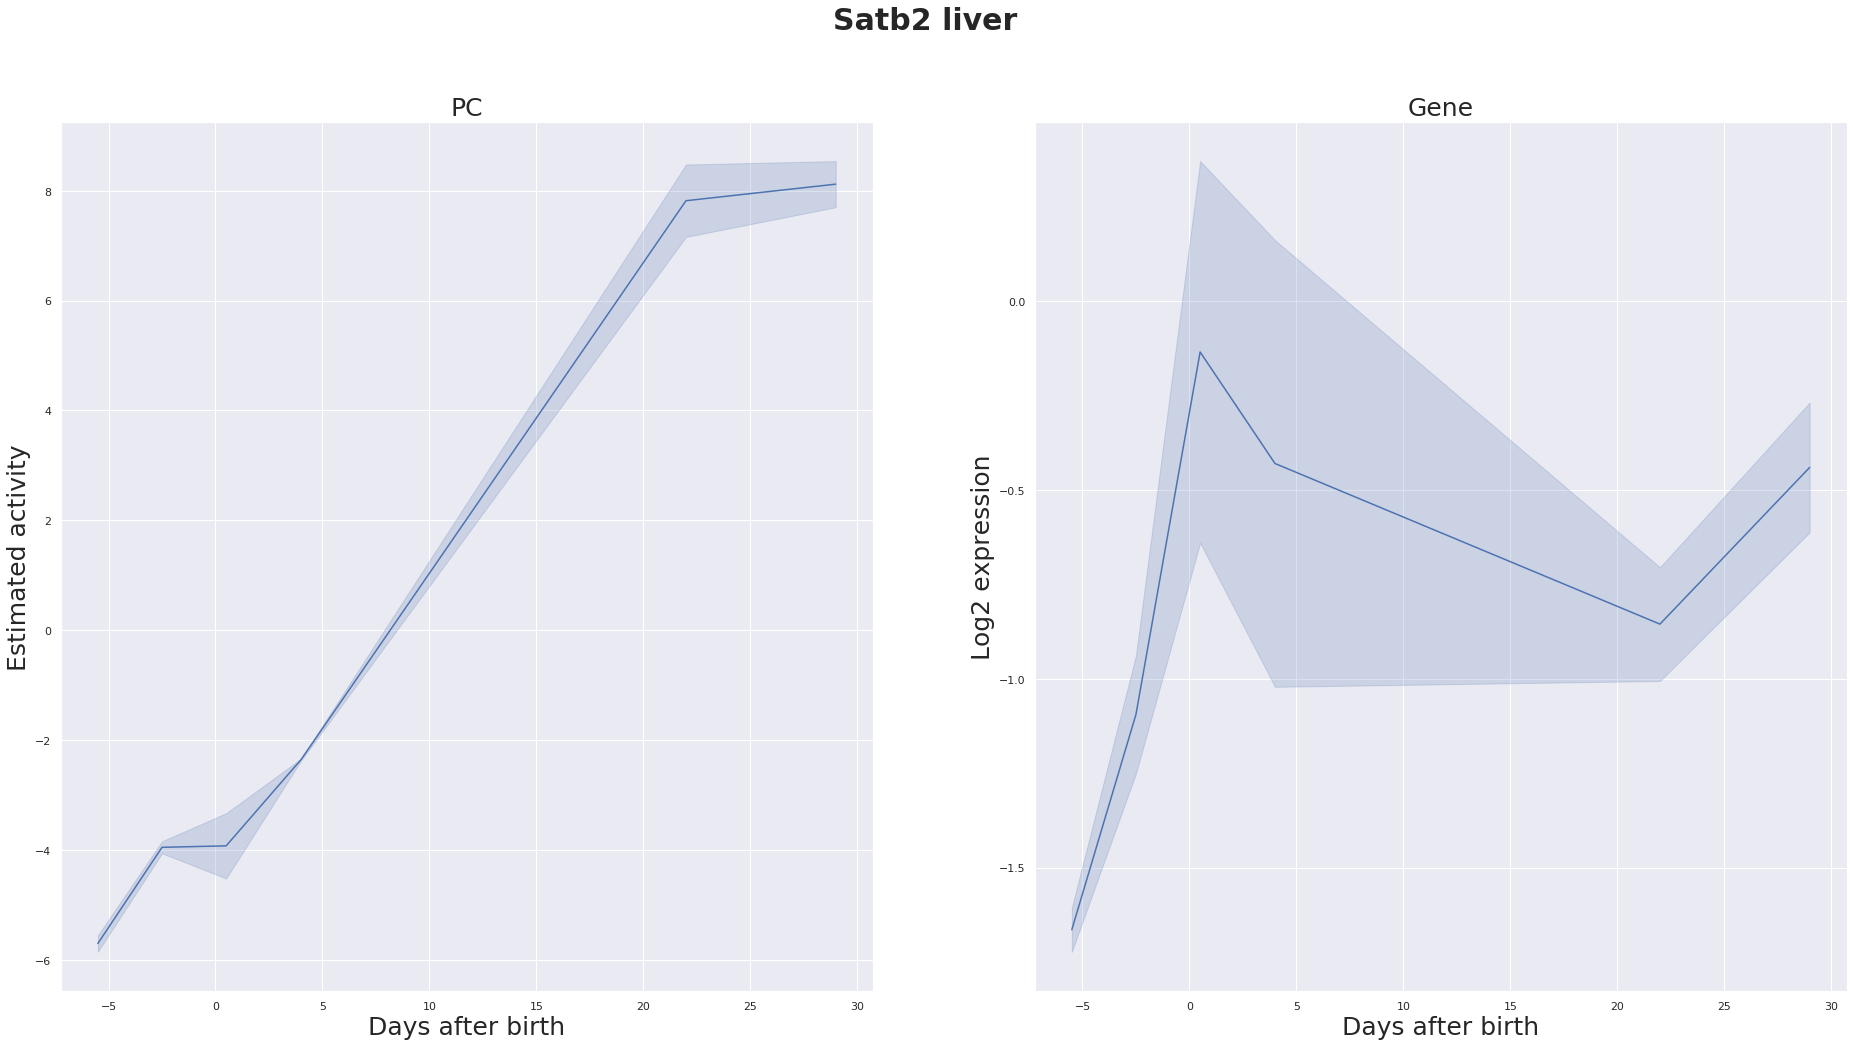
\includegraphics[width=6cm,height=3cm]{Figures&amp;Cover/Activity_Satb2_liver_NonePCremoved_filtering_False.png}
    \caption{\textbf{Estimated activities of Rb1, Zfp57, Lmnb1, Sox4, Tc7l2, Nr1d2, Nr3c1 and Satb2 in mouse liver as a functions of the mices' age.} The activities were estimated by the first \ac{PC} of the mRNA expression data of the genes each \ac{TF} is likely to regulate (left figure of each pair) as well as directly through the transcription of the genes coding for each \ac{TF}, as log2-transformed \ac{RPM} transcript counts (right figure of each pair).}
    \label{fig:LiverEsts2}
\end{figure}

% PC REMOVED

\begin{figure}
    \centering
    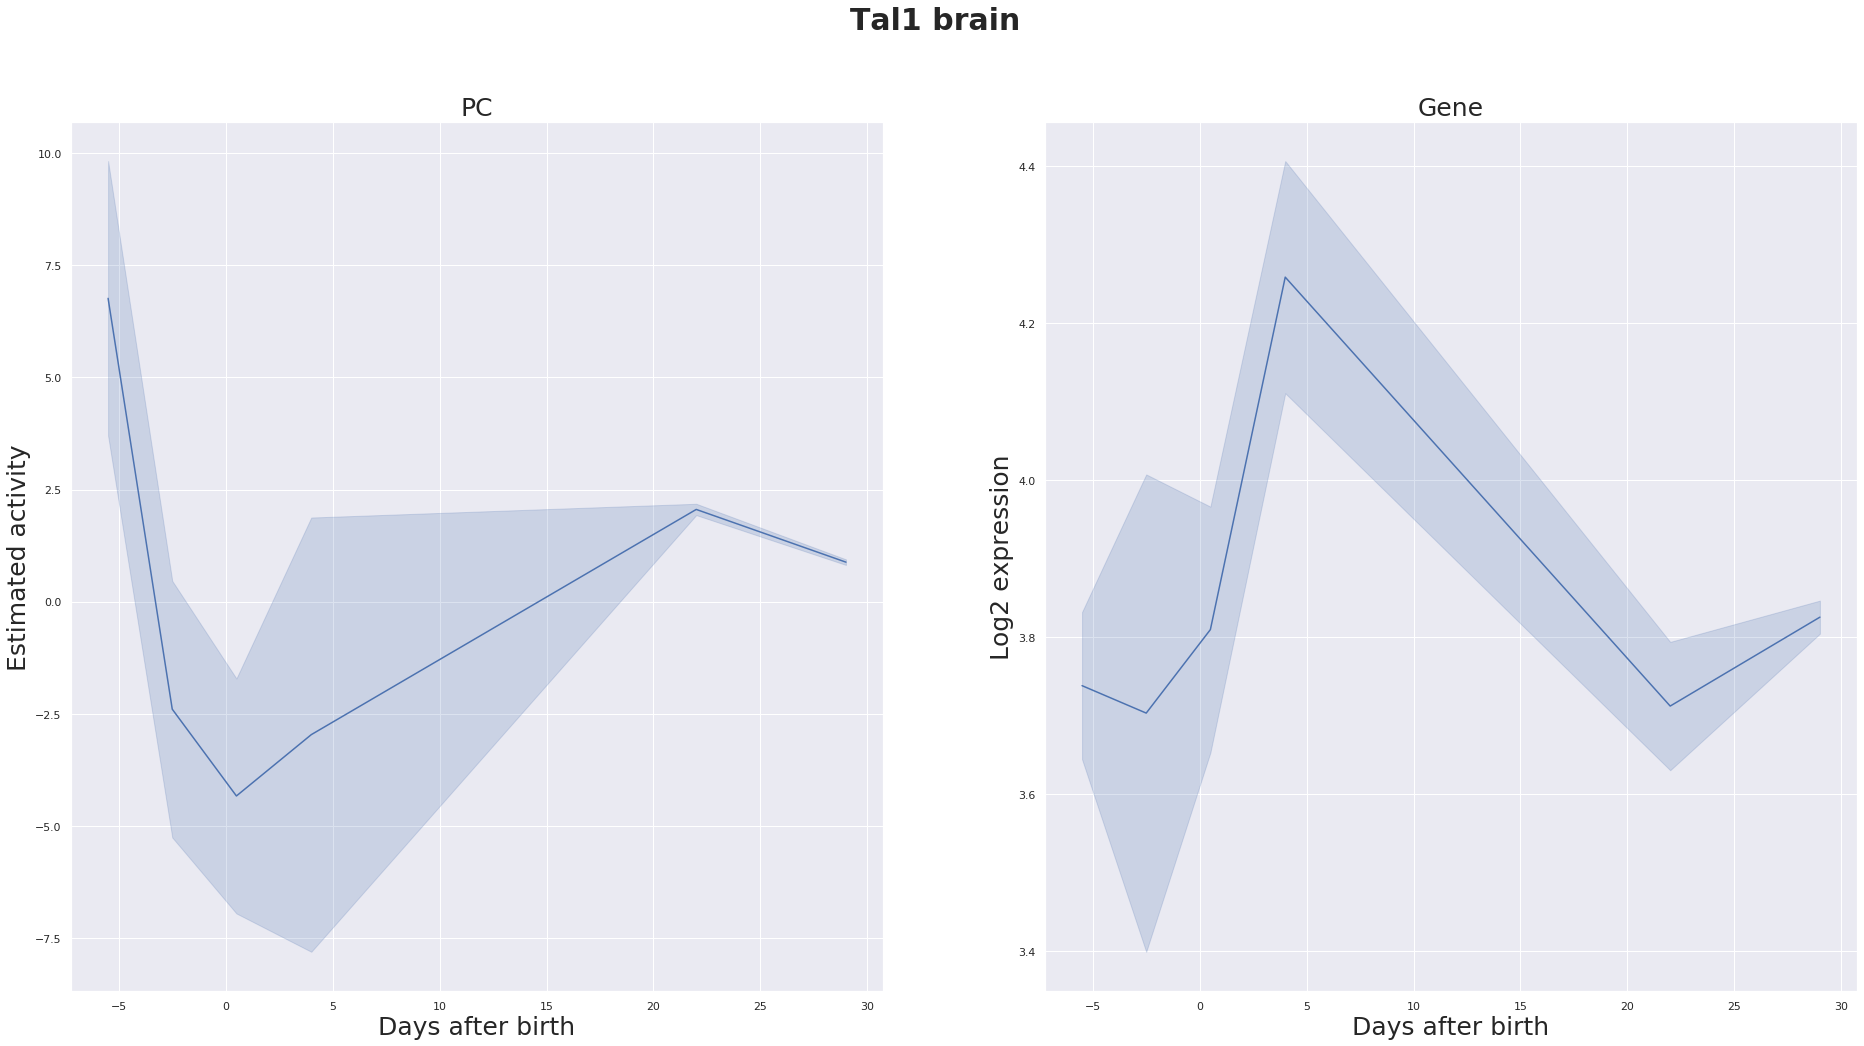
\includegraphics[width=6cm,height=3cm]{Figures&amp;Cover/Activity_Tal1_brain_1PCremoved_filtering_False.png}
    \hspace{0.25cm}
    \vspace{0.25cm}
    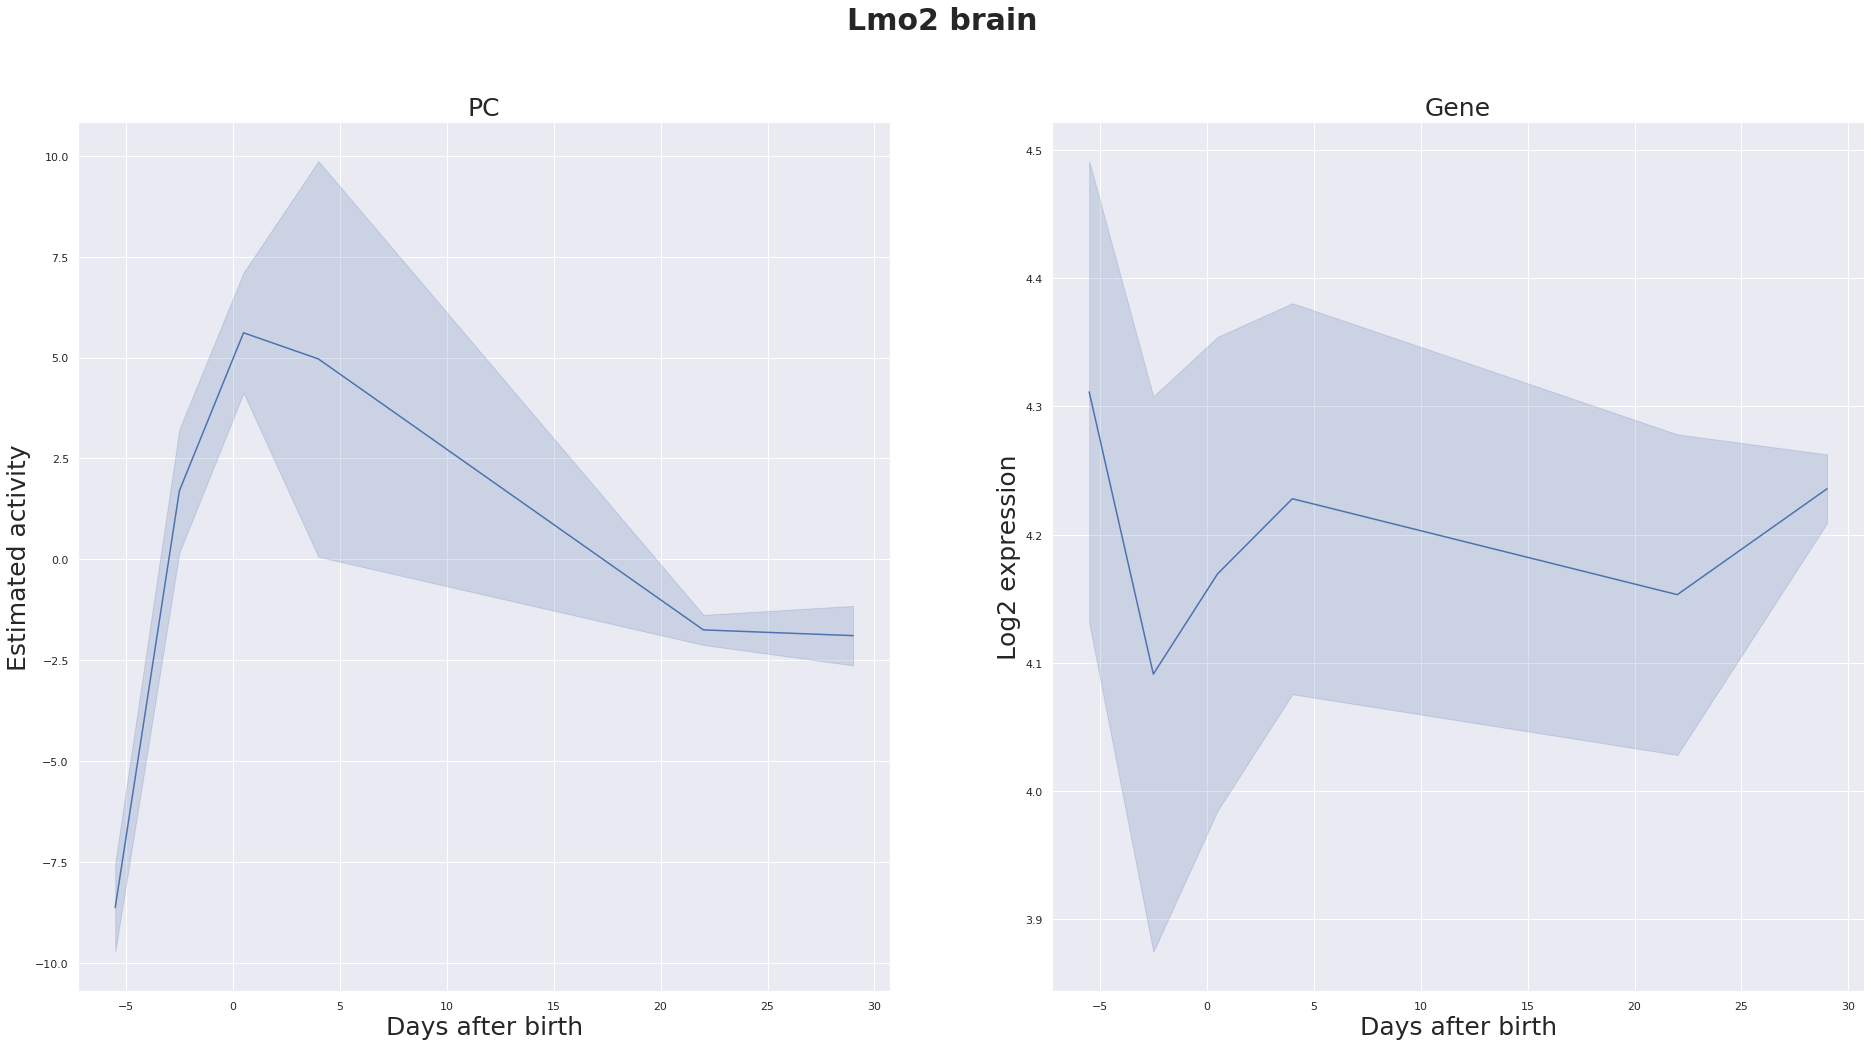
\includegraphics[width=6cm,height=3cm]{Figures&amp;Cover/Activity_Lmo2_brain_1PCremoved_filtering_False.png}
    \vspace{0.25cm}
    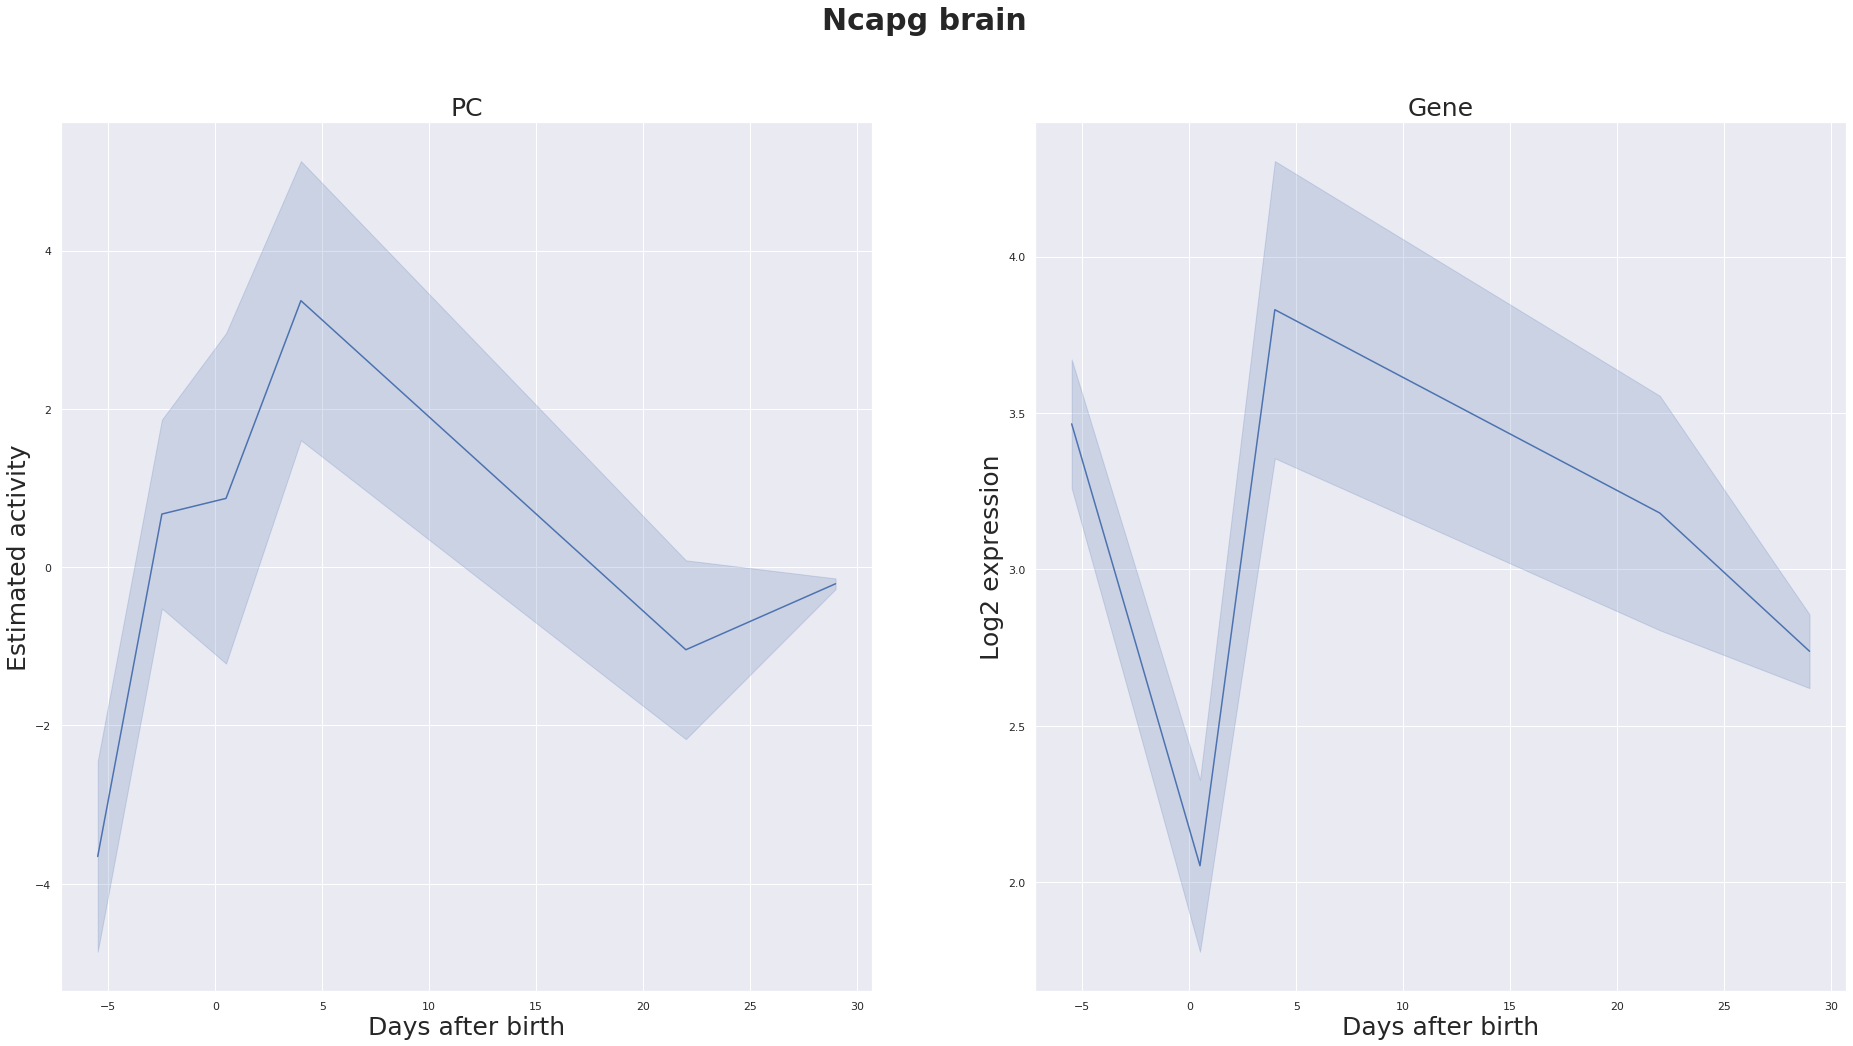
\includegraphics[width=6cm,height=3cm]{Figures&amp;Cover/Activity_Ncapg_brain_1PCremoved_filtering_False.png}
    \hspace{0.25cm}
    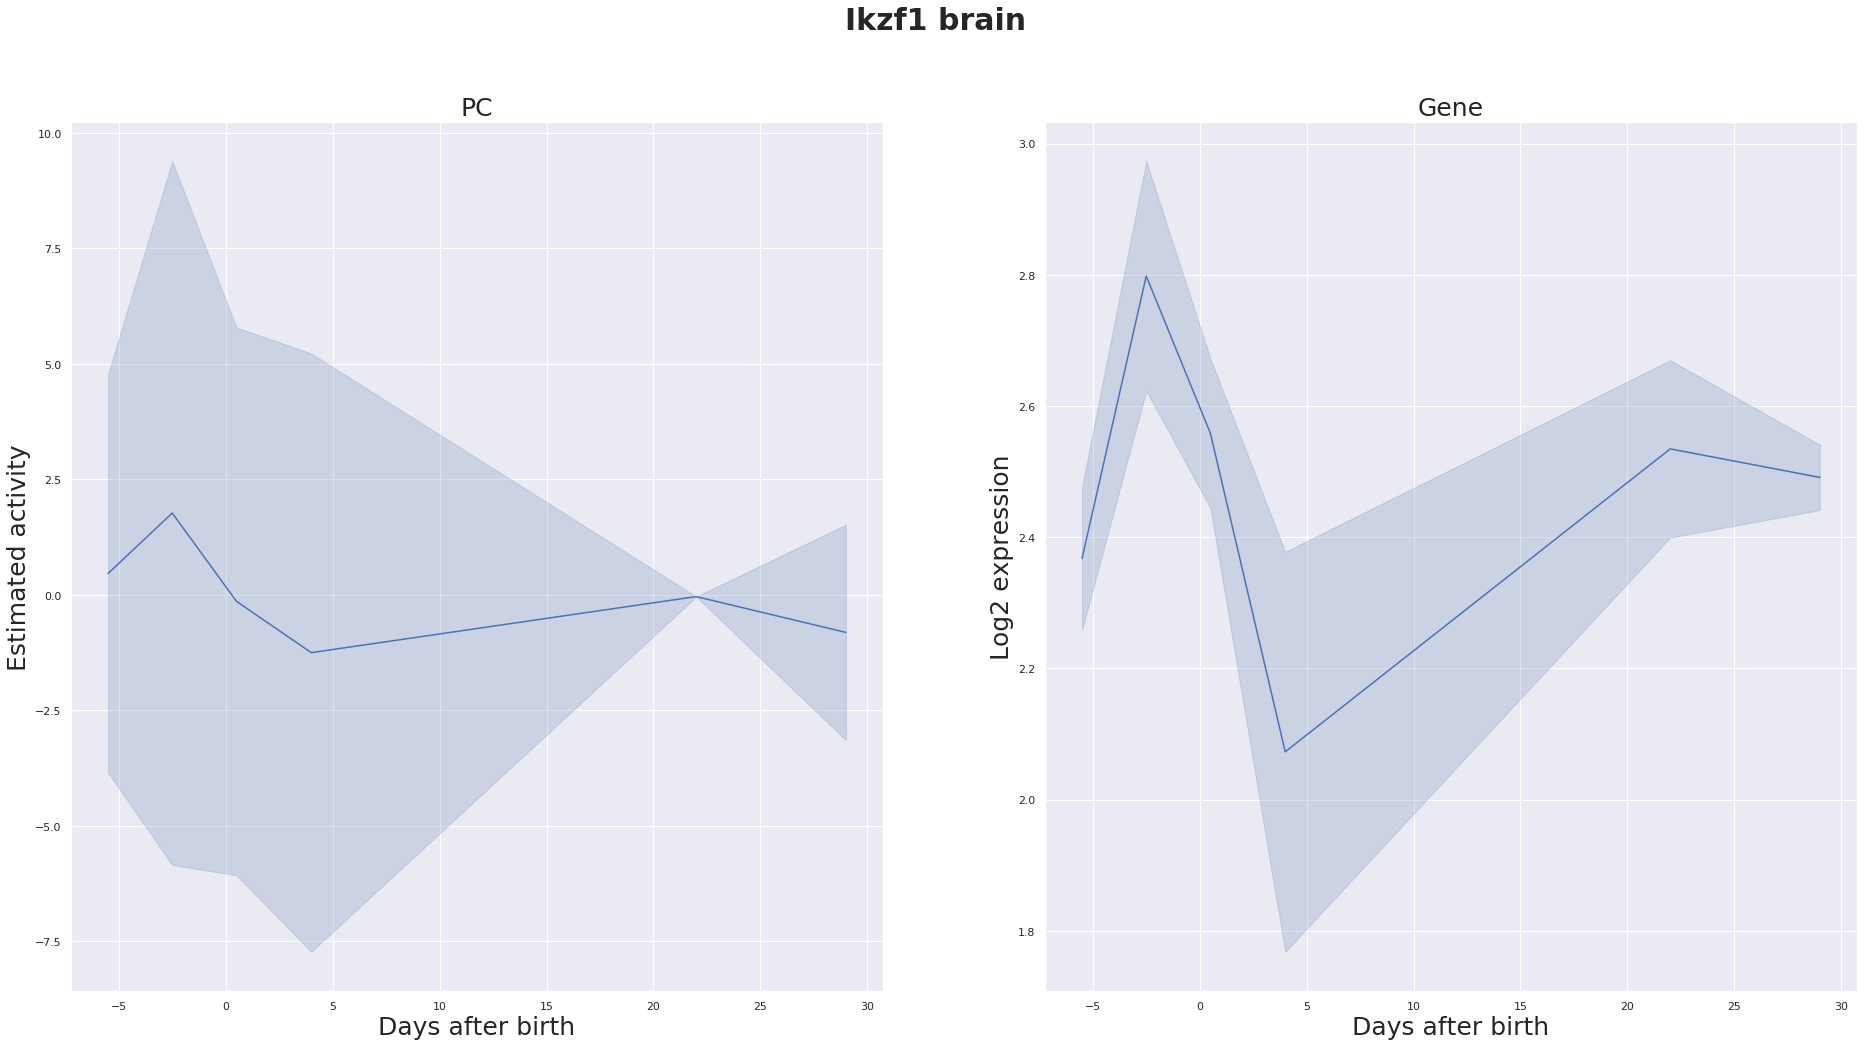
\includegraphics[width=6cm,height=3cm]{Figures&amp;Cover/Activity_Ikzf1_brain_1PCremoved_filtering_False.png}
    \vspace{0.25cm}
    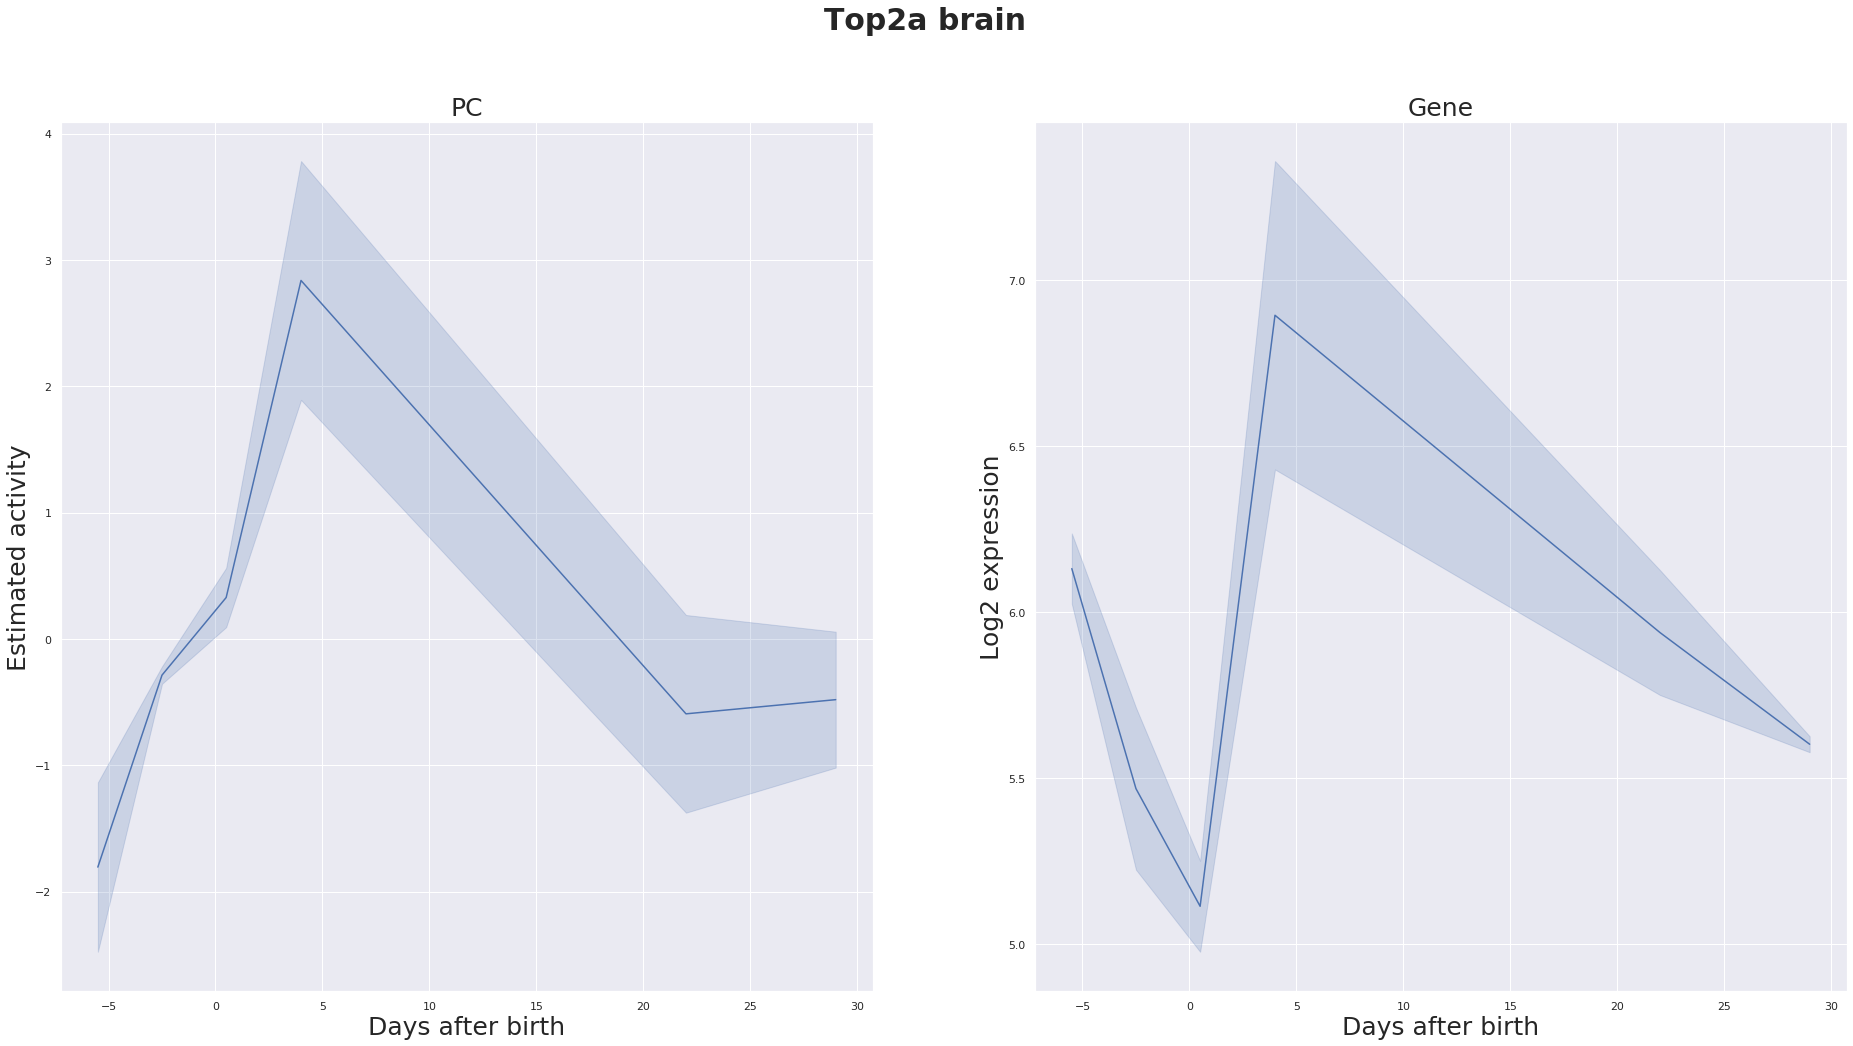
\includegraphics[width=6cm,height=3cm]{Figures&amp;Cover/Activity_Top2a_brain_1PCremoved_filtering_False.png}
    \hspace{0.25cm}
    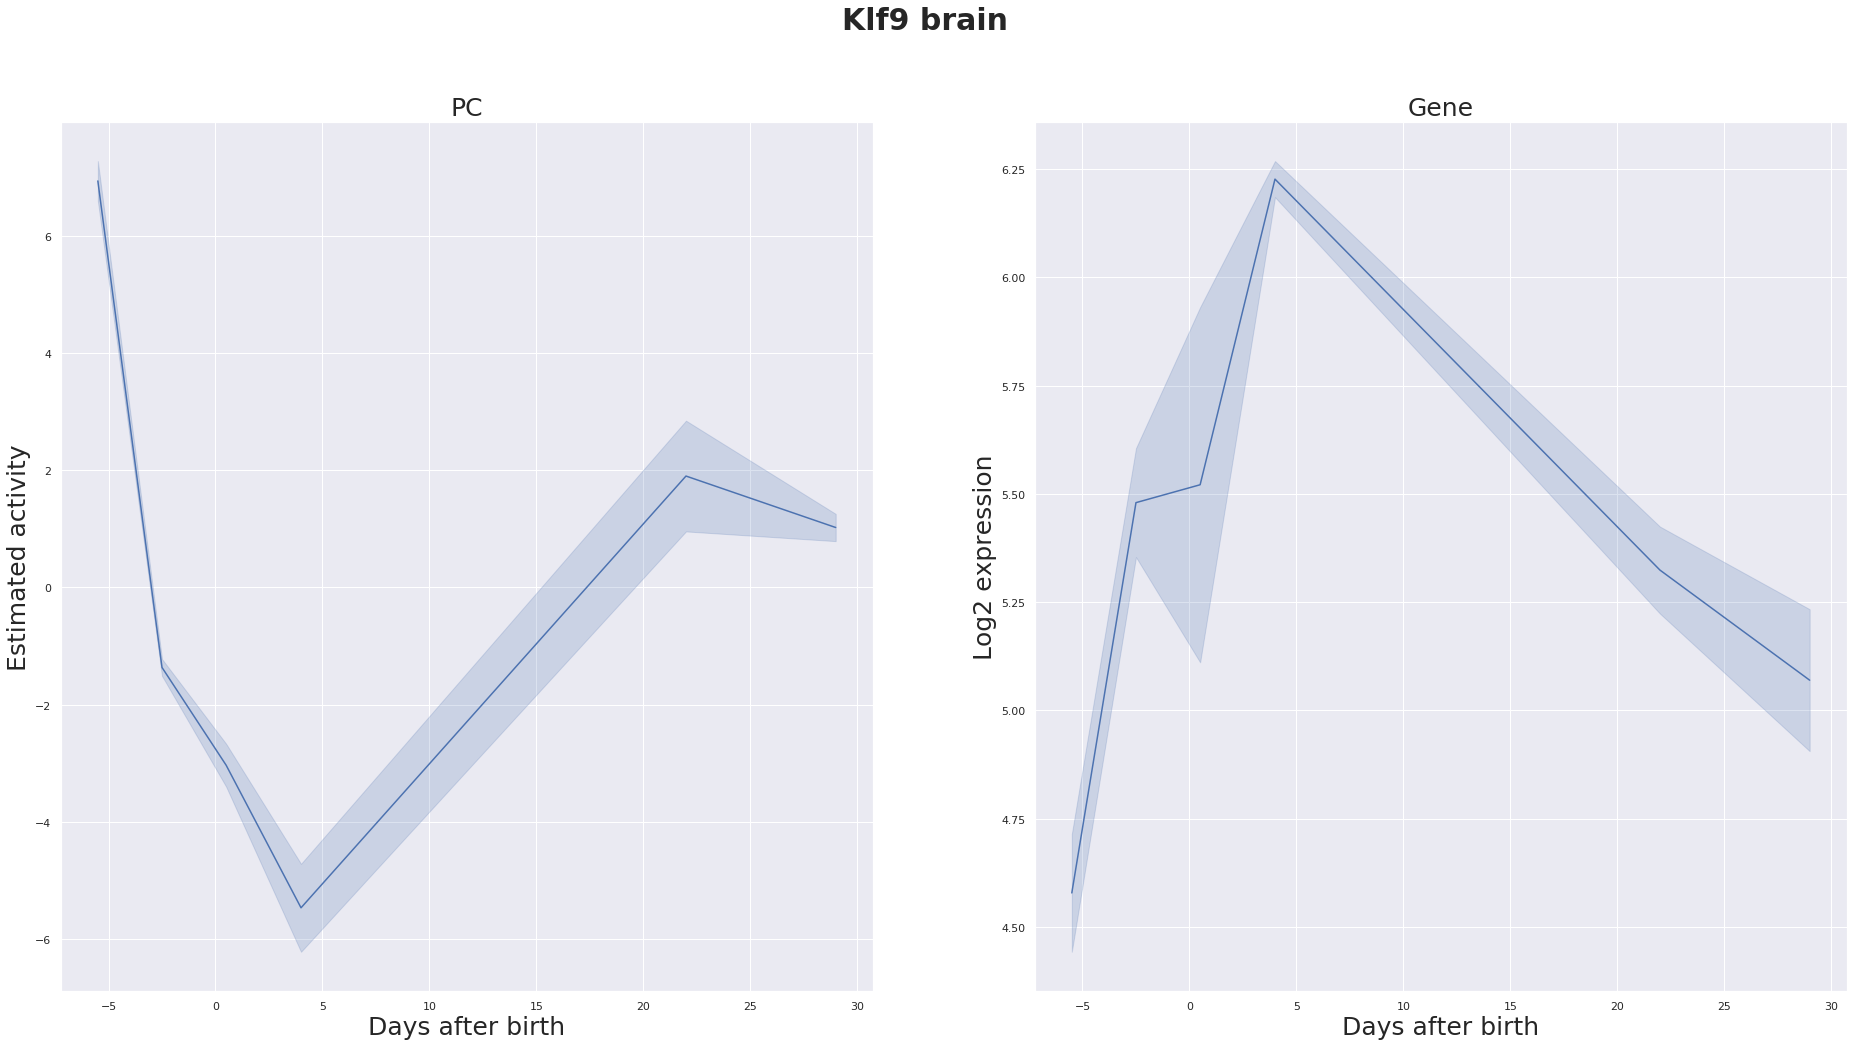
\includegraphics[width=6cm,height=3cm]{Figures&amp;Cover/Activity_Klf9_brain_1PCremoved_filtering_False.png}
    \vspace{0.25cm}
    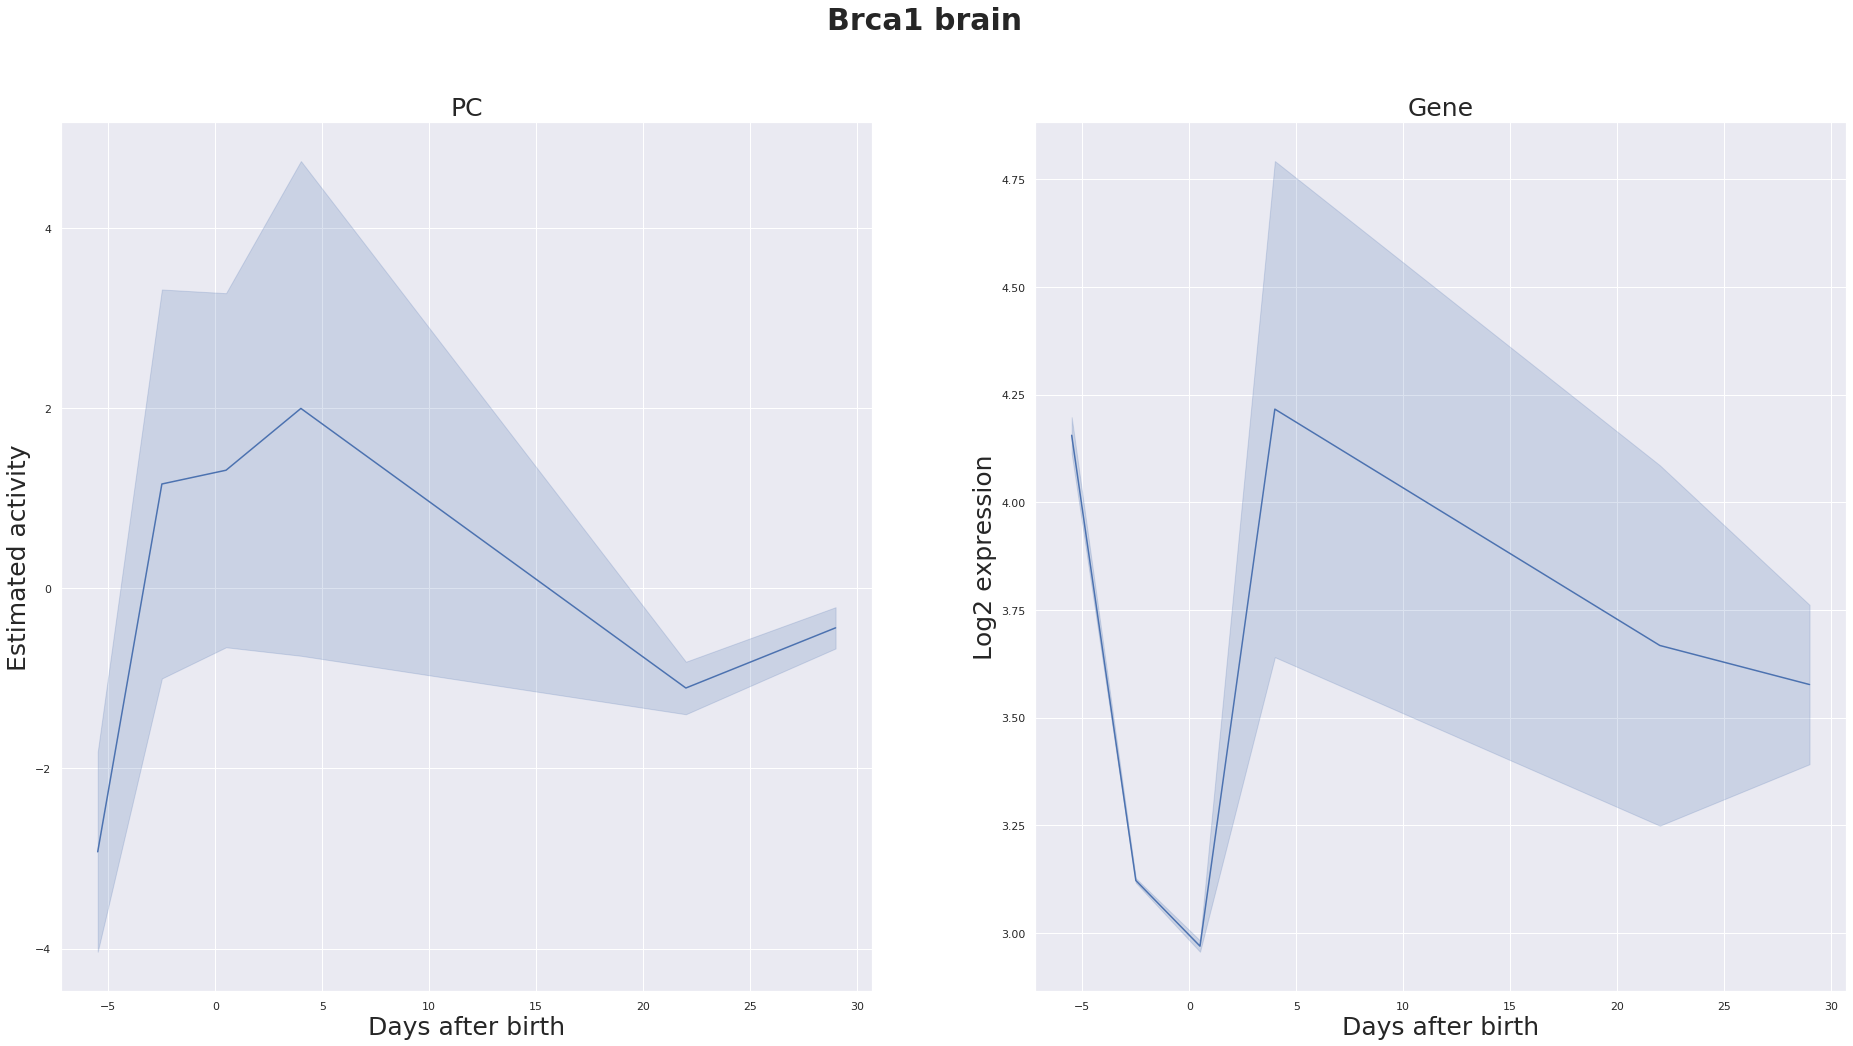
\includegraphics[width=6cm,height=3cm]{Figures&amp;Cover/Activity_Brca1_brain_1PCremoved_filtering_False.png}
    \hspace{0.25cm}
    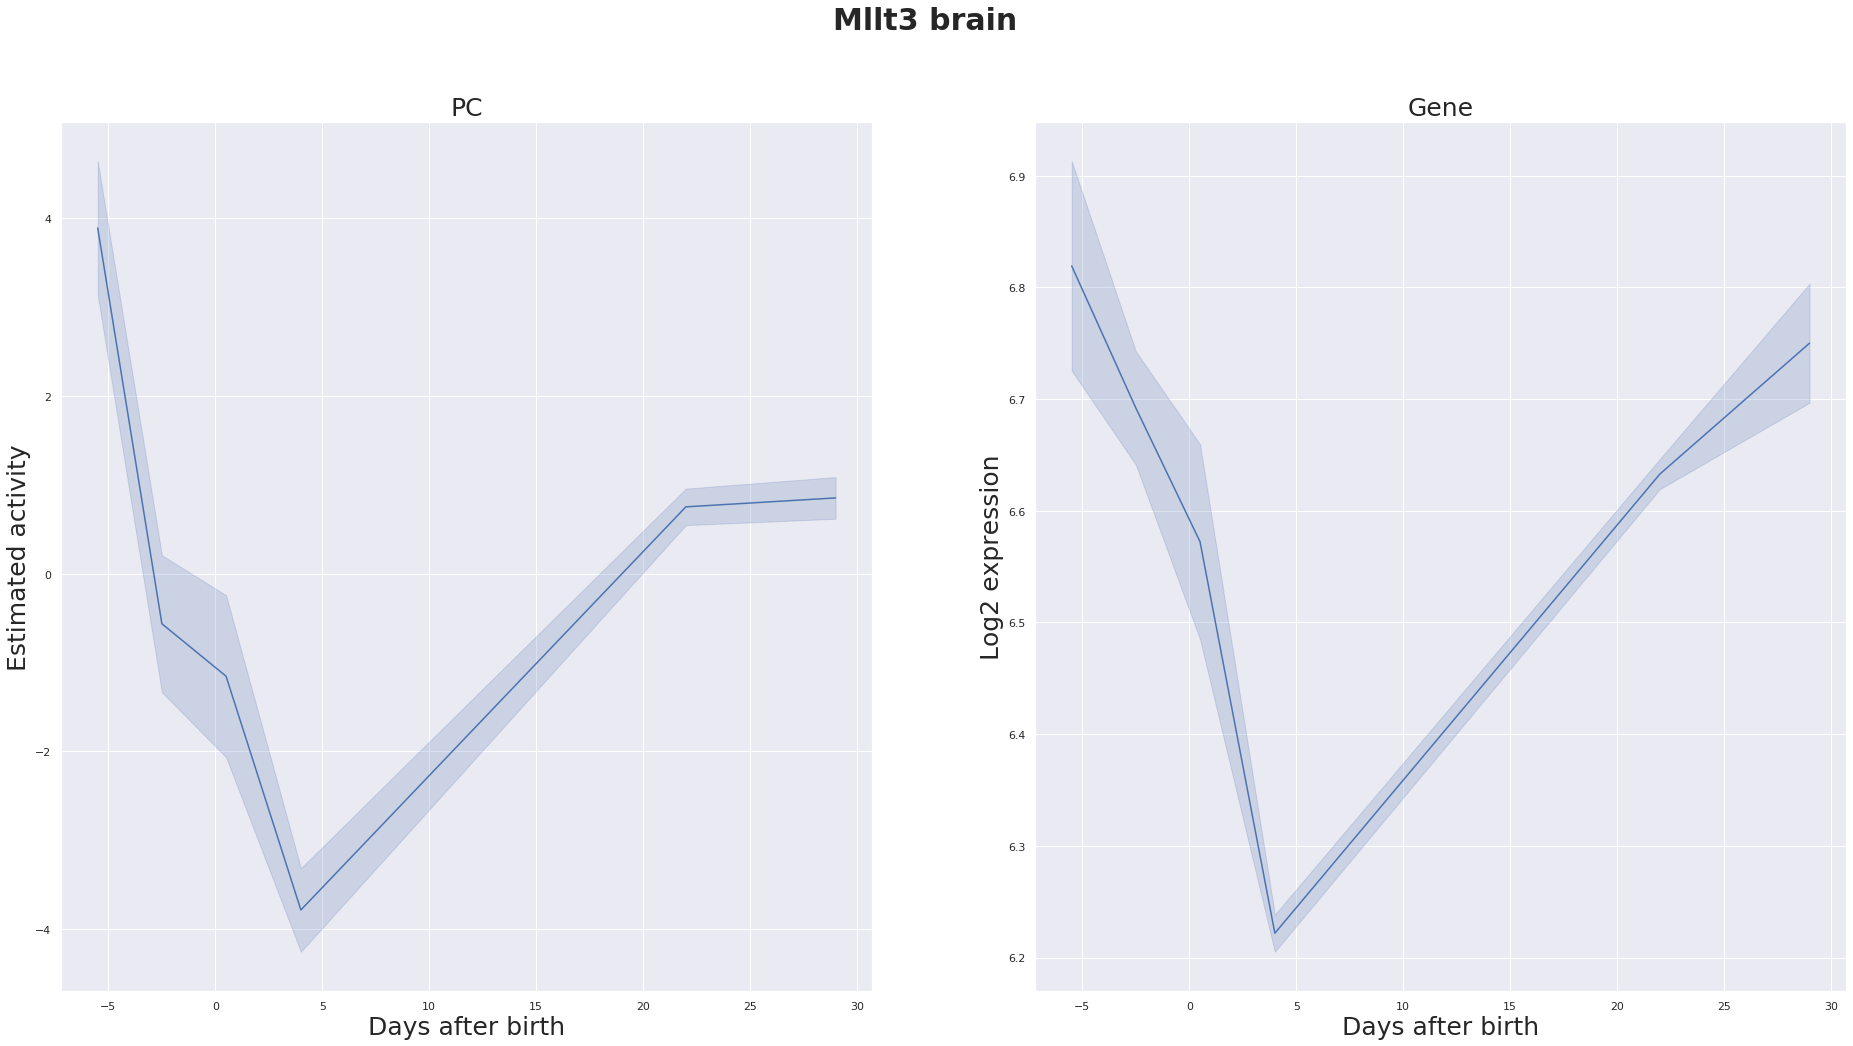
\includegraphics[width=6cm,height=3cm]{Figures&amp;Cover/Activity_Mllt3_brain_1PCremoved_filtering_False.png}
    \vspace{0.25cm}
    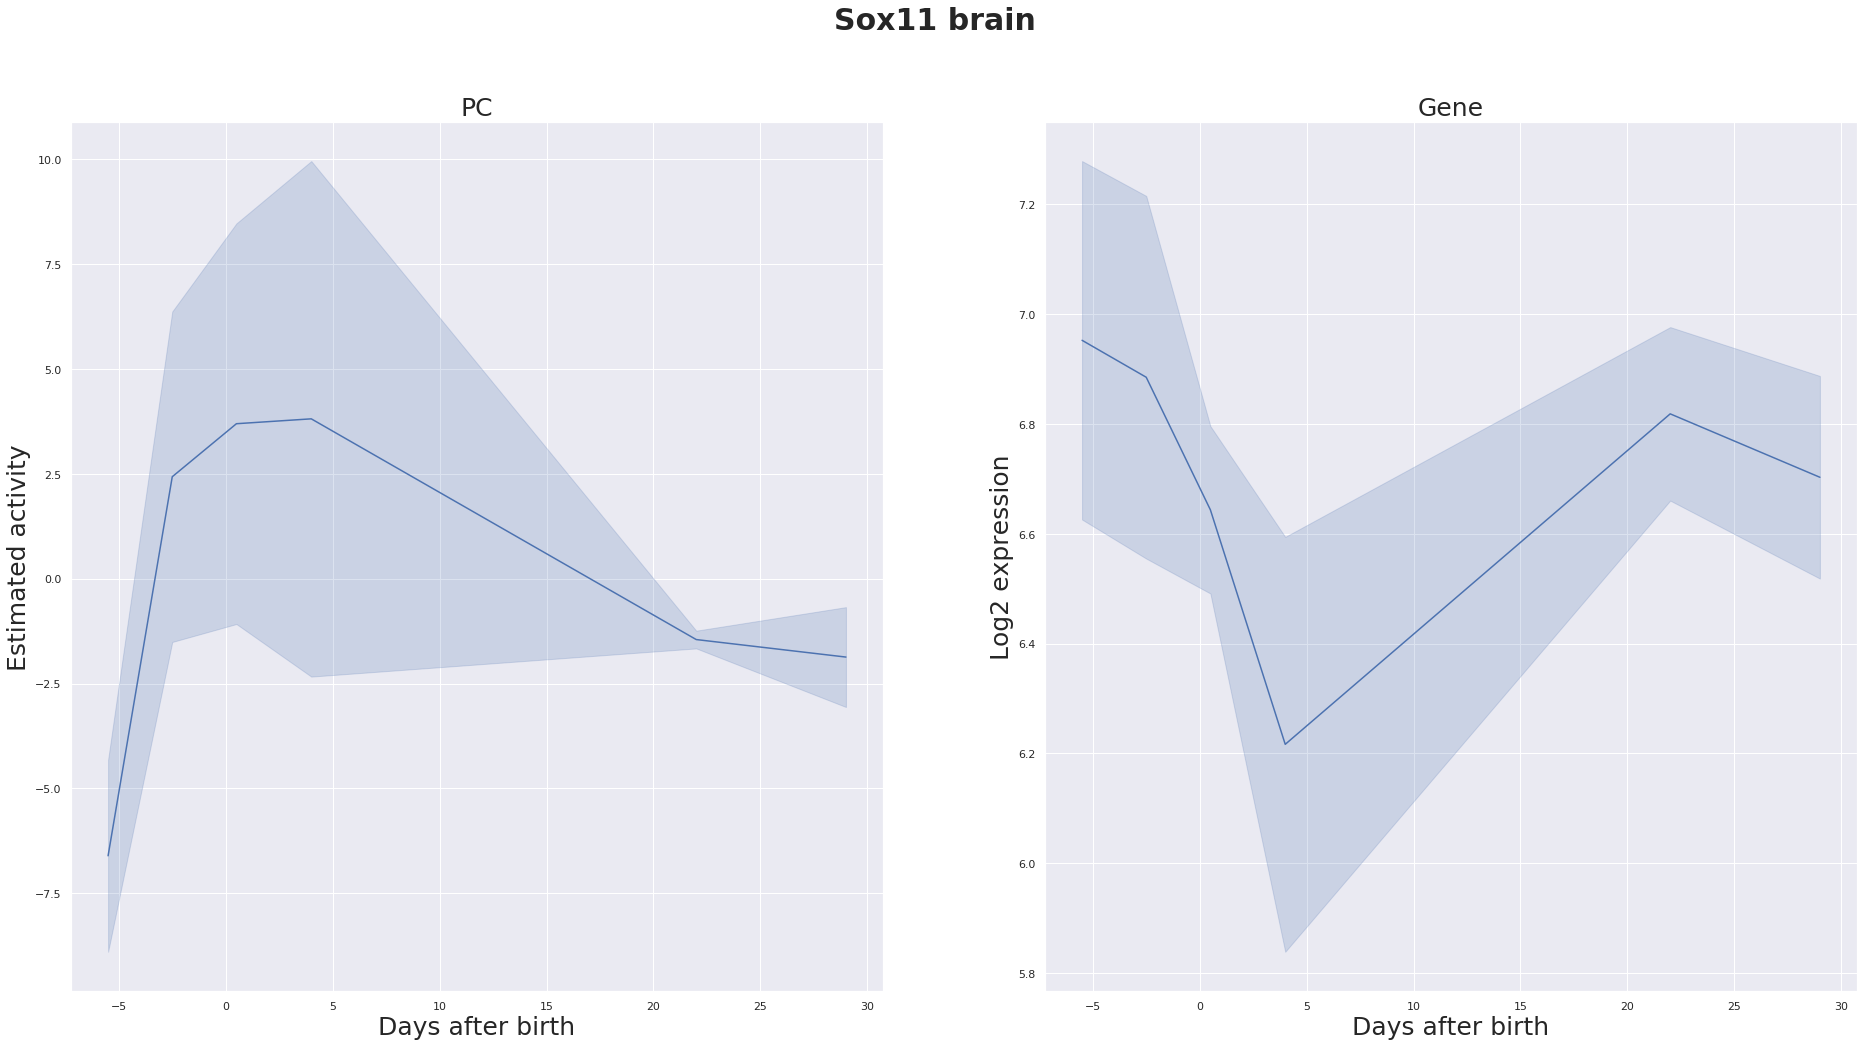
\includegraphics[width=6cm,height=3cm]{Figures&amp;Cover/Activity_Sox11_brain_1PCremoved_filtering_False.png}
    \caption{\textbf{Estimated activities of Tal1, Lmo2, Ncapg, Ikzf1, Top2a, Klf9, Brca1, Mllt3 and Sox11 in mouse brains as a functions of the mices' age, calculated using mRNA expression data from which the first \ac{PC} had been removed.} The activities were estimated by the first \ac{PC} of the mRNA expression data of the genes each \ac{TF} is likely to regulate (left figure of each pair) as well as directly through the transcription of the genes coding for each \ac{TF}, as log2-transformed \ac{RPM} transcript counts (right figure of each pair).}
    \label{fig:BrainEstsClean1}
\end{figure}    
    
\begin{figure}
    \centering
    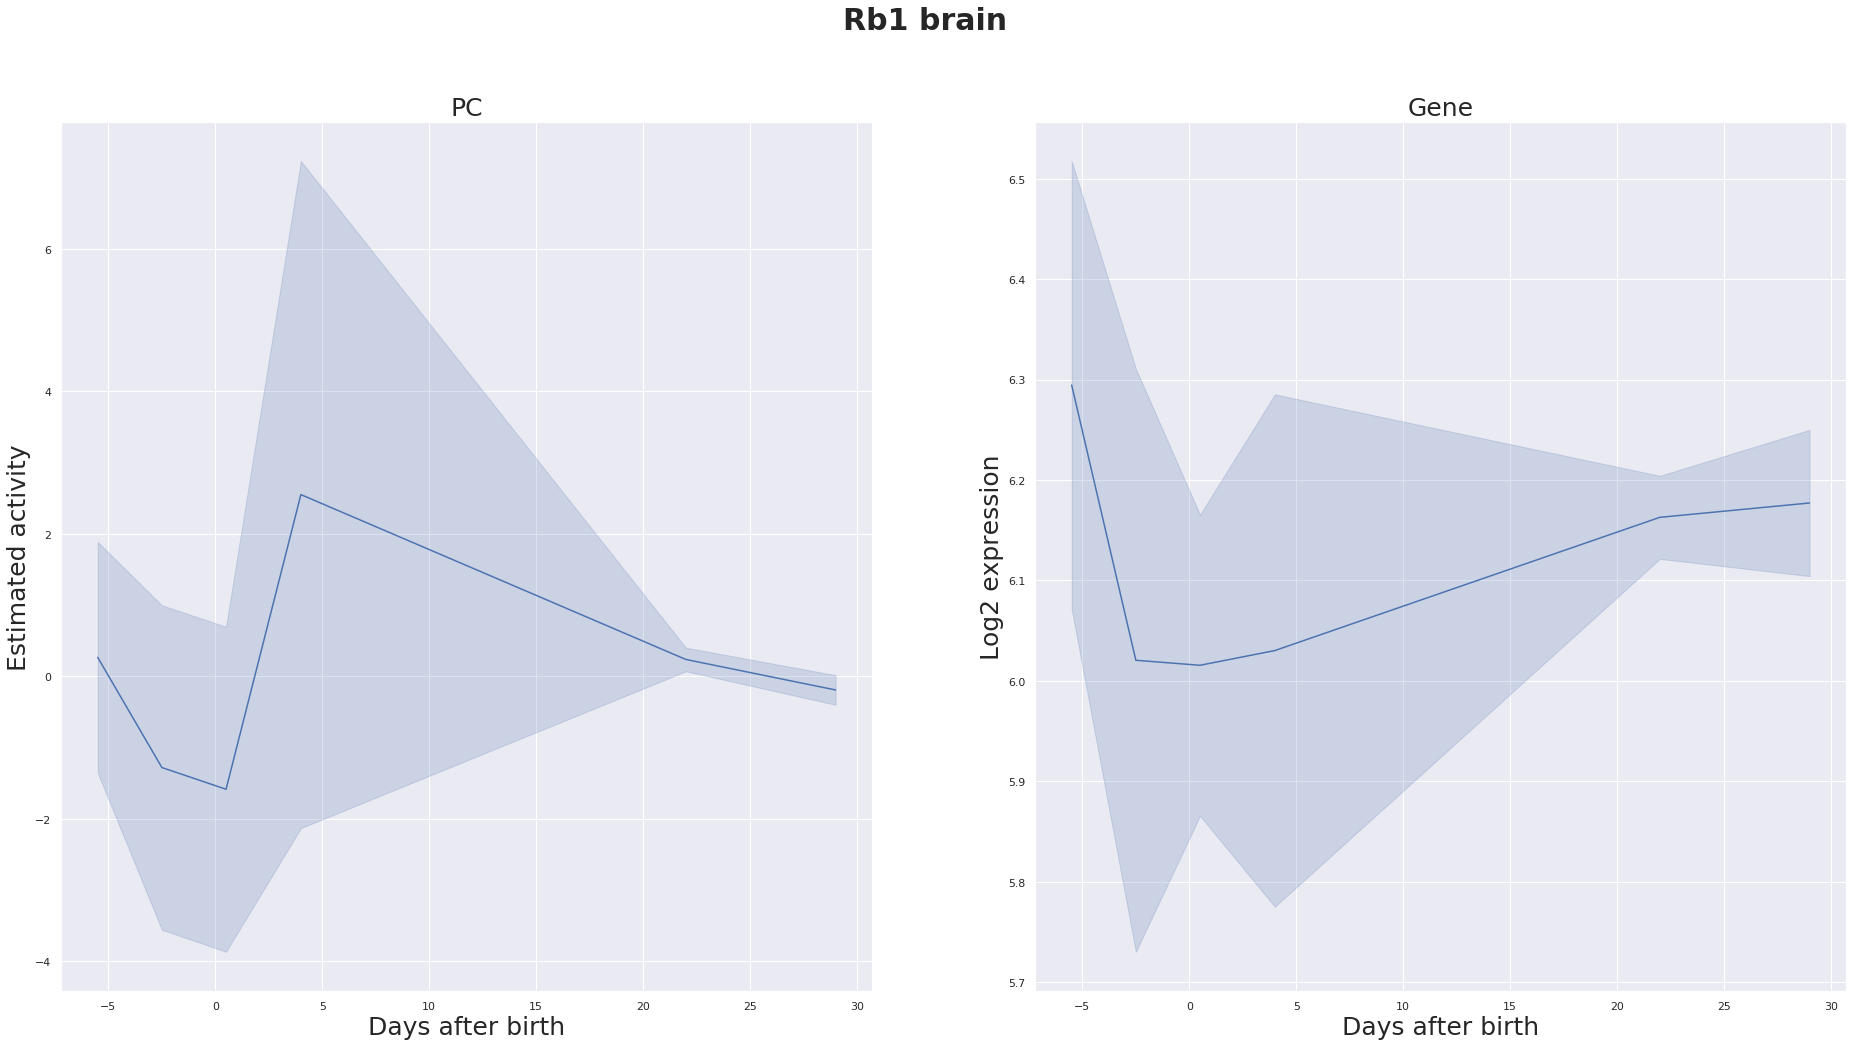
\includegraphics[width=6cm,height=3cm]{Figures&amp;Cover/Activity_Rb1_brain_1PCremoved_filtering_False.png}
    \hspace{0.25cm}
    \vspace{0.25cm}
    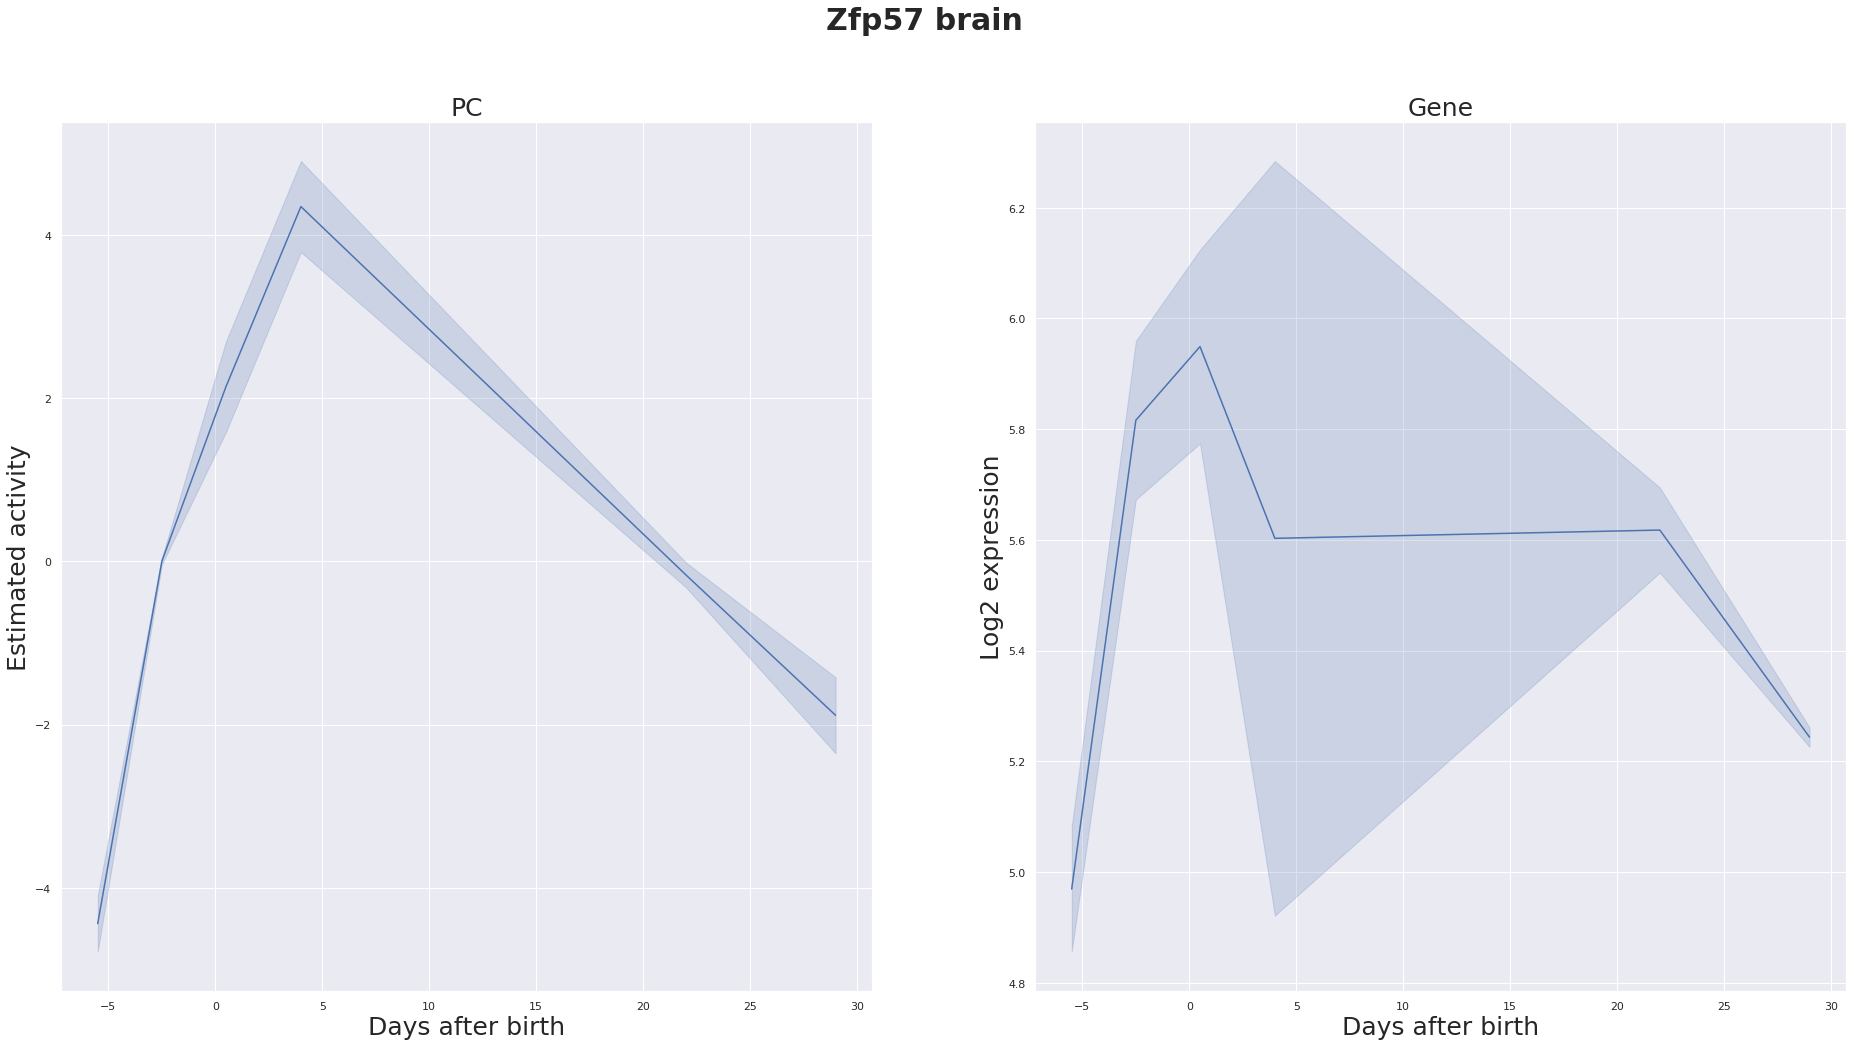
\includegraphics[width=6cm,height=3cm]{Figures&amp;Cover/Activity_Zfp57_brain_1PCremoved_filtering_False.png}
    \vspace{0.25cm}
    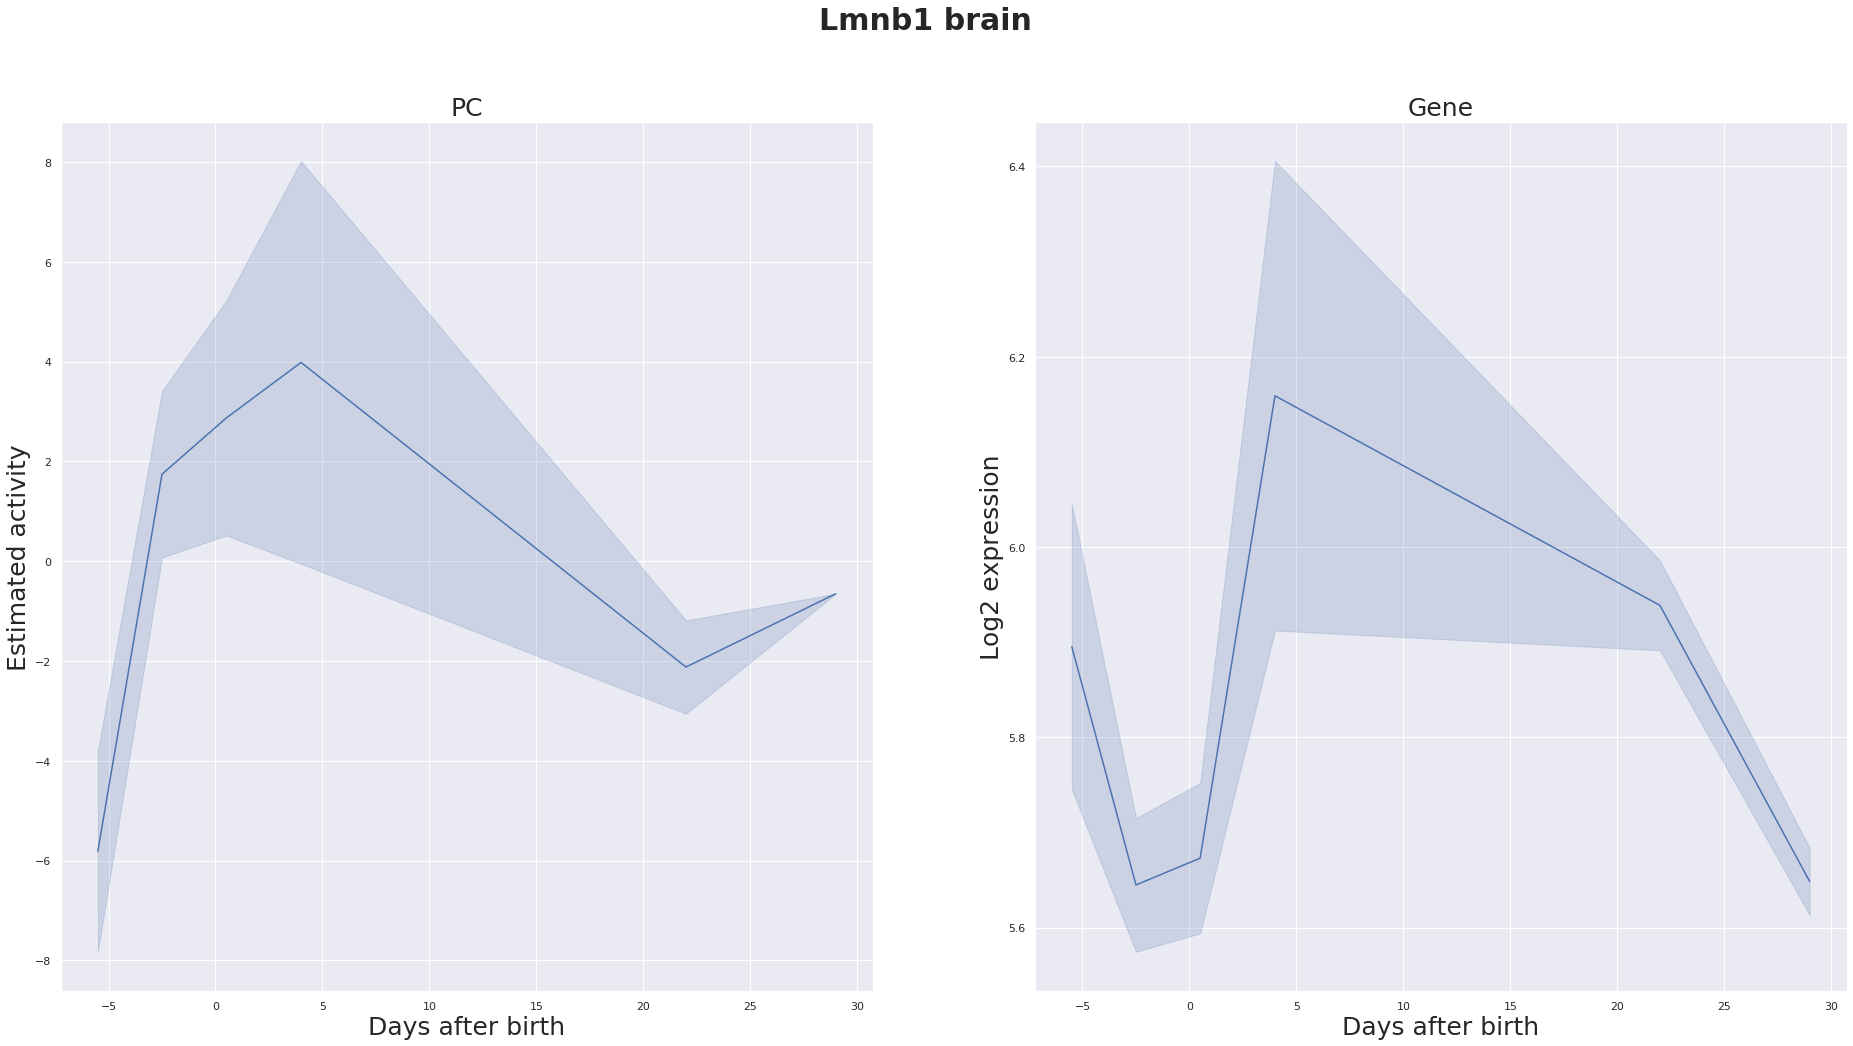
\includegraphics[width=6cm,height=3cm]{Figures&amp;Cover/Activity_Lmnb1_brain_1PCremoved_filtering_False.png}
    \hspace{0.25cm}
    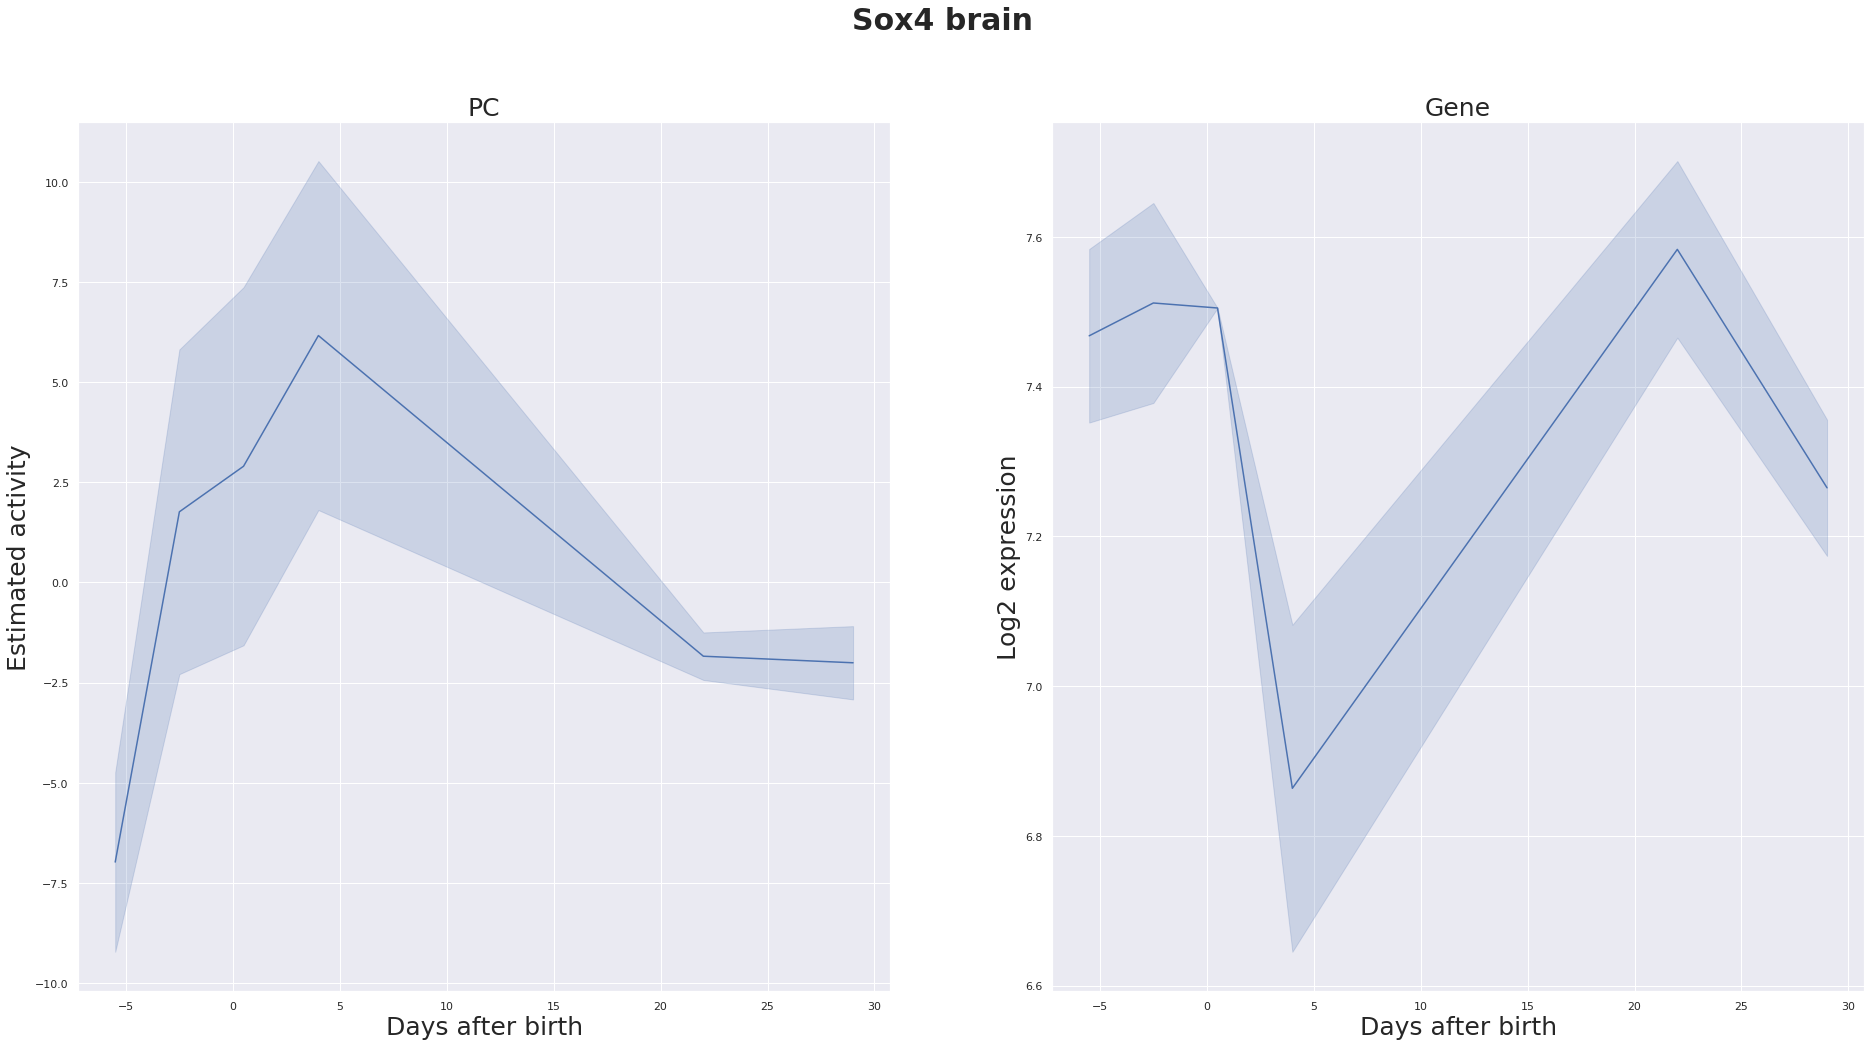
\includegraphics[width=6cm,height=3cm]{Figures&amp;Cover/Activity_Sox4_brain_1PCremoved_filtering_False.png}
    \vspace{0.25cm}
    \includegraphics[width=6cm,height=3cm]{Figures&amp;Cover/Activity_Tcf7l2_brain_1PCremoved_filtering_False.png}
    \hspace{0.25cm}
    \includegraphics[width=6cm,height=3cm]{Figures&amp;Cover/Activity_Nr1d2_brain_1PCremoved_filtering_False.png}
    \vspace{0.25cm}
    \includegraphics[width=6cm,height=3cm]{Figures&amp;Cover/Activity_Nr3c1_brain_1PCremoved_filtering_False.png}
    \hspace{0.25cm}
    \includegraphics[width=6cm,height=3cm]{Figures&amp;Cover/Activity_Satb2_brain_1PCremoved_filtering_False.png}
    \caption{\textbf{Estimated activities of Rb1, Zfp57, Lmnb1, Sox4, Tc7l2, Nr1d2, Nr3c1 and Satb2 in mouse brains as a functions of the mices' age, calculated using mRNA expression data from which the first \ac{PC} had been removed.} The activities were estimated by the first \ac{PC} of the mRNA expression data of the genes each \ac{TF} is likely to regulate (left figure of each pair) as well as directly through the transcription of the genes coding for each \ac{TF}, as log2-transformed \ac{RPM} transcript counts (right figure of each pair).}
    \label{fig:BrainEstsClean2}
\end{figure}

\begin{figure}
    \centering
    \includegraphics[width=6cm,height=3cm]{Figures&amp;Cover/Activity_Tal1_liver_1PCremoved_filtering_False.png}
    \hspace{0.25cm}
    \vspace{0.25cm}
    \includegraphics[width=6cm,height=3cm]{Figures&amp;Cover/Activity_Lmo2_liver_1PCremoved_filtering_False.png}
    \vspace{0.25cm}
    \includegraphics[width=6cm,height=3cm]{Figures&amp;Cover/Activity_Ncapg_liver_1PCremoved_filtering_False.png}
    \hspace{0.25cm}
    \includegraphics[width=6cm,height=3cm]{Figures&amp;Cover/Activity_Ikzf1_liver_1PCremoved_filtering_False.png}
    \vspace{0.25cm}
    \includegraphics[width=6cm,height=3cm]{Figures&amp;Cover/Activity_Top2a_liver_1PCremoved_filtering_False.png}
    \hspace{0.25cm}
    \includegraphics[width=6cm,height=3cm]{Figures&amp;Cover/Activity_Klf9_liver_1PCremoved_filtering_False.png}
    \vspace{0.25cm}
    \includegraphics[width=6cm,height=3cm]{Figures&amp;Cover/Activity_Brca1_liver_1PCremoved_filtering_False.png}
    \hspace{0.25cm}
    \includegraphics[width=6cm,height=3cm]{Figures&amp;Cover/Activity_Mllt3_liver_1PCremoved_filtering_False.png}
    \vspace{0.25cm}
    \includegraphics[width=6cm,height=3cm]{Figures&amp;Cover/Activity_Sox11_liver_1PCremoved_filtering_False.png}
    \caption{\textbf{Estimated activities of Tal1, Lmo2, Ncapg, Ikzf1, Top2a, Klf9, Brca1, Mllt3 and Sox11 in mouse liver as a functions of the mices' age, calculated using mRNA expression data from which the first \ac{PC} had been removed.} The activities were estimated by the first \ac{PC} of the mRNA expression data of the genes each \ac{TF} is likely to regulate (left figure of each pair) as well as directly through the transcription of the genes coding for each \ac{TF}, as log2-transformed \ac{RPM} transcript counts (right figure of each pair).}
    \label{fig:LiverEstsClean1}
\end{figure}

\begin{figure}
    \centering
    \includegraphics[width=6cm,height=3cm]{Figures&amp;Cover/Activity_Rb1_liver_1PCremoved_filtering_False.png}
    \hspace{0.25cm}
    \vspace{0.25cm}
    \includegraphics[width=6cm,height=3cm]{Figures&amp;Cover/Activity_Zfp57_liver_1PCremoved_filtering_False.png}
    \vspace{0.25cm}
    \includegraphics[width=6cm,height=3cm]{Figures&amp;Cover/Activity_Lmnb1_liver_1PCremoved_filtering_False.png}
    \hspace{0.25cm}
    \includegraphics[width=6cm,height=3cm]{Figures&amp;Cover/Activity_Sox4_liver_1PCremoved_filtering_False.png}
    \vspace{0.25cm}
    \includegraphics[width=6cm,height=3cm]{Figures&amp;Cover/Activity_Tcf7l2_liver_1PCremoved_filtering_False.png}
    \hspace{0.25cm}
    \includegraphics[width=6cm,height=3cm]{Figures&amp;Cover/Activity_Nr1d2_liver_1PCremoved_filtering_False.png}
    \vspace{0.25cm}
    \includegraphics[width=6cm,height=3cm]{Figures&amp;Cover/Activity_Nr3c1_liver_1PCremoved_filtering_False.png}
    \hspace{0.25cm}
    \includegraphics[width=6cm,height=3cm]{Figures&amp;Cover/Activity_Satb2_liver_1PCremoved_filtering_False.png}
    \caption{\textbf{Estimated activities of Rb1, Zfp57, Lmnb1, Sox4, Tc7l2, Nr1d2, Nr3c1 and Satb2 in mouse liver as a functions of the mices' age, calculated using mRNA expression data from which the first \ac{PC} had been removed.} The activities were estimated by the first \ac{PC} of the mRNA expression data of the genes each \ac{TF} is likely to regulate (left figure of each pair) as well as directly through the transcription of the genes coding for each \ac{TF}, as log2-transformed \ac{RPM} transcript counts (right figure of each pair).}
    \label{fig:LiverEstsClean2}
\end{figure}